%%%%%%%%%%%%%%%%%%%%%%%%%%%%%%%%%%%%%%%%%%%%%%%%%%%%%%%%%%%%%%%%%%%%%%%%%%%%%%%%
% Preámbulo                                                                    %
%%%%%%%%%%%%%%%%%%%%%%%%%%%%%%%%%%%%%%%%%%%%%%%%%%%%%%%%%%%%%%%%%%%%%%%%%%%%%%%%

\documentclass[11pt,a4paper,titlepage,oneside]{report}
%%% RELACIÓN DE VARIABLES A PERSONALIZAR %%%
%\def\lingua{gal}
\def\lingua{esp} % descomenta esta liña se redactarás a memoria en español
%\def\lingua{eng} % descomenta esta liña se redhttps://www.overleaf.com/project/6a0ca1f6f6d200d2d4bf51ce#actarás a memoria en inglés
\def\nome{Pablo Chantada Saborido}                             % substitúe aquí o teu nome
\def\nomedirectorA{Alejandro Rodríguez Arias}              % substitúe aquí o nome de quen dirixe
\def\nomedirectorB{Brais Cancela Barizo}             % duplica esta liña máis veces se o precisas, cambiando
                                                     % a letra final (A, B, C, D...): úsanse na portada.tex
\def\titulo{Técnicas de inteligencia artificial aplicadas en entornos simulados complejos} % substitúe aquí o título do teu TFG
%\def\titulacion{gced}                               % descomenta esta liña e comenta a seguinte se es estudante do GCED
\def\titulacion{gia}
%\def\mencion{COMPUTACIÓN}                           % descomenta a mención que che corresponda se es estudante do GEI
% \def\mencion{ENXEÑARÍA DO SOFTWARE}
%\def\mencion{ENXEÑARÍA DE COMPUTADORES}
%\def\mencion{SISTEMAS DE INFORMACIÓN}
%\def\mencion{TECNOLOXÍAS DA INFORMACIÓN}

\def\renomearcadros{si} % descomenta esta liña se redactas a memoria en español e prefires que
                         % os "cuadros" e o "índice de cuadros" se renomeen
                         % a "tablas" e "índice de tablas" respectivamente

\usepackage{estilo_tfg}
% Lista de paquetes potencialmente interesantes (uso baixo demanda)

% \usepackage{alltt}       % proporciona o entorno alltt, semellante a verbatim pero que respecta comandos
% \usepackage{enumitem}    % permite personalizar os entornos de lista
% \usepackage{eurofont}    % proporciona o comando \euro
% \usepackage{float}       % permite máis opcións para controlar obxectos flotantes (táboas, figuras)
% \usepackage{hhline}      % permite personalizar as liñas horizontais en arrays e táboas
  \usepackage{longtable}   % permite construir táboas que ocupan máis dunha páxina
% \usepackage{lscape}      % permite colocar partes do documento en orientación apaisada
% \usepackage{moreverb}    % permite personalizar o entorno verbatim
% \usepackage{multirow}    % permite crear celdas que ocupan varias filas da mesma táboa
% \usepackage{pdfpages}    % permite insertar ficheiros en PDF no documento
% \usepackage{rotating}    % permite diferentes tipos de rotacións para figuras e táboas
% \usepackage{subcaption}  % permite a inclusión de varias subfiguras nunha figura
% \usepackage{tabu}        % permite táboas flexibles
% \usepackage{tabularx}    % permite táboas con columnas de anchura determinada
\usepackage{siunitx}
\sisetup{output-decimal-marker={,}, group-separator={\,}, group-minimum-digits=4}
%%%%%%%%%%%%%%%%%%%%%%%%%%%%%%%%%%%%%%%%%%%%%%%%%%%%%%%%%%%%%%%%%%%%%%%%%%%%%%%%
% Corpo                                                                        %
%%%%%%%%%%%%%%%%%%%%%%%%%%%%%%%%%%%%%%%%%%%%%%%%%%%%%%%%%%%%%%%%%%%%%%%%%%%%%%%%

\begin{document}

 %%%%%%%%%%%%%%%%%%%%%%%%%%%%%%%%%%%%%%%%
 % Preliminares do documento            %
 %%%%%%%%%%%%%%%%%%%%%%%%%%%%%%%%%%%%%%%%

 \include{portada/portada}
 \dedicatoria{Para Ainhoa, por ser la bondad en persona.} % escribe neste comando o teu texto de dedicatoria
 \paxinaenbranco
 \begin{agradecementos}
  Agradecer a mi Madre y a Heleno, por apoyarme en todo momento y siempre darme todo lo que han podido; 
  a Ainhoa, por entenderme y apoyarme como nadie más lo hace; a Jaime, por siempre estar en vida a pesar de la distancia; a Pepe, por reavivar mi pasión y curiosidad; a mis amigos, por apoyarme durante todo el proceso; y a mis tutores Alex y Brais, por su profesionalidad, guía y enseñanzas durante todo este trabajo.
 \end{agradecementos}
 %%%%%%%%%%%%%%%%%%%%%%%%%%%%%%%%%%%%%%%%%%%%%%%%%%%%%%%%%%%%%%%%%%%%%%%%%%%%%%%%
% El abstract si lo hago mas grande se rompe
\pagestyle{empty}
\begin{abstract}
Los videojuegos en \textit{3D} ofrecen entornos experimentales excelentes para comparar distintas 
técnicas de inteligencia artificial en contextos caracterizados por una elevada complejidad perceptiva y temporal. 
En este trabajo se analizan tres enfoques: la planificación jerárquica de tareas (HTN), el aprendizaje por imitación (IL) 
y el aprendizaje por refuerzo (RL), empleando el videojuego \textit{Minecraft} como entorno de simulación. 
La objetivo común elegida consiste en localizar y talar al menos cinco troncos 
bajo restricciones de mínima omnisciencia; para ello se utiliza
una arquitectura multientorno que integra \textit{Node.js} y \textit{Python}.
Los resultados muestran que el conocimiento experto es el principal factor
diferencial: el HTN alcanza un \qty{100}{\percent} de éxito, el IL basado en
redes recurrentes un \qty{52}{\percent}, y el mejor algoritmo de RL (PPO) un
\qty{12}{\percent}. Como trabajo futuro, se propone utilizar el HTN como tutor
del agente de RL para combinar las fortalezas de ambos paradigmas.

\vspace*{25pt}

\begin{segundoresumo}
Three-dimensional video games provide an ideal testing ground for comparing artificial
intelligence techniques in scenarios with high perceptual and temporal
complexity. This work compares three paradigms: Hierarchical Task Network (HTN)
planning, imitation learning (IL), and reinforcement learning (RL), using the
video game \textit{Minecraft} as a simulation environment. The common objective consists of locating and chopping at least five logs
under limited perception constraints; to this end, a multi-environment
architecture integrating \textit{Node.js} and \textit{Python} is used.
Results show that expert knowledge is the main differentiating
factor: the HTN achieves a \qty{100}{\percent} success rate, the IL based on recurrent
networks a \qty{52}{\percent}, and the best RL algorithm a
\qty{12}{\percent}. As future work, it is proposed to use the HTN as a tutor
for the RL agent to combine the strengths of both paradigms.
\end{segundoresumo}

\vspace*{25pt}
\begin{multicols}{2}
\begin{description}
\item [\palabraschaveprincipal:] \mbox{} \\[-20pt]
    \begin{itemize}
        \item Aprendizaje por refuerzo (RL)
        \item Aprendizaje por imitación (IL)
        \item Planificación HTN
        % \item Modelos de lenguaje (LLMs)
        \item Visión por computador
        \item Agentes inteligentes
        \item Minecraft
  \end{itemize}
\end{description}
\begin{description}
\item [\palabraschavesecundaria:] \mbox{} \\[-20pt]
    \begin{itemize}
        \item Reinforcement Learning (RL)
        \item Imitation Learning (IL)
        \item HTN Planning
        % \item Large Language Models (LLMs)
        \item Computer Vision
        \item Inteligent Agents
        \item Minecraft
  \end{itemize}
\end{description}
\end{multicols}

\end{abstract}
\pagestyle{fancy}

%%%%%%%%%%%%%%%%%%%%%%%%%%%%%%%%%%%%%%%%%%%%%%%%%%%%%%%%%%%%%%%%%%%%%%%%%%%%%%%%

 \pagenumbering{roman}
 \setcounter{page}{1}
 \bstctlcite{IEEEexample:BSTcontrol}

 \tableofcontents
 \listoffigures
 \listoftables
 \clearpage
 
 \pagenumbering{arabic}
 \setcounter{page}{1}

 %%%%%%%%%%%%%%%%%%%%%%%%%%%%%%%%%%%%%%%%
 % Capítulos                            %
 %%%%%%%%%%%%%%%%%%%%%%%%%%%%%%%%%%%%%%%%

 \chapter{Introducción}
\label{chap:introduccion}

\lettrine{L}{os} entornos virtuales en \textit{3D} han resultado ser buenos escenarios para
la investigación de algoritmos de \gls{ia}.
A diferencia de entornos de juegos clásicos como el ajedrez, los entornos virtuales en \textit{3D} ofrecen
percepción visual en diferentes perspectivas (primera persona, tercera persona, etc.),
espacios de acción continuos o de alta dimensionalidad y características temporales complejas,
aumentando mucho más su dificultad y acercándolos más al funcionamiento del mundo
real~\cite{DBLP:journals/nature/SilverHMGSDSAPL16,DBLP:journals/nature/VinyalsBCMDCCPE19}.
Plataformas como Atari~\cite{DBLP:journals/nature/MnihKSRVBGRFOPB15} o VizDoom~\cite{kempka2016vizdoom}
han sido referentes clave para el uso de aprendizaje por refuerzo y planificación autónoma
en los videojuegos.

Dentro de esta familia de entornos virtuales, \textit{Minecraft} ocupa un lugar singular.
Se trata de un videojuego \textit{3D} de mundo abierto en primera persona
centrado en la recolección de recursos, la construcción de estructuras,
la fabricación de objetos y la supervivencia~\cite{guss2019minerl}. Se caracteriza por sus mundos, 
generados de forma procedimental y formados por bloques que el jugador
puede modificar, lo que genera un espacio de acciones grande y variado.
A diferencia de otros entornos de referencia, \textit{Minecraft} carece de un objetivo 
único predefinido, lo que obliga a los agentes a planificar
horizontes temporales largos con recompensas dispersas y, a menudo,
a trabajar en situaciones nunca vistas durante el entrenamiento.

El desafío más complejo que presenta el juego consiste en derrotar al \textit{Ender Dragon},
un jefe final que requiere la planificación y ejecución de una gran red de tareas anidadas entre sí.
Tarea que aún no ha sido completada usando únicamente agentes autónomos, sin ninguna intervención humana.

A nivel de progreso, todos los objetivos que plantee el jugador pueden alcanzarse de varias formas y empleando diferentes herramientas.
A partir de esta premisa, los jugadores pueden fabricar materiales y objetos específicos que requieren la recolección previa 
de una variedad de recursos, lo que da lugar a un complejo sistema de creación organizado como un árbol jerárquico
(véase el Apéndice~\ref{apx:iron-pickaxe}).

Como ejemplo, si el jugador quisiera un pico de hierro debería: recolectar primero madera rompiendo un árbol, luego fabricar una mesa de trabajo para 
fabricar nuevos objetos; dentro de ella, fabricar un pico de madera para recolectar piedra y, a continuación, un pico de piedra 
con el que extraer carbón y mineral de hierro; después, construir un horno para fundir el mineral y obtener lingotes de hierro para, 
finalmente, fabricar el pico de hierro. Además, el jugador debe encontrar en el mundo todos los recursos necesarios.

Esta tarea, que puede parecer sencilla para un jugador humano, supone un gran desafío para
los algoritmos de \gls{ia}, ya que tanto el entorno como el espacio de acciones son muy grandes y complejos,
y presentan además un fuerte componente temporal difícil de capturar.

Ante este desafío se pueden aplicar paradigmas de \gls{ia} muy diferentes entre sí,
desde la planificación simbólica basada en conocimiento experto
hasta el aprendizaje a partir de imitación o usando la propia interacción con el entorno.
Este trabajo, por tanto, compara estas tres familias: planificación jerárquica de tareas (\gls{htn}),
aprendizaje por imitación (\gls{il}) y aprendizaje por refuerzo (\gls{rl}), sobre una misma tarea
en \textit{Minecraft} y bajo idénticas condiciones de evaluación, con el fin de analizar
las fortalezas y limitaciones de cada enfoque y 
la relación entre conocimiento experto, datos y coste de cómputo.

\section{Objetivos}
El trabajo plantea las siguientes metas finales:
\begin{itemize}
    \item Diseñar e implementar agentes autónomos basados en distintos paradigmas de \gls{ia}. Específicamente \gls{htn}, \gls{il} y \gls{rl}, enfocados en la resolución de tareas en \textit{Minecraft}.
    \item Desarrollar, en caso necesario, conjuntos de datos específicos que permitan el entrenamiento de los modelos seleccionados.
    \item Definir métricas adecuadas para la evaluación del rendimiento de los agentes en el entorno.
    \item Analizar y comparar el rendimiento, eficacia y limitaciones de cada paradigma.
    \item Combinar sistemas de forma eficiente, utilizando diferentes lenguajes de programación para el desarrollo de modelos 
    y el control de agentes, así como la comunicación entre distintos entornos de desarrollo.
\end{itemize}

\section{Estructura de la Memoria}
La organización de este trabajo es la siguiente: tras el
Capítulo~\ref{chap:introduccion} de introducción, se hace una revisión del estado del arte en el
Capítulo~\ref{chap:sota}, enfocado en técnicas de \gls{ia} aplicadas a videojuegos y, 
en particular, \textit{Minecraft}. A continuación, el
Capítulo~\ref{chap:marco_teorico} introduce los fundamentos teóricos de las tres familias
de técnicas comparadas (\gls{htn}, \gls{il} y \gls{rl}), mientras que el Capítulo~\ref{chap:metodologia} detalla la metodología de
desarrollo, las fases del proyecto, su planificación y los conjuntos de datos empleados. El
Capítulo~\ref{chap:arquitectura} describe la arquitectura del sistema común a todas las
iteraciones. Sobre esta arquitectura se construyen las tres iteraciones que forman el núcleo del
trabajo: el Capítulo~\ref{chap:iter1} introduce al agente \gls{htn}, que actúa de experto;
el Capítulo~\ref{chap:iter2}, el agente \gls{il} que aprende clonando a dicho experto;
y el Capítulo~\ref{chap:iter3}, el agente \gls{rl} que aprende desde cero por interacción
con el entorno. Tras esto, en el Capítulo~\ref{chap:discusion-resultados} se comparan las tres
técnicas bajo una métrica común y se analiza la relación entre conocimiento experto, datos
y coste de cómputo. Por último, se dedica el Capítulo~\ref{chap:conclusions}
a exponer las conclusiones y las posibles líneas futuras de investigación
obtenidas del análisis realizado en el trabajo.
 \chapter{Estado del Arte}
\label{chap:sota}

\lettrine{E}{n} este capítulo se ofrece una explicación del estado del arte sobre 
el uso de videojuegos como entorno de investigación en \gls{ia}, enfocándose especialmente en \textit{Minecraft}. 
Se describen los trabajos más relevantes en el ámbito de los videojuegos, haciendo especial énfasis
en aquellos que utilizan \textit{Minecraft} como entorno de experimentación.

Los juegos han sido un buen campo de prueba para el desarrollo de la \gls{ia}, 
gracias a su capacidad para simular entornos complejos e interactivos, y a la posibilidad de medir el 
rendimiento de los agentes de manera objetiva. 
Desde juegos clásicos con espacios de acción limitados, como el ajedrez~\cite{DBLP:journals/corr/abs-1712-01815}
o el \textit{Go}~\cite{DBLP:journals/nature/SilverHMGSDSAPL16}, que pese a disponer de un espacio de acciones reducido 
generan un espacio de estados prácticamente infinito, hasta juegos de estrategia en tiempo real con espacios de acciones enormes, 
como \textit{StarCraft}~\cite{DBLP:journals/nature/VinyalsBCMDCCPE19} o \textit{Dota 2}~\cite{DBLP:journals/corr/abs-1912-06680},
con un número de estados casi imposible de explorar.

La temática común entre estos artículos es el uso del \gls{rl} (clásico o profundo) para entrenar agentes
que puedan competir a nivel humano o superarlo. A diferencia de los juegos de mesa mencionados anteriormente, que
se basan en turnos, ejemplos como \textit{Space Invaders}
o \textit{Pong} requieren una percepción visual y una respuesta rápida para interactuar con el entorno de forma óptima, 
lo que los convierte en un campo de prueba excelente para el \gls{drl},
con las \gls{dqn}~\cite{DBLP:journals/nature/MnihKSRVBGRFOPB15} como una de las primeras aproximaciones significativas en mezclar
refuerzo clásico con aprendizaje profundo.

\section{Técnicas de IA en Videojuegos}
Entre los enfoques aplicados a videojuegos, el \gls{drl} ha producido resultados destacables. 
Las redes \gls{dqn} alcanzaron un rendimiento comparable al
de jugadores humanos profesionales en un conjunto de \num{49} juegos de \textit{Atari}~\cite{DBLP:journals/nature/MnihKSRVBGRFOPB15},
\textit{AlphaStar} llegó a nivel Gran Maestro en \textit{StarCraft~II}~\cite{DBLP:journals/nature/VinyalsBCMDCCPE19}
y \textit{OpenAI Five} superó a equipos profesionales en \textit{Dota~2}~\cite{DBLP:journals/corr/abs-1912-06680}.
Su principal limitación es la necesidad de una gran cantidad de interacciones con el
entorno y el diseño de una función de recompensa correcta.

Por otra parte, las \gls{htn} han demostrado ser competitivas
en juegos de estrategia en tiempo real como \textit{StarCraft}~\cite{DBLP:conf/ijcai/OntanonB15},
produciendo comportamientos deterministas e interpretables sin necesidad de
entrenamiento, aunque a costa de requerir conocimiento del dominio codificado
manualmente.

Sin embargo, con la llegada de los \gls{transformer}~\cite{DBLP:conf/nips/VaswaniSPUJGKP17}, 
se han empezado a aplicar estas técnicas a la investigación en videojuegos con resultados 
prometedores~\cite{DBLP:conf/nips/BakerAZHTEHSC22, DBLP:journals/corr/abs-2305-16291, DBLP:conf/nips/FanWJMYZTHZA22, oasis2024}. 
Estas aproximaciones difieren entre sí: algunas emplean un \gls{llm} para generar directamente las acciones o el código que controla al agente 
en lugar de una red neuronal entrenada por refuerzo. 
En el caso de \textit{Voyager}~\cite{DBLP:journals/corr/abs-2305-16291}, el \gls{llm} genera código \textit{JavaScript}
para controlar a un agente en \textit{Minecraft} en función de su entorno. Otras, como \textit{Oasis}~\cite{oasis2024},
emplean el \gls{transformer} como modelo generativo para construir un clon interactivo de \textit{Minecraft}.

\section{Minecraft como Entorno de Investigación}
Actualmente existen diversos trabajos relacionados con el uso de \textit{Minecraft} como
entorno de investigación en \gls{ia},
como el proyecto \textit{MineRL}~\cite{guss2019minerl}, que proporciona un conjunto de datos y un
entorno de simulación para entrenar agentes \gls{rl} en \textit{Minecraft}.

En esta misma línea, \textit{MineDojo}~\cite{DBLP:conf/nips/FanWJMYZTHZA22} amplía el enfoque con un
conjunto masivo de tareas abiertas y una extensa base de conocimiento multimodal extraída de Internet (vídeos, \textit{wiki} y foros).

En el ámbito de los \gls{llm}, \textit{Mindcraft}~\cite{mindcraft2025} es un \gls{mas} basado en \gls{llm} para el razonamiento colaborativo,
en el que los agentes generan código \textit{JavaScript} para actuar en \textit{Minecraft}, de forma similar al enfoque empleado por
\textit{Voyager}~\cite{DBLP:journals/corr/abs-2305-16291}, cuya arquitectura se muestra en la Figura~\ref{fig:Voyager} (página~\pageref{fig:Voyager}).
El objetivo a largo plazo de estos sistemas es completar el juego de forma totalmente autónoma, sin intervención humana.

\begin{figure}[htbp]
  \centering
  \resizebox{\textwidth}{!}{
  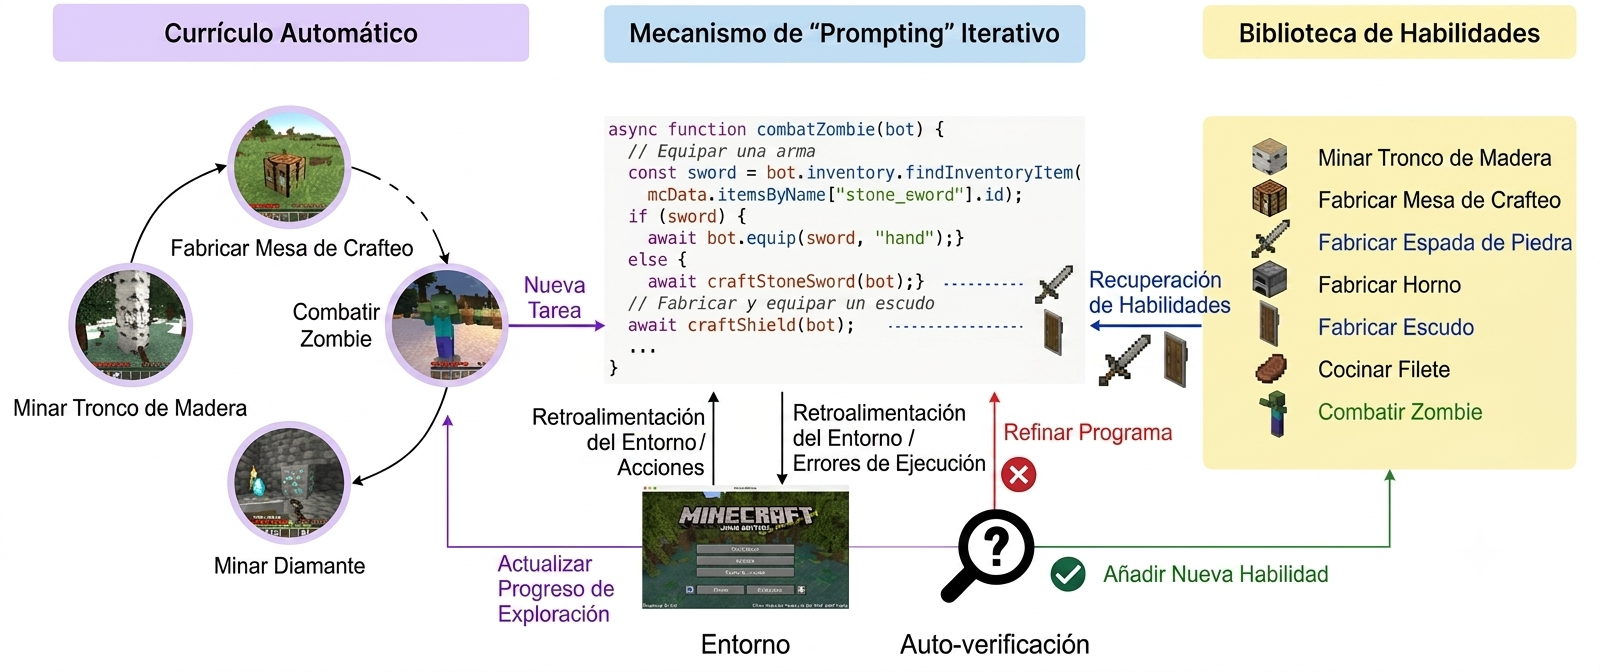
\includegraphics[width=1\textwidth]{imaxes/02_sota/voyager.png}
  }
  \caption[Arquitectura del agente Voyager]{Arquitectura de \textit{Voyager}~\cite{DBLP:journals/corr/abs-2305-16291},
  un sistema basado en \gls{llm} para controlar un agente en \textit{Minecraft}. El \gls{llm} genera código \textit{JavaScript} para controlar
  al agente en función de su entorno y construye de forma incremental una biblioteca de habilidades reutilizables.}
  \label{fig:Voyager}
\end{figure}

\section{Técnicas de IA aplicadas a Minecraft}
\subsection{Aprendizaje por Imitación}
El referente de \gls{il} en \textit{Minecraft} es \gls{vpt}~\cite{DBLP:conf/nips/BakerAZHTEHSC22},
que preentrena una \gls{política} sobre \num{70000} horas de vídeo sin etiquetar,
logrando comportamientos complejos por imitación. Su limitación
principal es el desajuste entre los estados del experto y los que explora el
aprendiz (\gls{distribution-shift}). Para mitigarlo, \gls{dagger}~\cite{DBLP:journals/jmlr/RossGB11} 
emplea al experto sobre los estados recorridos para corregir los errores cometidos por el aprendiz,
aunque el artículo original no se implementó en \textit{Minecraft}.

\subsection{Aprendizaje por Refuerzo}
En \textit{Minecraft}, la complejidad y ambigüedad de las recompensas, junto con los largos horizontes temporales, 
incrementan tanto el coste como la dificultad del entrenamiento. Dentro de estas aproximaciones, los enfoques que
alcanzan un buen rendimiento dependen de recursos difíciles de replicar en \textit{hardware} común: 
\gls{vpt}~\cite{DBLP:conf/nips/BakerAZHTEHSC22} se apoya en un preentrenamiento masivo sobre decenas de 
miles de horas de vídeo, y un \gls{world-model}
como \textit{DreamerV3}~\cite{DBLP:journals/corr/abs-2301-04104} requiere entrenamientos muy prolongados
para resolver tareas de horizonte largo. Como respuesta a este coste, la competición \textit{MineRL}~\cite{guss2019minerl} surgió
para incentivar la eficiencia muestral, y trabajos como el de
Scheller et al.~\cite{DBLP:journals/corr/abs-2003-06066}
mostraron que incorporar demostraciones humanas reduce el número de
interacciones necesarias, aunque sin eliminar por completo la
dependencia de cómputo.
 \chapter{Marco Teórico}
\label{chap:marco_teorico}

\lettrine{E}{n} este capítulo se presenta una breve explicación de las técnicas implementadas en este trabajo.
Se describen los conceptos de planificación simbólica (\gls{htn}), aprendizaje por imitación (\gls{il}) y aprendizaje por refuerzo (\gls{rl}),
así como las familias de algoritmos en las que se basan.

\section{Planificación Simbólica}
La planificación simbólica se caracteriza por ser un enfoque interpretable debido a su funcionamiento basado en reglas,
las cuales definen los estados, acciones y objetivos sobre los que opera el agente, determinando el mundo sobre el que actúa y el plan que debe seguir para cumplir su objetivo.
Dentro de la planificación simbólica existen diferentes paradigmas:

\begin{itemize}
    \item \gls{strips}~\cite{DBLP:journals/ai/FikesN71}: utiliza un \gls{solver} que, dado un mundo (estado), 
    un conjunto de operadores aplicables (acciones) que transforman el mundo y un objetivo a alcanzar, 
    encuentra una secuencia de acciones que transforma el estado inicial en uno que cumple el objetivo.

    \item \gls{sat}~\cite{DBLP:conf/ecai/KautzS92}: utiliza técnicas de satisfacibilidad para encontrar planes que 
    cumplan con las restricciones del dominio. Al igual que \gls{strips}, utiliza un \gls{solver}.

    \item \gls{htn}~\cite{DBLP:conf/aips/ErolHN94, DBLP:conf/ijcai/OntanonB15}: con una base similar a \gls{strips}, 
    pero de forma más jerárquica. En lugar de buscar la secuencia de acciones únicamente a partir del objetivo, 
    las tareas se descomponen recursivamente en subtareas y acciones, formando un árbol de descomposición.
\end{itemize}

El paradigma seleccionado para este trabajo es el de las \gls{htn}, por su capacidad para modelar comportamientos 
complejos de forma jerárquica, similar a la forma en la que se progresa en \textit{Minecraft}.
En lugar de partir únicamente de un objetivo y dejar que el \gls{solver} busque la secuencia de acciones, 
una \gls{htn} descompone el objetivo en tareas, para las cuales el programador indica cómo se resuelven o cómo 
se dividen en subtareas más sencillas.
La planificación se convierte entonces, en el recorrido de un árbol de tareas y subtareas.
El comportamiento del agente se basa en tareas, que pueden ser de tres tipos:

\begin{itemize}
    \item \textbf{Primitiva}: se resuelve ejecutando una única acción directa sobre el mundo, 
    siempre que se cumplan sus precondiciones.

    \item \textbf{Compuesta}: no se ejecuta directamente, sino que se descompone mediante uno o varios \textbf{métodos}. 
    Cada método es una forma de resolver la tarea usando una secuencia de subtareas (primitivas u otras compuestas). 
    El uso de varios métodos para la misma tarea permite al \gls{planificador} elegir, según el estado, cómo resolverla.

    \item \textbf{Objetivo}: describe un estado deseado del mundo que el \gls{planificador} debe alcanzar, seleccionando, 
    descomponiendo y ejecutando las tareas (compuestas y primitivas) disponibles.
\end{itemize}

Como ejemplo, consideremos la tarea de obtener un pico de piedra en \textit{Minecraft}.
Se trata de una tarea compuesta que se descompone en una cadena de subtareas: \emph{conseguir madera}, 
\emph{fabricar un pico de madera}, \emph{minar piedra} y \emph{fabricar el pico de piedra}.
Cada una de ellas es a su vez compuesta y se sigue descomponiendo hasta llegar a primitivas como \emph{minar un bloque} o 
\emph{fabricar un objeto} en la mesa de trabajo.
El estado de tener un pico de piedra en el inventario actúa como indicativo de éxito.

Una de las principales ventajas de las \gls{htn} es su capacidad de replanificación.
Si una tarea falla durante la ejecución, el \gls{planificador} puede identificar la causa y reaccionar, 
ya sea modificando el mundo o aplicando un método alternativo para la tarea.
En el ejemplo anterior, si el agente intenta minar piedra pero no encuentra ningún bloque accesible, 
puede explorar el entorno para acercarse a una zona con piedra; y si descubre que ha roto el pico de madera, 
puede rehacer la subtarea de fabricarlo antes de continuar.

\section{Aprendizaje por Imitación}
\label{sec:marco-il}
El aprendizaje por imitación (\gls{il}) busca obtener una \gls{política} a partir de un conjunto de demostraciones de un experto.
Una \gls{política} $\pi_\theta$, parametrizada por $\theta$, puede ser \emph{estocástica}, asignando a 
cada estado $s \in \mathcal{S}$ una distribución de probabilidad sobre las acciones ($\mathcal{A})$:
\begin{equation}
    \pi_\theta : \mathcal{S} \rightarrow \Delta(\mathcal{A})
\end{equation}

En esta expresión, la \gls{política} devuelve la probabilidad de tomar la acción $a$ en el estado $s$ (p.\,ej.\ \gls{sac}).

También puede ser \emph{determinista}, cuando devuelve una única acción $a = \pi_\theta(s)$ (p.\,ej.\ \gls{dqn}), quedando:
\begin{equation}
    \pi_\theta : \mathcal{S} \rightarrow \mathcal{A}
\end{equation}

La ventaja de la imitación frente al refuerzo es la eliminación de la función de recompensa, que es el mecanismo que 
guía el \gls{rl}, lo que permite al agente aprender comportamientos en entornos complejos 
sin necesidad de diseñar recompensas manualmente~\cite{DBLP:journals/tcyb/ZareKKN24}.
Dentro del \gls{il} existen múltiples técnicas; en este trabajo se mencionan dos por su buen encaje al problema planteado:

\begin{itemize}
    \item \textbf{Clonado de comportamiento} (\gls{bc}): planteado como un problema de \gls{aprendizaje-supervisado}.
    Dado un conjunto de pares \textit{OBSERVACIÓN-ACCIÓN} generados por el experto, se entrena un modelo que predice 
    la acción que el experto habría tomado. La principal limitación del \gls{bc} es el \gls{distribution-shift}~\cite{DBLP:journals/jmlr/RossGB11}.

    \item \textbf{Métodos interactivos} (\gls{dagger}~\cite{DBLP:journals/jmlr/RossGB11}): el experto ayuda durante 
    el aprendizaje. El aprendiz ejecuta la \gls{política} aprendida, el experto etiqueta los estados visitados y estos se 
    incorporan al conjunto de entrenamiento. Esto reduce el \gls{distribution-shift} de las técnicas \gls{offline}.
\end{itemize}

\section{Aprendizaje por Refuerzo}
\label{sec:marco-rl}
El aprendizaje por refuerzo (\gls{rl}) busca aprender una \gls{política} propia mediante interacción con el entorno.
El agente realiza acciones, observa el resultado y recibe una recompensa que indica la calidad de su comportamiento, 
como se ilustra en la Figura~\ref{fig:rl-basics} (página~\pageref{fig:rl-basics}).

\begin{figure}[htbp]
    \centering
    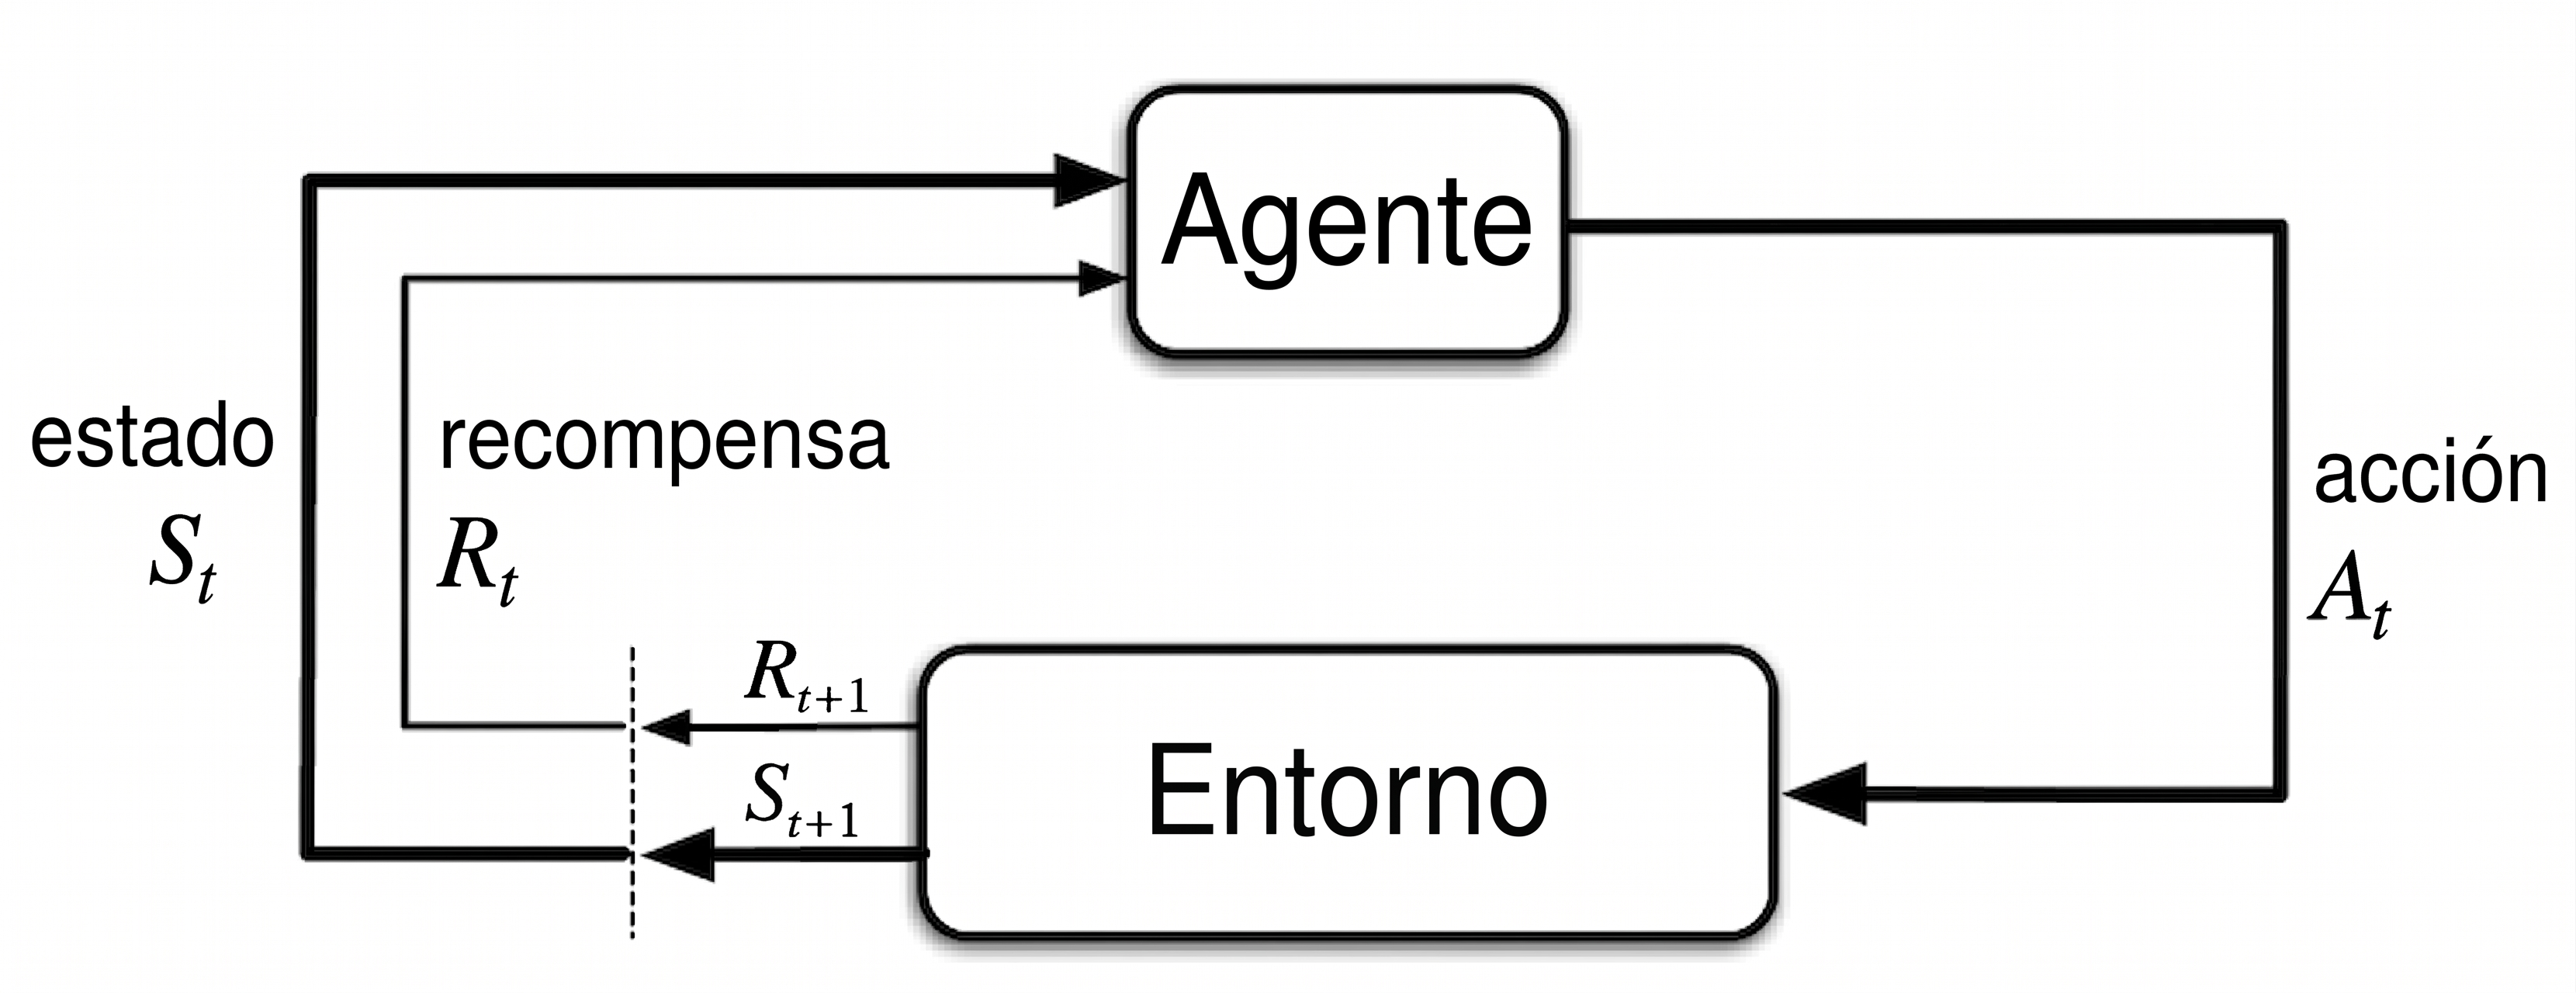
\includegraphics[width=0.6\textwidth]{imaxes/03_marco/rl_basics.png}
    \caption[Ilustración del proceso básico de aprendizaje por refuerzo]{Proceso iterativo del aprendizaje por refuerzo.
    El agente observa el estado del entorno, ejecuta una acción según su \gls{política} y recibe una recompensa y un nuevo estado. 
    Adaptada de \textit{Reinforcement Learning: An Introduction}~\cite{DBLP:books/lib/SuttonB2018}.}
    \label{fig:rl-basics}
\end{figure}

El problema se plantea habitualmente como un \gls{mdp}~\cite{DBLP:books/wi/Puterman94}, que formaliza la interacción 
asumiendo que el siguiente estado y la recompensa dependen únicamente del estado actual y la acción tomada:
\begin{equation}
    P(X_{n+1} = j \mid X_n = i, A_n = a)
\end{equation}
donde $X_n$ es el estado en el instante $n$ (con valor $i$), $A_n$ la acción tomada en ese
instante ($a$) y $X_{n+1}$ el estado resultante (con valor $j$); es decir, la probabilidad
de transitar al estado $j$ depende únicamente del estado y la acción actuales.
    
El objetivo del agente, por tanto, es maximizar el \textit{retorno esperado}, definido como la suma
descontada de las recompensas obtenidas a lo largo de la interacción:
\begin{equation}
    J(\pi) = \mathbb{E}_{\pi}\!\left[\sum_{t=0}^{\infty} \gamma^{t}\, r_t\right]
\end{equation}
donde $r_t$ es la recompensa recibida en el paso $t$, $\gamma \in [0,1)$ es el
\textit{factor de descuento} (que resta peso a las recompensas más lejanas) y
$\mathbb{E}_{\pi}[\cdot]$ denota el valor esperado siguiendo la \gls{política} $\pi$.

Para evaluar la calidad de las decisiones se define la \textit{función de valor-acción}
$Q^{\pi}(s,a)$, que estima el retorno esperado al ejecutar la acción $a$ en el estado $s$
y seguir después la \gls{política} $\pi$:
\begin{equation}
    Q^{\pi}(s,a) = \mathbb{E}_{\pi}\!\left[\sum_{t=0}^{\infty} \gamma^{t}\, r_t
    \;\middle|\; s_0 = s,\; a_0 = a\right]
\end{equation}

Esta función satisface la \textit{ecuación de Bellman}, que divide un problema complejo en subproblemas más simples, expresando el valor de una decisión actual en función de la recompensa inmediata y del valor de los estados futuros. Con ello, se puede expresar de forma recursiva
en términos del estado y la acción siguientes ($s'$ y $a'$):
\begin{equation}
    Q^{\pi}(s,a) = \mathbb{E}\!\left[\, r + \gamma\, \mathbb{E}_{a'\sim\pi}\big[Q^{\pi}(s',a')\big]\,\right]
\end{equation}

Aunque la ecuación de Bellman propaga teóricamente el valor hacia las decisiones anteriores,
en tareas de largo horizonte con recompensas escasas esta propagación se vuelve lenta y la señal
de aprendizaje se debilita: el agente apenas recibe recompensa hasta completar una secuencia larga
de acciones, lo que dificulta en la práctica atribuir correctamente el valor a cada decisión.
Para mitigar esto se utilizan recompensas intermedias (\gls{reward-shaping}) que guían la exploración.

Por ejemplo, en la tarea de \gls{woodcutting}, si solo se premiara talar árboles, el agente no aprendería cómo orientarse, 
moverse o interactuar con el entorno. Por ello se añaden recompensas intermedias por aproximarse al árbol, apuntar o golpearlo.

En este trabajo se analizan tres familias de \gls{drl}, diferenciadas de los enfoques clásicos por el uso de 
\gls{aprendizaje-automatico} para aprender la \gls{política}:

\begin{itemize}
    \item \textbf{Basados en valor}: aprenden una función $Q(s,a)$ y seleccionan la acción de mayor valor. 
    El ejemplo más representativo son las \gls{dqn}~\cite{DBLP:journals/nature/MnihKSRVBGRFOPB15}, 
    que usan redes neuronales y un \gls{replay-buffer}.

    \item \textbf{Gradiente de \gls{política}}: optimizan directamente la \gls{política} mediante ascenso de gradiente. 
    El referente es \gls{ppo}~\cite{DBLP:journals/corr/SchulmanWDRK17}.

    \item \textbf{Actor-crítico}: combinan ambos enfoques, con un actor que produce la \gls{política} y 
    un crítico que evalúa su calidad. El referente es \gls{sac}~\cite{DBLP:journals/corr/abs-1801-01290}.
\end{itemize}

Se añade una taxonomía adicional~\cite{DBLP:books/lib/SuttonB2018}, ilustrada en la Figura~\ref{fig:on-vs-off} (página~\pageref{fig:on-vs-off}):

\begin{itemize}
    \item \textbf{\Gls{on-policy}}: el agente aprende de la \gls{política} que ejecuta.
    \item \textbf{\Gls{off-policy}}: el agente aprende de experiencias generadas por \glspl{política} anteriores mediante un \gls{replay-buffer}.
\end{itemize}

% No les pongo aqui el resize pa que entren bien
\begin{figure}[htbp]
    \centering
    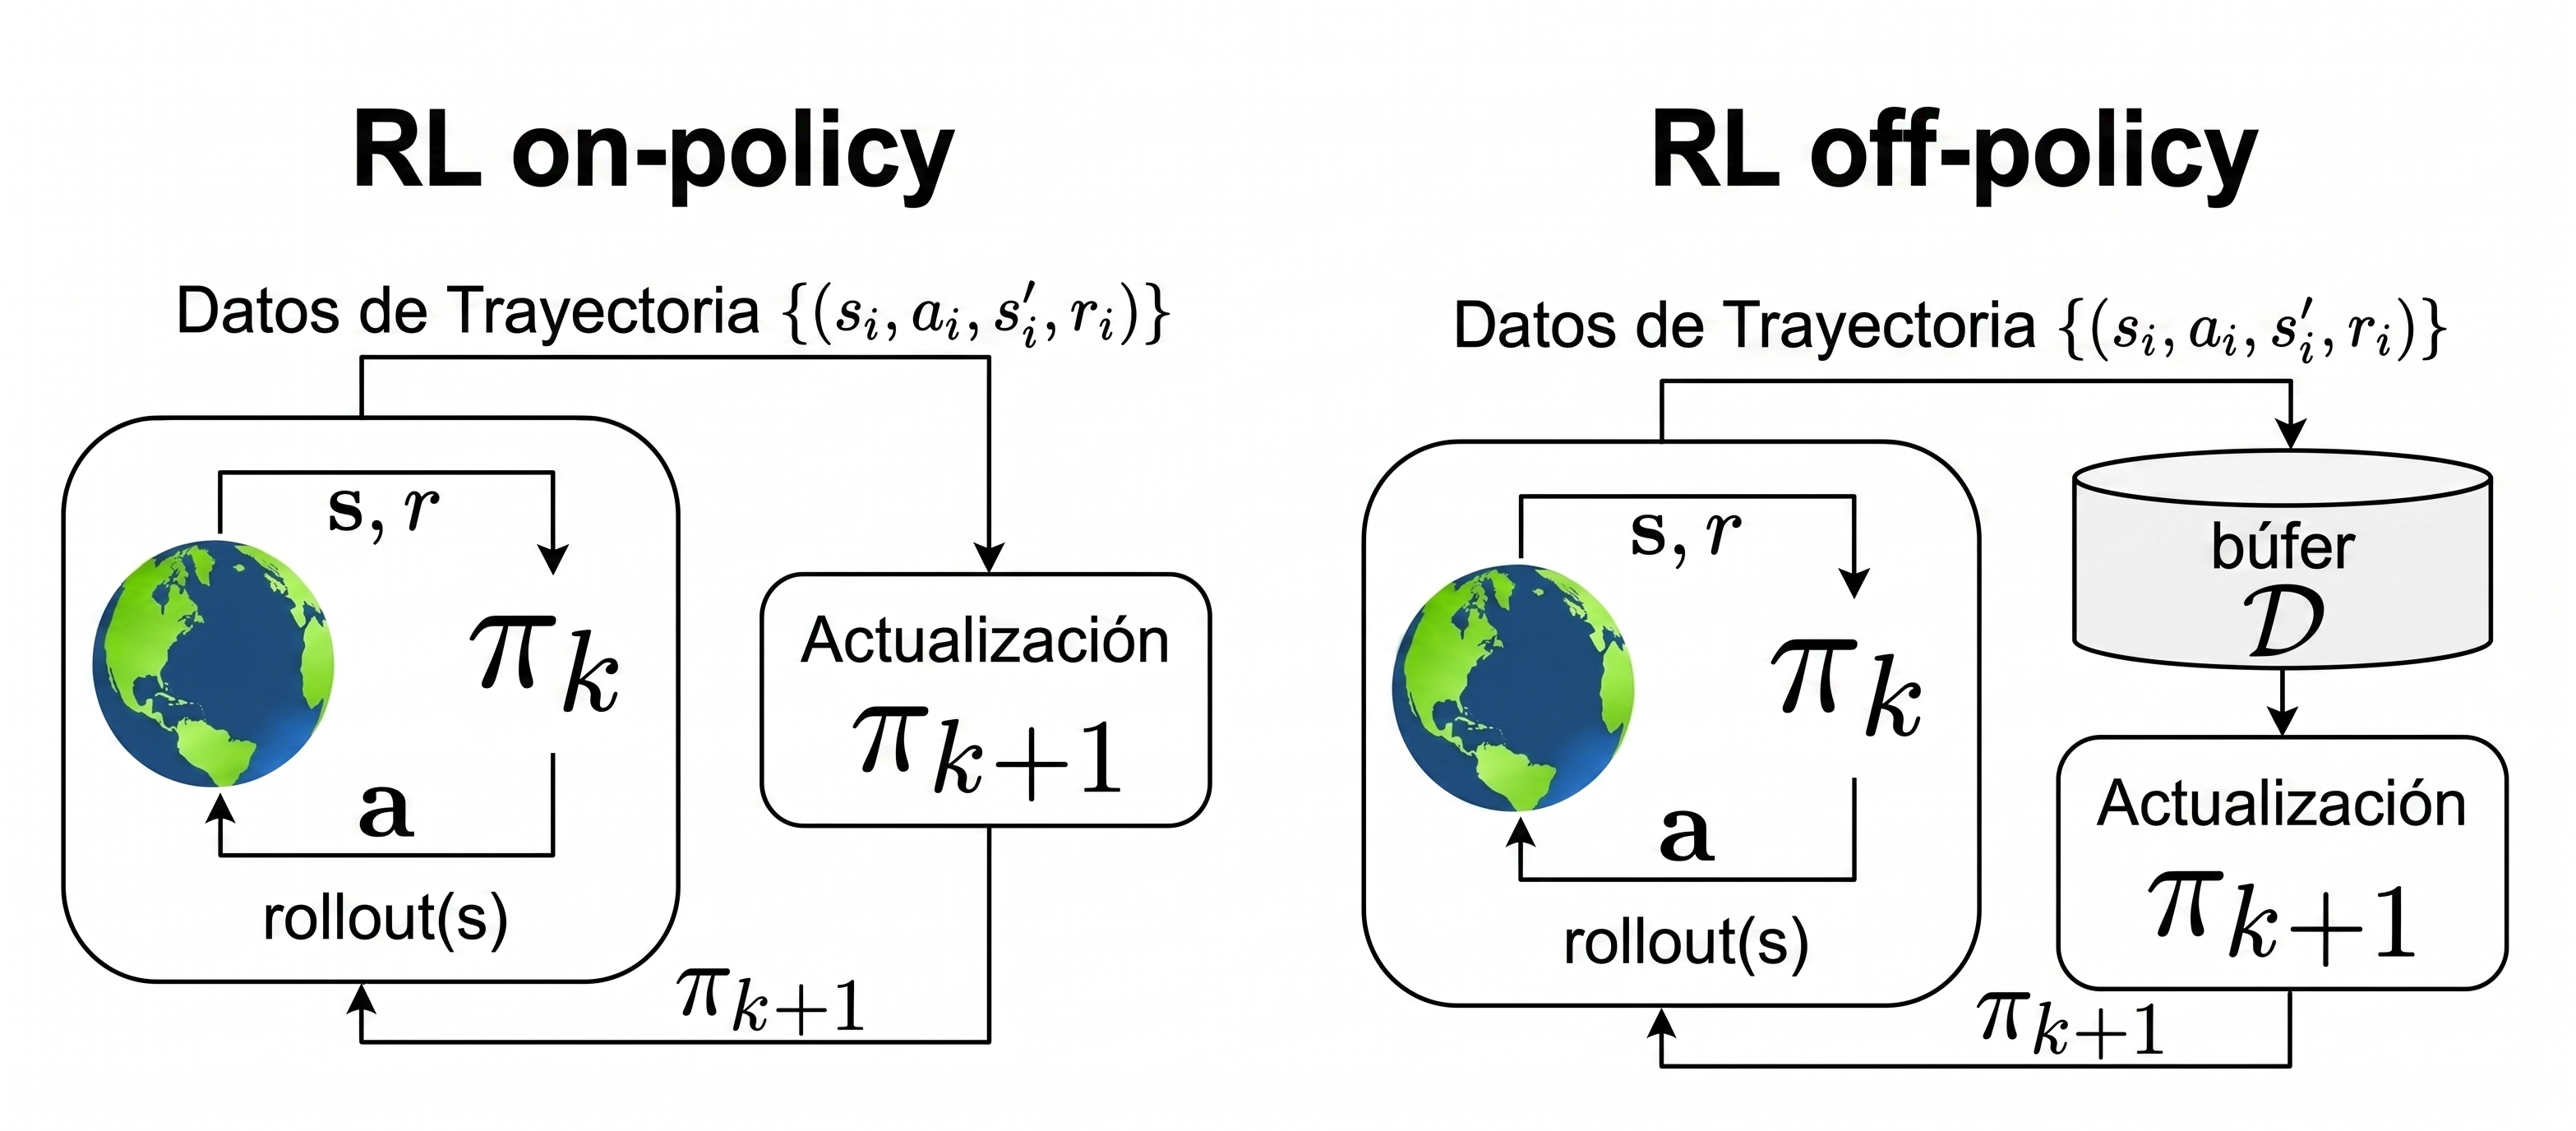
\includegraphics[width=0.55\textwidth]{imaxes/03_marco/on_vs_off.png}
    \caption[On-policy vs off-policy]{Diferencia entre enfoques \gls{on-policy} y \gls{off-policy}. 
    Adaptada de \textit{Offline Reinforcement Learning: Tutorial, Review, and Perspectives on Open Problems}~\cite{DBLP:journals/corr/abs-2005-01643}.}
    \label{fig:on-vs-off}
\end{figure}
 \chapter{Metodología y planificación}
\label{chap:metodologia}

\lettrine{E}{n} este capítulo se describe la metodología seguida durante la
realización del proyecto y su planificación.
Además, se detallan los conjuntos de datos empleados en el
entrenamiento y la evaluación de los modelos.

\section{Enfoque Metodológico}
Al tratarse de un trabajo de investigación con un fuerte componente
experimental, se adoptó un enfoque iterativo e incremental. Esta metodología
permitió construir el sistema de forma gradual, validando cada técnica antes de
incorporar la siguiente y añadiendo valor en cada iteración. A lo largo del
proceso se siguieron los principios de la metodología ágil \textit{Scrum}~\cite{schwaber2020scrum},
basada en ciclos de trabajo cortos y repetitivos
({\glspl{sprint}}) de una duración media de una semana.

Al final de cada iteración se realizaba una evaluación del progreso,
identificando los problemas surgidos y proponiendo soluciones para
continuar con el desarrollo. Esta práctica resultó especialmente útil en un
proyecto con un alto grado de incertidumbre experimental, en el que el resultado de
una técnica condicionaba el diseño de la siguiente. Cada \gls{sprint}
concluía con una reunión con los directores del proyecto, en la
que se revisaban los avances y se establecían los siguientes pasos.

\section{Fases del Proyecto}
El proyecto se inspira fuertemente en el estado del arte (Capítulo~\ref{chap:sota}), con el
que comparte algunos conceptos de diseño (conjunto de acciones, estados, recompensas\dots), pero del que 
difiere en su implementación al probar familias de técnicas muy variadas entre sí, incluyendo algoritmos
no implementados directamente en \textit{Minecraft}, como las \gls{htn}. A continuación se presentan tanto la planificación
inicial como las fases finales en las que se dividió el trabajo.

\subsection{Fases \textit{a priori}}
Antes de comenzar el desarrollo se definieron las siguientes cuatro fases:

\begin{enumerate}
  \item \textbf{Análisis y preparación inicial}: estudio del estado del arte
        sobre agentes en \textit{Minecraft} y familiarización con las herramientas
        (entorno de simulación, comunicación con el agente y
        {\glspl{framework}}).
  \item \textbf{Planificación simbólica}: implementación de la
        \gls{htn} como primera técnica y \textit{baseline} interpretable
        para la comparativa.
  \item \textbf{Aprendizaje por refuerzo}: implementación de un agente de
        refuerzo capaz de resolver la tarea únicamente a partir de la
        observación del entorno.
  \item \textbf{Ejecución y evaluación final}: ejecución de las técnicas,
        configuración necesaria y análisis comparativo de los resultados.
\end{enumerate}

\subsection{Fases \textit{a posteriori}}
En el desarrollo real, el trabajo se dividió en siete iteraciones. Debido a que la aproximación
incremental, el diseño y la realización de cada fase condicionaban la siguiente. Por ejemplo,
la fase de \gls{htn} se usó para generar un conjunto de demostraciones 
que sirvió como base para el \gls{il}, el cual se añadió con posterioridad a la planificación inicial.

\begin{enumerate}
  \item \textbf{Análisis y preparación inicial}: revisión del trabajo previo,
        junto con la familiarización con el
        entorno de simulación y el diseño de la arquitectura general del
        sistema, descrito en el Capítulo~\ref{chap:arquitectura}.
  \item \textbf{Entorno de simulación}: implementación de un entorno
        \gls{gymnasium} comunicado mediante \acrshort{http} con un agente \textit{Mineflayer}~\cite{mineflayer}
        sobre un servidor real de \textit{Minecraft}, con reinicio determinista.
  \item \textbf{Planificación simbólica y generación del \textit{dataset}}:
        implementación del planificador \gls{htn} y de la descomposición de la tarea
        de \gls{woodcutting}, empleando sus ejecuciones como conjunto de
        demostraciones para la fase de \gls{il}.
  \item \textbf{Aprendizaje por imitación}: diseño iterativo y entrenamiento final de una \gls{política} con
        arquitectura de doble cabeza sobre el \textit{dataset} generado por el
        \gls{htn}.
  \item \textbf{Aprendizaje por refuerzo}: diseño iterativo y entrenamiento de una \gls{política} de refuerzo,
        optimizando la arquitectura y los hiperparámetros.
  \item \textbf{Evaluación}: introducción de métricas, definición de una condición de éxito explícita y
        ajuste de la función de recompensa.
  \item \textbf{Resultados y evaluación final}: evaluación de los resultados de todas las implementaciones,
        analizando sus fortalezas y debilidades.
\end{enumerate}

Durante el desarrollo se exploraron además otras dos aproximaciones que
finalmente se descartaron del alcance de la comparativa. La primera fue el uso de
agentes basados en \glspl{llm} mediante el \gls{framework}
\textit{Mindcraft}~\cite{mindcraft2025}, descartada por el elevado coste computacional de ejecutar \glspl{llm} pesados en local. 
La segunda fue un detector visual de árboles
basado en \acrshort{yolo}~\cite{DBLP:conf/cvpr/RedmonDGF16}, descartado por desplazar el objetivo 
hacia un problema de detección de objetos en lugar del aprendizaje de la tarea en sí.

\section{Recursos y limitaciones}
Para el desarrollo del proyecto se emplearon dos equipos: un ordenador de
sobremesa, encargado de ejecutar los entrenamientos, alojar el
servidor de \textit{Minecraft}, ejecutar el agente y el desarrollo general; y un portátil MacBook Air M3,
empleado como equipo secundario. Sus características se resumen en la Tabla~\ref{tab:hardware}
(página~\pageref{tab:hardware}).

\begin{table}[htbp]
  \centering
  \resizebox{\textwidth}{!}{
  \small
  \rowcolors{2}{white}{udcgray!25}
  \begin{tabular}{c|cc}
  \rowcolor{udcpink!25}
  \textbf{Característica} & \textbf{Sobremesa} & \textbf{MacBook Air M3} \\\hline
  \acrshort{cpu} & AMD Ryzen 9 5900X (\num{12}\,C/\num{24}\,T) & Apple M3 (\num{8} núcleos) \\
  \acrshort{ram} & \qty{32}{GB} & \qty{16}{GB} \\
  \acrshort{gpu} & NVIDIA RTX 3060 \qty{12}{GB} & Integrada (\num{10} núcleos) \\
  Uso & Entrenamiento y desarrollo & Equipo complementario \\
  \end{tabular}
  }
  \caption{Equipos empleados en el desarrollo del proyecto.}
  \label{tab:hardware}
\end{table}

La principal limitación de recursos fue el tiempo de entrenamiento. Si bien el
sistema no generaba una gran carga computacional, la ejecución de las acciones
suponía una limitación temporal. El entorno de simulación era el cuello de
botella a la hora de procesar las acciones. Si el agente realiza la acción de
talar y esta requiere \numrange{2}{3} segundos para completarse, en un episodio de \num{100}
pasos el tiempo de ejecución asciende a \numrange{200}{300} segundos. Considerando la ejecución
completa, con \num{300} episodios se alcanzan entre \num{16} y \num{25} horas de entrenamiento, lo
que limita el número de experimentos que se pueden realizar.

La única paralelización posible sería ejecutar varios agentes a la vez o usar
varios equipos simultáneamente, pero no se hizo debido a la limitación de recursos
computacionales disponibles y a la dificultad de coordinar el desarrollo en
varios equipos a la vez.

\section{Conjuntos de Datos}
A diferencia de un problema de clasificación supervisada con conjuntos de datos
estáticos, en este trabajo los datos provienen de la interacción de agentes con
el entorno. Se consideraron dos conjuntos de demostraciones, seleccionando el
primero como conjunto final.

\paragraph{\textit{Dataset} \gls{htn}:} este conjunto de datos de elaboración propia se compone de las 
trayectorias producidas por el agente simbólico al resolver la tarea de
\textit{woodcutting}. Estas trayectorias se registran como pares \textit{OBSERVACIÓN-ACCIÓN} 
(definidos en el Capítulo~\ref{chap:arquitectura}) y conforman el
conjunto de demostraciones de un experto determinista e interpretable. Este
\textit{dataset} permite la comparación entre el comportamiento simbólico y las
técnicas de aprendizaje profundo. Se realiza una pequeña limpieza descartando las 
muestras de acciones poco representativas, quedando un total de \num{118} episodios y
\num{4094} \textit{steps} (\num{4069} tras la limpieza), como se detalla en la Tabla~\ref{tab:datasets} (página~\pageref{tab:datasets}).

\paragraph{\textit{Dataset} MineRL Treechop-v0:} este conjunto de demostraciones humanas~\cite{guss2019minerl}
se compone de \num{210} episodios (todos con éxito) y aproximadamente \num{453000}
\textit{steps}, con una mediana de \num{64} troncos recogidos por episodio.
Su análisis exploratorio reveló que el movimiento de cámara humano (mediana de
\ang{0.75}/\ang{0.90} por \textit{step}) es aproximadamente diez veces
más fino que el paso de cámara de la discretización empleada por los agentes discretos, lo que impide trasladar
directamente las demostraciones humanas a su espacio de acción. Además, el \textit{dataset} humano
presenta limitaciones al ser utilizado fuera del entorno de desarrollo de \textit{MineRL}.
Entre estas limitaciones se encuentran: la estructura de los datos, el formato de las acciones y 
el formato de las observaciones, lo que dificulta su uso directo para el
entrenamiento de agentes en nuestro entorno de simulación. Por último, \textit{MineRL} solo proporciona información
visual, por lo que no permite obtener el vector de estado ni las señales de percepción
(\textit{tree\_visible}, \textit{tree\_distance}) de las que dependen nuestros agentes. 

\begin{table}[htbp]
  \centering
  \resizebox{\textwidth}{!}{
  \small
  \rowcolors{2}{white}{udcgray!25}
  \begin{tabular}{c|cc}
  \rowcolor{udcpink!25}
  \textbf{Propiedad} & \textbf{{htn}} & \textbf{MineRL Treechop-v0} \\\hline
  Origen         & Planificador simbólico (propio) & Demostraciones humanas \\
  Episodios      & \num{118} & \num{210} \\
  \textit{Steps} (bruto)  & \num{4094} & $\sim$\num{453000} \\
  \textit{Steps} (limpio) & \num{4069} & $\sim$\num{453000} \\
  \end{tabular}
  }
  \caption[Conjuntos de datos analizados]{Comparación de los conjuntos de datos analizados en el trabajo.}
  \label{tab:datasets}
\end{table}

Cabe mencionar además que el \gls{framework} de \textit{MineRL} se intentó utilizar, pero actualmente ya no recibe mantenimiento y no es compatible con las versiones actuales de \gls{gymnasium}~\cite{minerl_issue788}. Por otra parte,
este tipo de \textit{datasets} están pensados para ser utilizados dentro de su propio \gls{framework}, 
lo que dificulta su uso en entornos de simulación externos como el empleado en este proyecto.
 \chapter{Arquitectura del Sistema}
\label{chap:arquitectura}

\lettrine{E}{n} este capítulo se describe la arquitectura general del sistema.
Aunque cada técnica utiliza componentes específicos para su funcionamiento,
todas se implementan sobre una misma infraestructura.

Esta decisión permite reutilizar los mecanismos de interacción con el entorno y mantener
condiciones experimentales idénticas entre las tres aproximaciones comparadas.
Las particularidades de cada una se describen en sus respectivos
Capítulos~\ref{chap:iter1}, \ref{chap:iter2} y~\ref{chap:iter3}.

\section{Arquitectura General}
El sistema se organiza en tres capas que se comunican entre sí, como se resume en
la Figura~\ref{fig:arquitectura} (página~\pageref{fig:arquitectura}):
(i) \textbf{Capa de simulación}, un servidor real de \textit{Minecraft};
(ii) \textbf{Capa de agentes}, control del agente y obtención de los estados del mundo;
y (iii) \textbf{Capa de decisión}, comunicación con los modelos de aprendizaje.

\begin{figure}[htbp]
  \centering
  \resizebox{\textwidth}{!}{%
  \begin{tikzpicture}[
    font=\footnotesize, >=Latex,
    box/.style={draw, rounded corners, align=center, minimum width=27mm, minimum height=12mm},
    lbl/.style={font=\scriptsize, align=center, inner sep=2pt},
    legbox/.style={draw, minimum width=6mm, minimum height=3mm, inner sep=0pt}
  ]
    \node[box, fill=udcpink!8]   (serv)  {SERVIDOR DE\\INFERENCIA\\{\scriptsize(\textit{Python} \textbar{} Gym Env)}};
    \node[box, fill=udcgray!8]   (ag)    [right=30mm of serv] {AGENTE\\\textit{MINEFLAYER}};
    \node[box, fill=udcgray!8]   (ag2)   [right=30mm of ag]   {SERVIDOR\\\textit{MINECRAFT}};
    \node[box, fill=ficblue!8] (data)  [above=12mm of ag]   {\textit{DATASET}};
    \node[box, fill=ficblue!8] (visor) [below=14mm of ag]   {VISOR};

    % Servidor de inferencia <-> Agente
    \draw[->] ([yshift=3mm]serv.east) -- node[lbl,above]{HTTP/INFERENCIA} ([yshift=3mm]ag.west);
    \draw[->] ([yshift=-3mm]ag.west)  -- node[lbl,below]{HTTP/ESTADO}     ([yshift=-3mm]serv.east);
    % Agente -> Dataset
    \draw[->] (ag) -- node[lbl,right]{INFO.\ STEP} (data);
    % Agente <-> Agente (agentes concurrentes)
    \draw[->] ([yshift=3mm]ag.east)   -- node[lbl,above]{ACCIONES agente}     ([yshift=3mm]ag2.west);
    \draw[->] ([yshift=-3mm]ag2.west) -- node[lbl,below]{CONOCIMIENTO agente} ([yshift=-3mm]ag.east);
    % Visor -> Agente
    \draw[->] (visor) -- node[lbl,right]{VISIÓN agente} (ag);
    % Visor -> Servidor (entrada visual)
    \draw[->] (visor.west) -| node[lbl,below,pos=0.25]{IMÁGENES} (serv.south);

    % --- LEYENDA (Abajo a la derecha) ---
    \coordinate (legend_pos) at ($(ag2.east |- visor.south) + (0,-12mm)$);
    \node[lbl, anchor=east] (ljs_text) at (legend_pos) {HTN + IL + RL};
    \node[legbox, fill=udcgray!8, left=1.5mm of ljs_text, anchor=east] (ljs) {};

    \node[lbl, left=6mm of ljs, anchor=east] (lpy_text) {IL + RL, No HTN};
    \node[legbox, fill=udcpink!8, left=1.5mm of lpy_text, anchor=east] (lpy) {};
  \end{tikzpicture}
  }
  \caption[Arquitectura general del sistema]{Arquitectura general del sistema. La capa de decisión (\textit{Python}, servidor de
  inferencia para \gls{il} y entorno \gls{gymnasium} para \gls{rl}) se comunica por \acrshort{http} con el
  agente. La \gls{htn} reside por completo en el agente, sin capa de decisión.}
  \label{fig:arquitectura}
\end{figure}

\subsection{Capa de Simulación}
Como se menciona en el Capítulo~\ref{chap:sota}, la mayoría de los trabajos
relacionados con \textit{Minecraft} emplean entornos de simulación propios, basados en versiones
modificadas del juego como \textit{MineRL}~\cite{guss2019minerl}. Sin embargo, muchas
de estas librerías están actualmente abandonadas y presentan problemas de
compilación~\cite{minerl_issue788}, por lo que se opta por un servidor real de
\textit{Minecraft} lanzado en modo \gls{headless} basado en \textit{Paper}\footnote{Una implementación de alto rendimiento del
servidor de \textit{Minecraft}.}~\cite{papermc}.

El mundo utilizado tiene la misma \gls{semilla}\footnote{Código numérico que funciona como plantilla para generar el mapa. Determina dónde
aparecen los biomas, las estructuras, los minerales y el terreno, de modo que la misma \gls{semilla} produce
siempre el mismo mundo.} en todas las iteraciones para evitar mundos donde el agente aparezca en \glspl{bioma} sin árboles
y garantizar el mismo entorno de prueba para todas las técnicas.

Si bien usar el mismo mundo podría limitar la generalización,
se introduce un mecanismo de reinicio con puntos de aparición aleatorios para aportar cierta diversidad de escenarios.

Esta diversidad de escenarios y la reproducibilidad de los episodios se basan en un
reinicio determinista. El reinicio de episodio elimina al agente del mundo y lo teletransporta
a una posición de aparición fija (la primera al entrar al mundo), de modo que cada episodio comienza
con la misma posición dentro del mismo mundo, condición necesaria para que el agente pueda explorar el entorno.
El reinicio de mundo detiene el servidor, borra el mundo y arranca uno nuevo; se puede emplear la misma \gls{semilla}
(para repetir el mismo escenario) o una aleatoria (para generar mundos aleatorios y evaluar la
generalización en distintos entornos).

El agente se conecta al servidor como un jugador mediante
\textit{Mineflayer}~\cite{mineflayer}, una \acrshort{api} en \textit{Node.js}~\cite{nodejs} que
actúa como interfaz entre el código del agente y el mundo de \textit{Minecraft}.

A través de ella se leen las percepciones (posición, orientación,
inventario y bloques cercanos) y se envían las acciones (movimiento,
rotación de cámara, minado e interacción con bloques). La percepción visual
se obtiene de \textit{prismarine-viewer}, un plugin de \textit{Mineflayer} que
renderiza la vista en primera persona del agente en un puerto local (véase el Apéndice~\ref{apx:frame});
\textit{Puppeteer}~\cite{puppeteer} captura esas imágenes y las envía a los
modelos o las guarda en disco para el \textit{dataset} de entrenamiento.

\subsection{Capa de agentes}
Toda la lógica de control gira en torno a una clase base,
\textit{BaseAgent} (Figura~\ref{fig:base-agent}, página~\pageref{fig:base-agent}),
que contiene elementos comunes de los agentes: conexión, punto de aparición en el mundo,
inicialización del visor en primera persona, gestión de errores y desconexión limpia liberando puertos y
recursos. De ella heredan las tres implementaciones de las técnicas:

\begin{figure}[htbp]
  \centering
  \resizebox{\textwidth}{!}{%
  \begin{tikzpicture}[
    font=\footnotesize, >=Latex,
    cls/.style={draw, rounded corners=2pt, align=center, minimum width=26mm, minimum height=10mm},
  ]
    \node[cls, fill=udcpink!8] (base) {\textit{BaseAgent}\\{\scriptsize conexión $\cdot$ spawn $\cdot$ percepción}};
    \node[cls, fill=udcgray!8] (il)  [below=16mm of base] {\textit{ILAgent}};
    \node[cls, fill=udcgray!8] (htn) [left=10mm of il]    {\textit{HTNAgent}};
    \node[cls, fill=udcgray!8] (rl)  [right=10mm of il]   {\textit{RLAgent}};

    % Tronco desde BaseAgent, barra horizontal y flechas hacia cada hijo
    \coordinate (bus) at ($(base.south)+(0,-8mm)$);
    \draw[semithick] (base.south) -- (bus);
    \draw[semithick] (htn.north |- bus) -- (rl.north |- bus);
    \draw[->, semithick] (htn.north |- bus) -- (htn.north);
    \draw[->, semithick] (il.north  |- bus) -- (il.north);
    \draw[->, semithick] (rl.north  |- bus) -- (rl.north);
  \end{tikzpicture}
  }
  \caption[Jerarquía de clases de la capa de agentes]{Jerarquía de clases de la
  capa de agentes. La clase base \textit{BaseAgent} concentra la conexión, el
  punto de aparición y la percepción comunes; de ella heredan \textit{HTNAgent},
  \textit{ILAgent} y \textit{RLAgent}, cada una con su propia lógica de decisión.}
  \label{fig:base-agent}
\end{figure}

\begin{itemize}
  \item \textit{HTNAgent}: ejecuta la \gls{htn}
        directamente, sin intervención externa. Su lógica reside por
        completo en las capas de \textit{Agente} y \textit{Simulación}.
  \item \textit{ILAgent}: en cada paso captura una imagen del visor, la envía al
        servidor de inferencia, recibe la acción predicha (acción discreta
        y delta de cámara) y la ejecuta.
  \item \textit{RLAgent}: actúa como puente entre el entorno \gls{gymnasium} y el agente,
        exponiendo un servidor \acrshort{http} que recibe acciones, las ejecuta y devuelve la
        observación y los eventos.
\end{itemize}

Las tres técnicas comparten la conexión y la percepción, pero difieren en la forma en que deciden la siguiente
acción. Los cambios particulares de las implementaciones se detallan en sus respectivos
Capítulos~\ref{chap:iter1}, \ref{chap:iter2} y~\ref{chap:iter3}.

\subsection{Capa de decisión}
La comunicación entre la capa de decisión (\textit{Python}) y la de agentes (\textit{Node.js}) se
realiza por \acrshort{http} con formatos \acrshort{json}. Se emplean dos canales
según la técnica:

\begin{itemize}
    \item \textbf{Imitación}: el \textit{ILAgent} actúa como cliente de un servidor
        de inferencia \textit{Python} con un \gls{endpoint}
        \textit{/predict}, al que envía la imagen del visor y el vector de estado,
        y del que recibe la acción predicha por el modelo.
    \item \textbf{Refuerzo}: el \textit{RLAgent} levanta un servidor \acrshort{http}
        con tres \textit{endpoints}: \textit{/step}, que recibe una acción,
        la ejecuta y devuelve la nueva observación junto con los eventos
        (bloques rotos, ataque a un árbol, muerte del agente\ldots); \textit{/reset},
        que reinicia el episodio; y \textit{/world\_reset}, que regenera el mundo.
\end{itemize}

\section{Entorno de simulación: Minecraft}
Como ya se describió en el Capítulo~\ref{chap:introduccion}, \textit{Minecraft} es un videojuego
\textit{3D} de mundo abierto en primera persona, basado en bloques y de generación procedimental. La
Figura~\ref{fig:minecraft_view} (página~\pageref{fig:minecraft_view}) muestra la vista en primera persona de
un jugador humano, y la Figura~\ref{fig:3d_axis} (página~\pageref{fig:3d_axis}) muestra el sistema de coordenadas que define su
orientación y posición en el mundo.

\begin{figure}[htbp]
    \centering
    \begin{subfigure}[b]{0.48\textwidth}
        \centering
        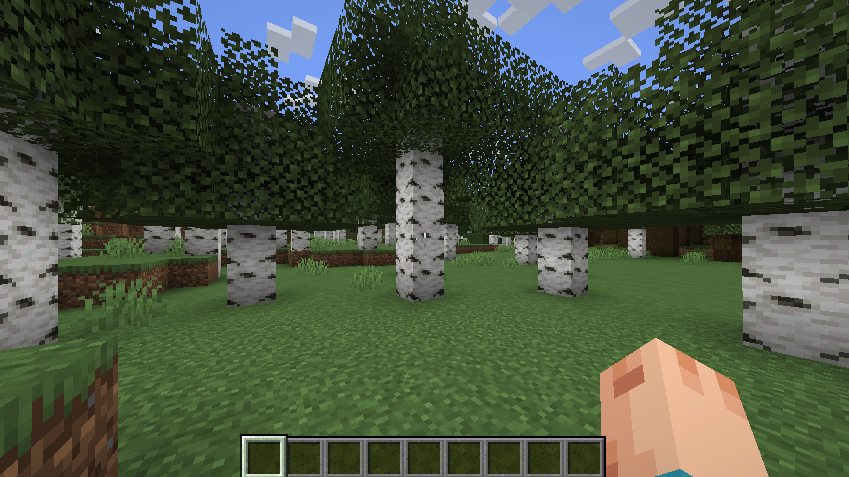
\includegraphics[width=\textwidth]{imaxes/05_arquitectura/minecraft.png}
        \caption{Vista en primera persona de un \gls{bioma} bosque.}
        \label{fig:minecraft_view}
    \end{subfigure}
    \hfill
    \begin{subfigure}[b]{0.48\textwidth}
        \centering
        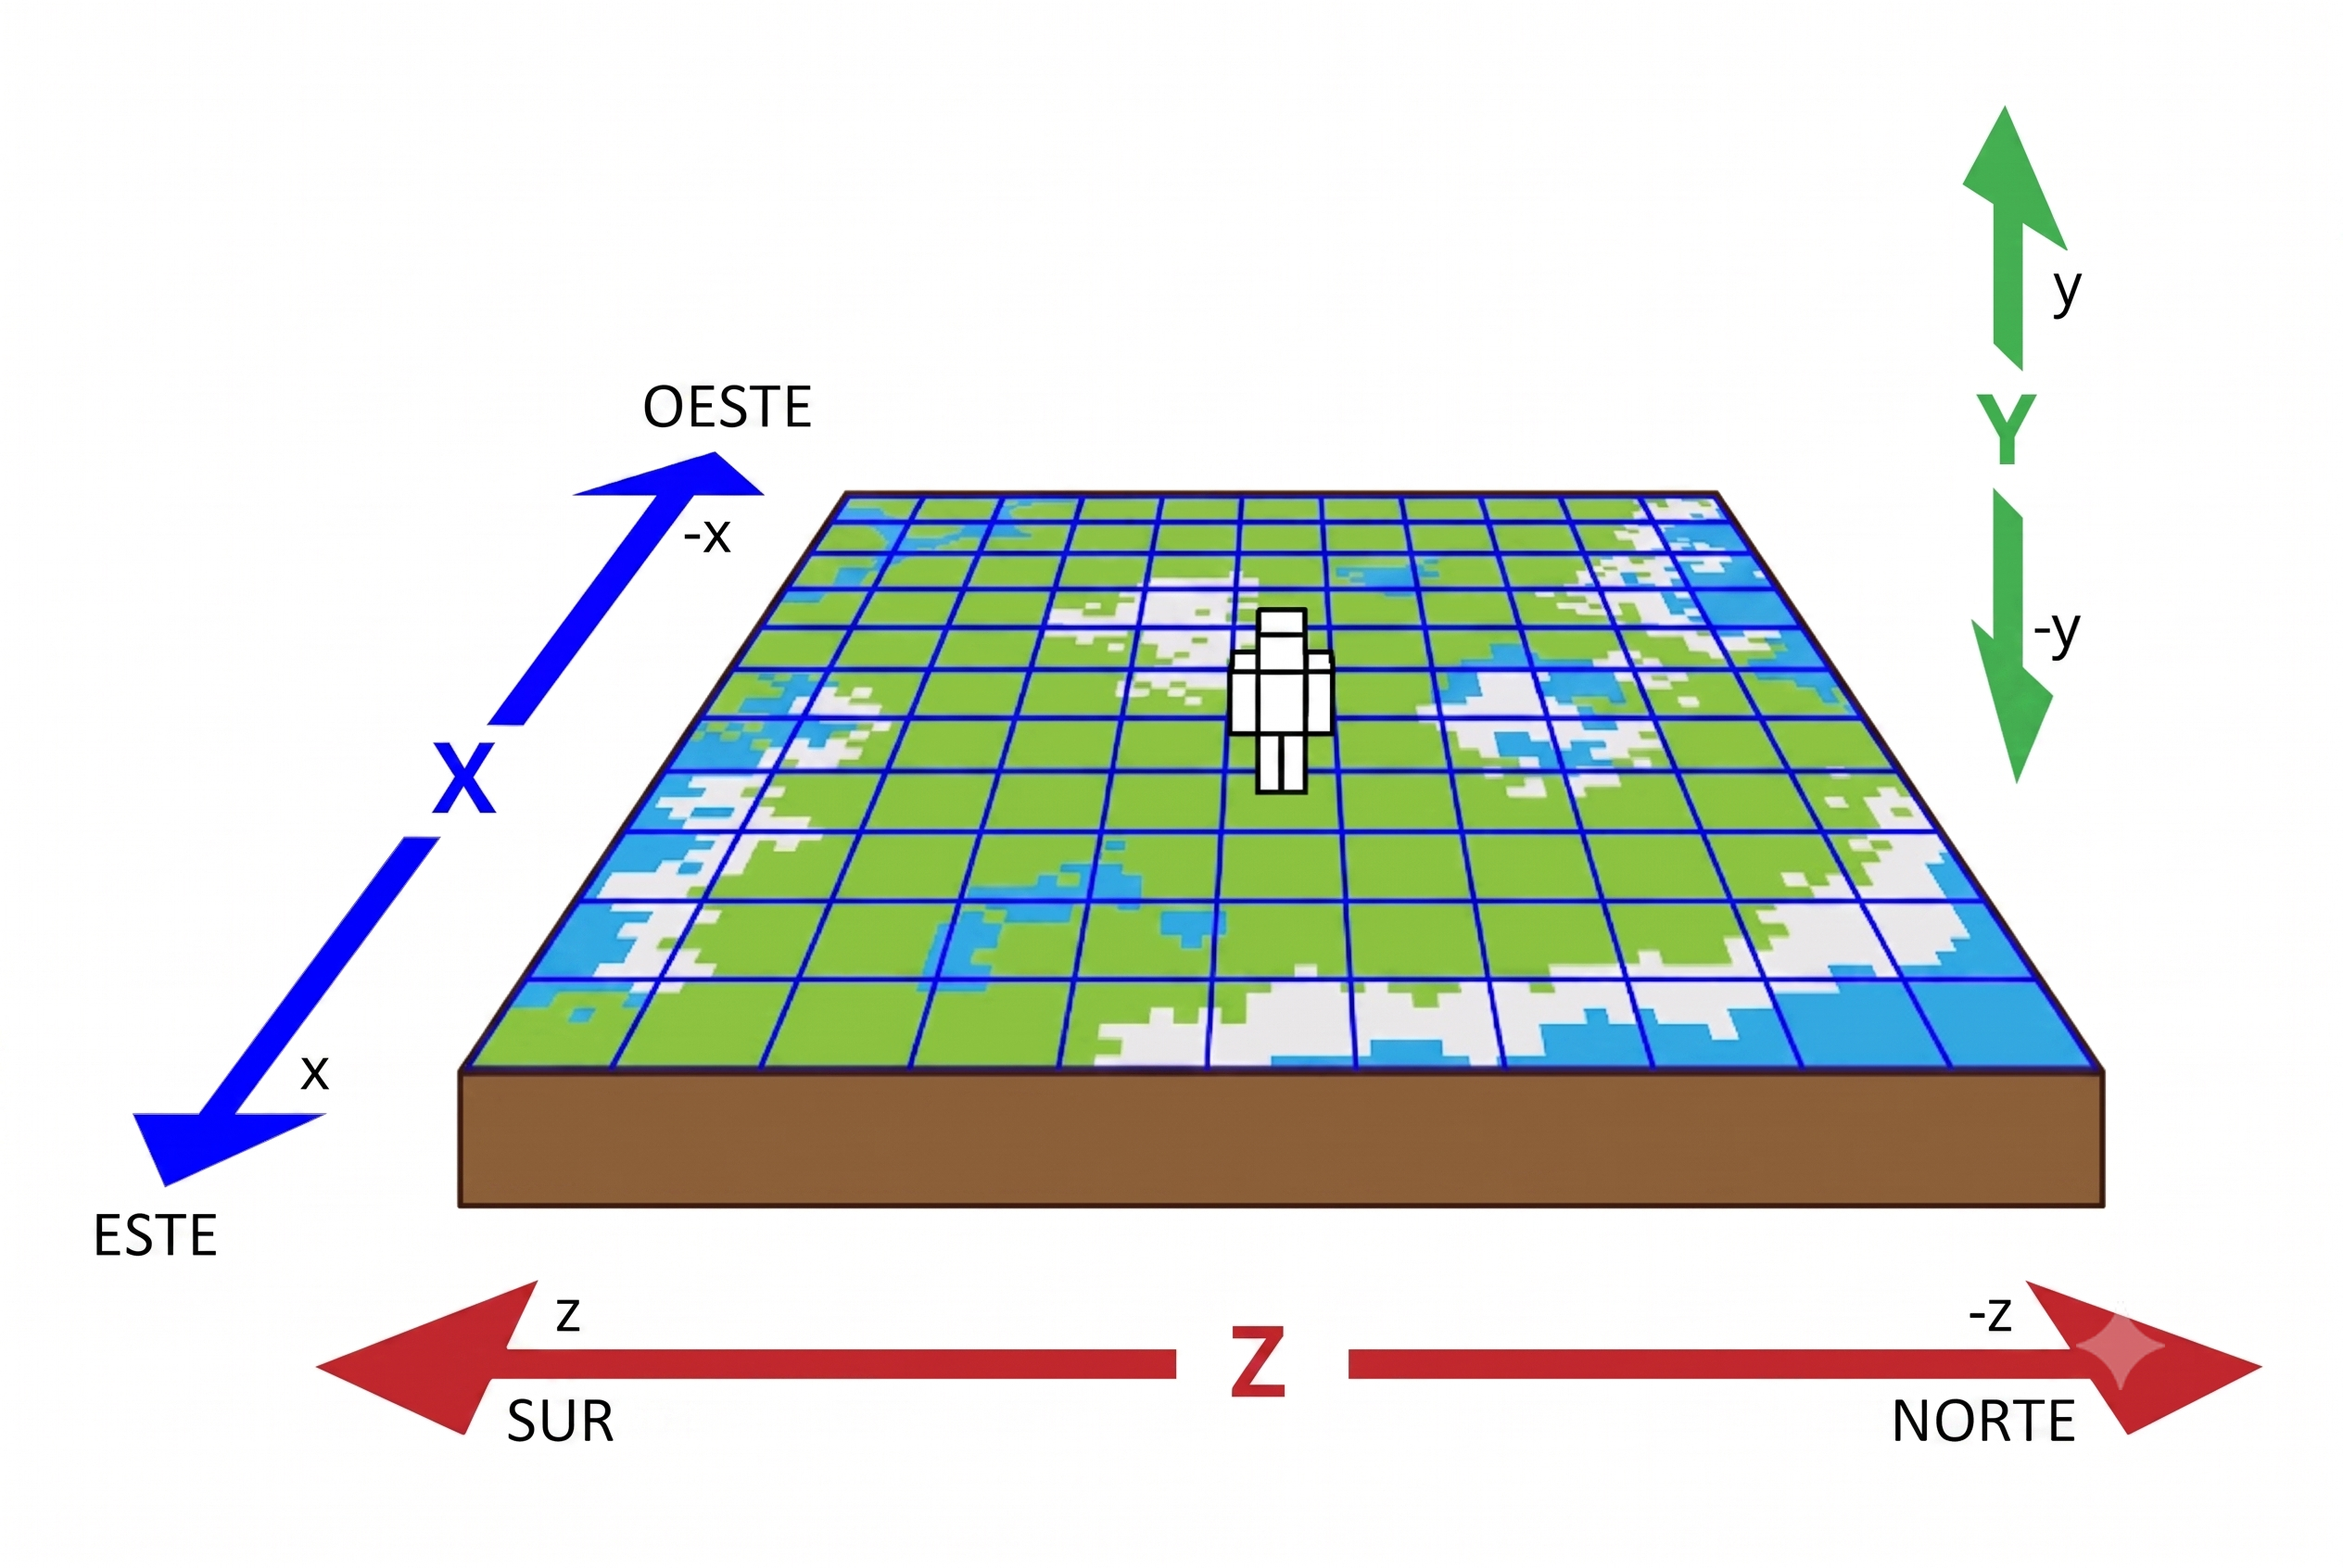
\includegraphics[width=\textwidth]{imaxes/05_arquitectura/3d_axis.png}
        \caption{Sistema de coordenadas 3D del entorno.}
        \label{fig:3d_axis}
    \end{subfigure}
    \caption[Entorno espacial de \textit{Minecraft}]{Entorno espacial de \textit{Minecraft}: vista en primera persona con el
    \gls{hud} activado (izquierda) y representación del sistema de coordenadas (derecha).}
    \label{fig:minecraft_entorno}
\end{figure}

A diferencia de juegos \textit{2D} como \textit{Atari Breakout}~\cite{DBLP:journals/nature/MnihKSRVBGRFOPB15}, el entorno
\textit{3D} introduce una nueva dimensión de complejidad, dificultando así las tareas de navegación,
orientación y percepción visual.

\section{Formulación de la tarea}
La tarea común a todas las técnicas es el \gls{woodcutting}. El agente
debe localizar un árbol, navegar hacia él, talarlo y recoger la madera.

Esta acción es la que realizaría cualquier jugador humano al comenzar a jugar a \textit{Minecraft}, y es el
primer paso de la jerarquía de progresión del juego. Aunque parezca una tarea sencilla desde la perspectiva humana,
presenta una gran dificultad para los agentes autónomos: percepción visual, navegación,
orientación de la cámara, reconocimiento de objetos, recompensa compleja\ldots En las siguientes secciones
se detallan los elementos comunes de la formulación de la tarea, adaptados posteriormente a cada técnica.

\subsection{Espacio de observaciones}
El vector de estado se compone de ocho elementos. Las variables continuas (\textit{yaw}, \textit{pitch},
\textit{dx}, \textit{dz}, \textit{tree\_distance} y \textit{log\_count}) se escalan al rango $[-1,1]$ mediante
límites fijos conocidos del entorno, propios de cada variable: los ángulos \textit{yaw} y \textit{pitch} a
$[-\pi,\pi]$ y $[-\pi/2,\pi/2]$ respectivamente; los desplazamientos del movimiento \textit{dx} y \textit{dz} se recortan a $[-1,1]$
ya que el agente avanza como máximo un bloque por paso; \textit{tree\_distance} a $[0,40]$ bloques (en un
\gls{bioma} de bosque siempre hay un árbol cerca); y \textit{log\_count} a $[0,64]$ (un \gls{stack}
de inventario). Las variables binarias (\textit{tree\_visible} e \textit{is\_looking\_at\_log}) se transforman
a $\{-1,1\}$ para mantener una escala homogénea en las entradas de la red~\cite{DBLP:series/lncs/LeCunBOM12}.
La Tabla~\ref{tab:obs-space} (página~\pageref{tab:obs-space}) resume los elementos del vector de estado.

\begin{table}[htbp]
  \centering
  \resizebox{\textwidth}{!}{%
  \small
  \rowcolors{2}{white}{udcgray!25}
  \begin{tabular}{c|c|c}
  \rowcolor{udcpink!25}
  \textbf{Componente} & \textbf{Rango} & \textbf{Descripción} \\\hline
  \textit{yaw}               & $[-\pi,\pi]$     & Orientación horizontal de la cámara (rad) \\
  \textit{pitch}             & $[-\pi/2,\pi/2]$ & Orientación vertical de la cámara (rad) \\
  \textit{dx}                & $[-1,1]$         & Desplazamiento en X respecto al paso anterior \\
  \textit{dz}                & $[-1,1]$         & Desplazamiento en Z respecto al paso anterior \\
  \textit{tree\_visible}     & $\{-1,1\}$       & Indicador de árbol visible en el cono de visión \\
  \textit{tree\_distance}    & $[0,40]$         & Distancia al árbol visible más cercano \\
  \textit{log\_count}        & $[0,64]$         & Troncos acumulados en el inventario \\
  \textit{is\_looking\_at\_log} & $\{-1,1\}$    & Indicador de cursor apuntando a un tronco \\
  \end{tabular}%
  }
  \caption[Elementos del vector de estado]{Elementos del vector de estado.}
  \label{tab:obs-space}
\end{table}

La posición absoluta $(x, y, z)$ se excluye del vector de estado de los agentes
para favorecer la generalización. Con coordenadas absolutas, el agente podría tender a memorizar posiciones
concretas del mundo en lugar de aprender a talar. En su lugar se conservan los
desplazamientos entre pasos $(dx, dz)$, que aportan información útil.
Del mismo modo, solo se conserva el desplazamiento horizontal $(dx, dz)$ y se omite el vertical $(dy)$.
En el \gls{bioma} utilizado el movimiento vertical es prácticamente nulo, por lo que aportaría un
componente casi constante y sin información, al ser la mayoría de los valores 0. Además, la entrada visual 
codifica de manera implícita la altura del agente respecto a su entorno, 
aportando un contexto espacial mucho más rico y útil que la inclusión de una coordenada vertical en el vector de estado.
Cuando se habilita la entrada visual, además del vector de estado, la red recibe una imagen \acrshort{rgb} de
\num{128} $\times$ \num{128} píxeles capturada del visor en primera persona.
En ambos casos se admite el \gls{frame-stacking}, repetir las últimas
$k$ observaciones, para dar información temporal a la red.

\subsection{Espacio de acciones}
El espacio de acciones utilizado consta de siete acciones recogidas en la
Tabla~\ref{tab:action-space} (página~\pageref{tab:action-space}).
La cámara se discretiza en giros fijos: \qty{0.15}{rad} ($\approx$ \ang{8.6})
en horizontal y \qty{0.10}{rad} ($\approx$ \ang{5.7}) en vertical. Se utiliza esta
granularidad para conseguir un cambio de estado real, sin que el agente gire la cámara manteniéndose en el mismo estado.

\begin{table}[htbp]
  \centering
  \resizebox{\textwidth}{!}{%
  \small
  \rowcolors{2}{white}{udcgray!25}
  \begin{tabular}{c|c}
  \rowcolor{udcpink!25}
  \textbf{Acción} & \textbf{Efecto} \\\hline
  \textit{attack}                & Minar el bloque apuntado por el cursor \\
  \textit{move\_forward\_sprint} & Avanzar corriendo \\
  \textit{move\_forward\_jump}   & Avanzar corriendo con salto \\
  \textit{camera\_right}         & Girar la cámara a la derecha \\
  \textit{camera\_left}          & Girar la cámara a la izquierda \\
  \textit{camera\_up}            & Subir la cámara \\
  \textit{camera\_down}          & Bajar la cámara \\
  \end{tabular}%
  }
  \caption[Espacio de acciones discreto]{Espacio de acciones discreto.}
  \label{tab:action-space}
\end{table}

\subsection{Condiciones de terminación y éxito}
Un episodio puede finalizar de tres formas. La primera es el \textbf{éxito}: recoger al menos el
número de troncos objetivo $k$ y, además, haber roto al menos
un tronco durante el episodio. Esta segunda condición previene un comportamiento espurio
donde el agente recoge troncos de episodios anteriores sin talar nuevos árboles.

La segunda forma es la \textbf{terminación anticipada}, que se dispara si el agente muere o si la
recompensa acumulada cae por debajo de un umbral, cortando episodios sin progreso. Al ser un final
real de la tarea, se deja el valor del estado siguiente a cero.

La última forma es el \textbf{truncamiento}, al alcanzar el número máximo de
pasos por episodio. A diferencia de la terminación, el valor del estado siguiente no es cero,
lo que indica al agente que el episodio aún podría continuar.

\subsection{Percepción del entorno}
El componente principal de la percepción es la detección de árboles. Si bien el agente
podría obtener un conocimiento omnisciente del mundo a través de la \acrshort{api} de \textit{Mineflayer} (conociendo la
posición exacta de cualquier bloque, enterrado o tras un muro), se limita
la información que recibe para simular lo máximo posible la percepción de un jugador humano.

Para ello, la búsqueda de troncos se restringe al
\gls{fov} del agente, evitando información sobre objetos
que no podría ver. Además, para percibir un objeto el agente debe tener una línea de
visión directa hacia él.

La detección comienza con la función \textit{findBlocks} de \textit{Mineflayer}, que devuelve
las posiciones de los bloques de un tipo dado dentro de un radio fijo (por defecto, \num{32} bloques)
alrededor del agente. Los bloques devueltos por la función vienen ordenados por cercanía al agente. Sobre esos candidatos se aplica un
filtro en tres etapas, devolviendo el primer bloque que las supera todas:

\begin{enumerate}
  \item \textbf{Cara expuesta}: el bloque debe tener al menos una cara al aire. Esto
        asegura que el bloque es visible y accesible directamente.
  \item \textbf{Cono de visión}: el bloque debe estar dentro del campo de visión
        del agente, cono de \ang{90} en horizontal y
        \ang{60} en vertical respecto a la orientación (\textit{yaw}, \textit{pitch})
        del agente.
  \item \textbf{Línea de visión}: se traza un \gls{raycast} (línea proyectada desde un punto fijo en una dirección concreta)
        desde los ojos del agente hasta el bloque, el cual debe alcanzarse sin chocar previamente con otro bloque sólido
        (elementos como el agua no bloquean la visión).
\end{enumerate}

De este modo, el agente solo conoce los árboles que un jugador podría realmente
ver en ese instante.

\subsection{Reproducibilidad}
La reproducibilidad del sistema se basa en el uso del mismo mundo y \gls{semilla} en todas las iteraciones y en los
reinicios deterministas a una posición de aparición fija. Así, todas las técnicas se entrenan y evalúan bajo
idénticas condiciones, variando únicamente en la posición inicial al generar el mundo, lo que garantiza que las comparaciones 
entre las familias de algoritmos del Capítulo~\ref{chap:discusion-resultados} sean justas.
 \chapter{Iteración I - Agente HTN}
\label{chap:iter1}

\lettrine{E}{n} esta primera iteración, se aborda la planificación simbólica
usando un planificador jerárquico de tareas (\gls{htn}), que sirve de base
para la comparación con el resto de algoritmos gracias a su carácter determinista 
y explicable.

Como resultado de esta iteración se obtienen dos elementos: un agente
que actúa como \textit{baseline} frente a las técnicas de
aprendizaje, y un \textit{dataset} propio de demostraciones generado a partir de
sus ejecuciones para entrenar en el Capítulo~\ref{chap:iter2}.

\section{Diseño}
La tarea objetivo \gls{woodcutting} consiste en la recolección de $k$ troncos de un tipo específico de madera.
Esta tarea objetivo se descompone en una tarea compuesta que se
resuelve aplicando repetidamente una secuencia de primitivas (Figura~\ref{fig:htn-tree}, página~\pageref{fig:htn-tree}).

\begin{figure}[htbp]
  \centering
  \begin{forest}
    for tree={
      font=\footnotesize, grow'=0, folder, rounded corners, draw,
      edge={-, semithick}, l sep=4mm, s sep=1.2mm, anchor=west,
      inner sep=2.5pt,
    },
    compuesta/.style={fill=blue!8},
    primitiva/.style={fill=green!12},
    recup/.style={fill=red!10},
    [{Recolectar $k$ troncos \textit{(post-cond.: hasItem)}}, compuesta
      [{Obtener tipo de madera \textit{(obtainWoodType)}}, primitiva]
      [{Talar tronco --- repetir hasta $k$}, compuesta
        [{Buscar árbol visible en cono \gls{fov} \textit{(findNearestVisibleBlock)}}, primitiva]
        [{Explorar si no hay árbol \textit{(exploreRandom)}}, recup]
        [{Ir al árbol \textit{(moveToBlock)}}, primitiva]
        [{Talar el tronco completo \textit{(mine)}}, compuesta
          [{Talar y recoger el bloque base \textit{(collectBlock)}}, primitiva]
          [{Moverse y talar el resto \textit{(mineTreeTrunk)}}, primitiva]
        ]
      ]
    ]
  \end{forest}
  \caption[Árbol de descomposición de la tarea de woodcutting]{Árbol de
  descomposición \gls{htn} de la tarea de \gls{woodcutting}. La tarea compuesta
  se descompone en una primitiva de selección de madera y en una
  tarea compuesta de tala que se repite hasta conseguir los $k$ troncos. Las tareas
  \textbf{compuestas} se muestran en \textbf{azul}, las \textbf{primitivas} en \textbf{verde} 
  y la \textbf{recuperación} en \textbf{rojo}.}
  \label{fig:htn-tree}
\end{figure}

Cada tarea se define mediante: una \textbf{pre-condición}, estado del mundo antes de la ejecución;
una \textbf{post-condición}, estado del mundo después de la ejecución; y un \textbf{método}, forma de resolver la tarea usando 
una secuencia de subtareas (primitivas u otras compuestas). 
Estas restricciones son las que otorgan al agente su carácter \textbf{determinista} (ante el
mismo estado toma siempre la misma decisión) e \textbf{interpretable} (cada acción
corresponde a una regla).

La condición de éxito de la tarea de \gls{woodcutting} es tener $k$ troncos en
el inventario. Al ser una tarea objetivo, no se ejecuta de forma directa, sino que se
descompone en la tarea compuesta de talar un árbol, que se repite hasta alcanzar
los $k$ troncos. Talar un árbol implica, a su vez, varios pasos: localizar un tronco
dentro del \gls{fov} (y, si no hay ninguno, explorar el mundo hasta que aparezca
uno), desplazarse hasta él y, finalmente, talar el tronco completo. Cada uno de estos
pasos se descompone de nuevo hasta llegar a primitivas como mover la cámara o minar un bloque.

Al ser una de las primeras tareas a realizar en \textit{Minecraft}, la tarea \gls{woodcutting} no presenta realmente pre-condiciones, ya que el agente puede empezar a talar en cualquier momento. Sin embargo, en tareas posteriores como la obtención de un pico de hierro es necesario que el agente tenga las herramientas adecuadas (véase el Apéndice~\ref{apx:htn-iron-decomp}).

\section{Tareas Primitivas}
Las tareas primitivas que componen la tarea de \gls{woodcutting} se recogen
en la Tabla~\ref{tab:htn-primitivas} (página~\pageref{tab:htn-primitivas}). Cada primitiva se traduce en una acción
básica realizable en \textit{Minecraft} (moverse, minar, mover la cámara\dots) y 
se apoya en la \acrshort{api} de \textit{Mineflayer} descrita en el Capítulo~\ref{chap:arquitectura}.

\begin{table}[htbp]
  \centering
  \resizebox{\textwidth}{!}{%
  \small
  \rowcolors{2}{white}{udcgray!25}
  \begin{tabular}{c|c}
  \rowcolor{udcpink!25}
  \textbf{Primitiva} & \textbf{Función} \\\hline
  \textit{obtainWoodType}          & Determinar el tipo de madera  \\
  \textit{findNearestVisibleBlock} & Localizar el tronco visible más cercano (\gls{fov}) \\
  \textit{moveToBlock}             & Navegar al bloque mediante un \gls{pathfinder} \\
  \textit{collectBlock}            & Obtener un bloque y recogerlo \\
  \textit{mineTreeTrunk}           & Talar una secuencia de bloques \\
  \textit{exploreRandom}           & Explorar si no hay árbol visible (recuperación) \\
  \end{tabular}
  }
  \caption[Primitivas del agente simbólico para la tarea de woodcutting]{Primitivas del agente simbólico para la tarea de \textit{woodcutting}.}
  \label{tab:htn-primitivas}
\end{table}

\paragraph{Selección del tipo de madera:}
utilizando la \acrshort{api} de \textit{Mineflayer}
se identifica el \gls{bioma} y, mediante un mapeo predefinido, se determina el tipo de madera objetivo a talar
(por ejemplo, \textit{forest} $\rightarrow$ \textit{oak\_log}); si el bioma no está mapeado, se recurre a una
búsqueda visual de los tipos de tronco más comunes en el entorno. Si no hay
madera visible al alcance, la tarea falla en lugar de consultar la posición
omnisciente de los bloques, en coherencia con la restricción de percepción del
Capítulo~\ref{chap:arquitectura}. 

\paragraph{Búsqueda de Bloques en el Cono de Visión:}
la localización de troncos reutiliza el mismo mecanismo de percepción definido en
el Capítulo~\ref{chap:arquitectura}. La búsqueda se restringe al 
\gls{fov} del agente y exige línea de visión directa, de modo que el agente solo
considera los árboles que un jugador humano vería. La primitiva de
talar usa esta búsqueda para evitar información del mundo fuera del \gls{fov}.

\paragraph{Tala del Tronco:}
una vez localizado el bloque, la tala no vuelve a invocar
la búsqueda por \gls{fov} para los bloques superiores. En su lugar,
\textit{mineTreeTrunk} recorre verticalmente la posición
ya conocida: mina el bloque en $(x,\,y{+}1,\,z)$, comprueba si el bloque
en $(x,\,y{+}n,\,z)$ es del mismo tipo de tronco, y así sucesivamente hasta
que el tipo de bloque cambia. Esta estrategia permite talar un árbol completo
sin necesidad de reposicionarse ni relanzar el \gls{pathfinder} para cada bloque.

\paragraph{Exploración de Recuperación:}
cuando la búsqueda en el \gls{fov} no encuentra ningún árbol,
el agente no puede determinar si existe madera en el mundo o si simplemente no
es visible desde su posición actual. En este caso se activa \textit{exploreRandom},
que elige una dirección aleatoria y pide al \gls{pathfinder} avanzar hasta \num{30} bloques
en esa dirección, permaneciendo en la superficie
para evitar posiciones subterráneas donde no se encuentra madera. Durante la exploración, se
comprueba cada \qty{500}{ms} si ha aparecido algún tronco en el \gls{fov}; si es así, la
exploración se interrumpe y se retoma la tala.

\paragraph{Progresión y Recuperación de Fallos:}
la ejecución de cada tarea contiene una 
lógica de recuperación (Figura~\ref{fig:htn-recovery}, página~\pageref{fig:htn-recovery}). 
Antes de actuar se comprueba la post-condición;
mientras no se cumpla, se ejecuta el método de la tarea hasta un máximo de $N$
intentos. Si un intento lanza un error (por ejemplo, el objetivo ha desaparecido), 
se dispara un mecanismo de recuperación: una acción de recuperación
específica de la tarea o, si no existe, una exploración aleatoria del entorno
para reposicionar al agente antes de reintentar. 
Si el agente se queda sin intentos, la tarea se aborta y se propaga el fallo a la tarea padre,
o bien, se detiene la ejecución si es la tarea raíz, marcando la ejecución como fallida.

\begin{figure}[htbp]
  \centering
  \resizebox{\textwidth}{!}{%
  \begin{tikzpicture}[
    font=\footnotesize, >=Latex,
    proc/.style ={draw, rounded corners, align=center, minimum width=26mm, minimum height=8mm, fill=ficblue!8},
    dec/.style  ={draw, diamond, aspect=2.4, align=center, inner sep=1pt, fill=udcgray!8},
    term/.style ={draw, rounded corners, align=center, minimum width=24mm, minimum height=8mm},
  ]
    \node[dec] (post) {¿Post-cond.?};
    \node[proc] (met) [right=12mm of post] {Ejecutar método};
    \node[dec]  (int) [right=12mm of met] {¿Quedan intentos?\\{\scriptsize(máx.\ $N$)}};
    
    \node[term, fill=udcpink!25]  (abort) [right=12mm of int] {ABORTAR};
    \node[term, fill=green!12] (comp) [above=12mm of post] {COMPLETADO};
    \node[term, fill=udcgray!8] (padre) [below=10mm of abort] {Tarea padre};
    
    \node[proc, fill=udcpink!8] (rec)   [below=12mm of int]  {Recuperación\\{\scriptsize exploración, atascos}};

    \draw[->] (post) -- node[left]{sí} (comp);
    \draw[->] (post) -- node[above]{no} (met);
    \draw[->] (met)  -- node[above]{error} (int);
    \draw[->] (int)  -- node[above]{no} (abort);
    \draw[->] (int)  -- node[right]{sí} (rec);
    \draw[->] (abort) -- (padre);

    \path (rec.south) -- ++(0,-6mm) coordinate (ret_y);
    
    \draw[-] (rec.south) |- (met.south |- ret_y);
    \draw[->] (met.south) -- node[right]{éxito} (met.south |- ret_y);
    \draw[->] (met.south |- ret_y) -| (post.south);
    
  \end{tikzpicture}
  }
  \caption[Bucle de ejecución de una tarea]{Bucle de ejecución de una tarea
  (\textit{runSmartTask}) del \gls{htn}. Antes de cada intento se comprueba la post-condición; mientras no
  se cumpla, se ejecuta el método de la tarea. Si un intento falla, se dispara un mecanismo de
  recuperación (una acción específica o una exploración aleatoria) y se reintenta, hasta un
  máximo de $N$ intentos. Si se agotan, la tarea se aborta y propaga el fallo a la tarea padre.}
  \label{fig:htn-recovery}
\end{figure}


Se añaden dos prevenciones extra debido a las limitaciones de la simulación. La primera consiste en una comprobación periódica de
la posición del agente mientras el \gls{pathfinder} está activo; si no avanza lo suficiente durante varias
muestras consecutivas (por ejemplo, si el agente se queda atascado), se reinicia la navegación. 
La segunda es un \textit{timeout} global por episodio que limita la
duración máxima de una ejecución para evitar bucles infinitos.

\section{Generación del Dataset de Demostraciones}
\label{sec:dataset-htn}
Al comenzar la implementación del agente de imitación (Capítulo~\ref{chap:iter2})
surgió la necesidad de un conjunto de demostraciones de un experto. Una de las opciones
sería reutilizar un \textit{dataset} público como \textit{MineRL}~\cite{guss2019minerl},
cuyo subdataset \textit{Treechop-v0} aborda precisamente la misma tarea. Sin
embargo, su uso resulta imposible en este trabajo por los motivos mencionados en el 
Capítulo~\ref{chap:metodologia}.

Por todo ello, en lugar de adaptar un \textit{dataset} ajeno se genera uno propio
ejecutando el agente \gls{htn} sobre el mismo entorno en el que se evalúan las técnicas.
Al compartir exactamente el mismo entorno, espacio de acciones y espacio de observación
que el agente de imitación, las demostraciones no necesitan ninguna conversión y
sus etiquetas coinciden con el conjunto de acciones del modelo. Esto
garantiza la coherencia entre el experto y el aprendiz y elimina el desajuste de
formato y granularidad de \textit{datasets} externos.

Durante la ejecución se almacenan pares
\textit{OBSERVACIÓN-ACCIÓN} que conformarán el \textit{dataset}. A intervalos regulares se captura un \textit{frame} 
que combina la imagen del visor en primera persona (véase el Apéndice~\ref{apx:frame}), el vector de estado del agente
de la Tabla~\ref{tab:obs-space} (página~\pageref{tab:obs-space}) y la acción que está ejecutando en ese
instante. Cabe destacar que no se incluyen los movimientos de la cámara como acciones discretas, ya que el agente 
los realiza sobre posiciones absolutas del mundo; es decir, no emplea acciones como \textit{camera\_right}, 
sino que orienta su visión directamente mediante funciones como \textit{lookAt(x,y,z)}.
Los \textit{frames} sin acción se descartan (por ejemplo, los capturados durante el tiempo de inicialización, 
donde el agente aún no interactúa con el entorno).
La estructura final de estos \textit{frames} se detalla en la Tabla~\ref{tab:dataset-frame} (página~\pageref{tab:dataset-frame}).

\begin{table}[htbp]
  \centering
  \resizebox{\textwidth}{!}{%
  \small
  \rowcolors{2}{white}{udcgray!25}
  \begin{tabular}{c|c|c}
  \rowcolor{udcpink!25}
  \textbf{Campo} & \textbf{Tipo / Rango} & \textbf{Descripción} \\\hline
  \textit{image}                & PNG               & Vista en primera persona del visor \\
  \textit{x, y, z}              & float (bloques)   & Posición del agente \\
  \textit{yaw, pitch}           & float (rad)       & Orientación de la cámara \\
  \textit{action}               & categórica        & Acción discreta ejecutada en el \textit{frame} \\
  \textit{dyaw, dpitch}         & float (rad)       & Desplazamiento de cámara respecto al \textit{frame} anterior \\
  \textit{tree\_visible}        & $\{0, 1\}$        & Árbol dentro del \gls{fov} \\
  \textit{tree\_distance}       & float (bloques)   & Distancia al árbol visible más cercano \\
  \end{tabular}
  }
  \caption[Estructura de los \textit{frames} del dataset.]{Estructura de los \textit{frames} del \textit{dataset} de demostraciones
  generado por el \gls{htn}. La posición absoluta se guarda para calcular el desplazamiento entre \textit{frames} posteriormente.}
  \label{tab:dataset-frame}
\end{table} 

La distribución de acciones del \textit{dataset}, ilustrada en la Figura~\ref{fig:dataset-clases} (página~\pageref{fig:dataset-clases}), está desbalanceada.
Esto se debe a que el agente simbólico dispone de información completa del entorno a través de la \acrshort{api},
lo que le permite actuar de forma muy eficiente. Por ejemplo, conoce la posición exacta de los árboles y, 
mediante el uso del \gls{pathfinder}, calcula rutas óptimas que rara vez incluyen movimientos laterales o hacia atrás. 
Como consecuencia, aunque el espacio de acciones contiene acciones como saltar, moverse a la derecha o moverse a la izquierda, 
el agente solo ejecuta las más eficientes para completar la tarea. Este comportamiento provoca que ciertas 
acciones aparezcan con muy poca frecuencia en el \textit{dataset}, lo que motiva el descarte de las clases menos representadas.

\begin{figure}[htbp]
  \centering
  \resizebox{\textwidth}{!}{%
  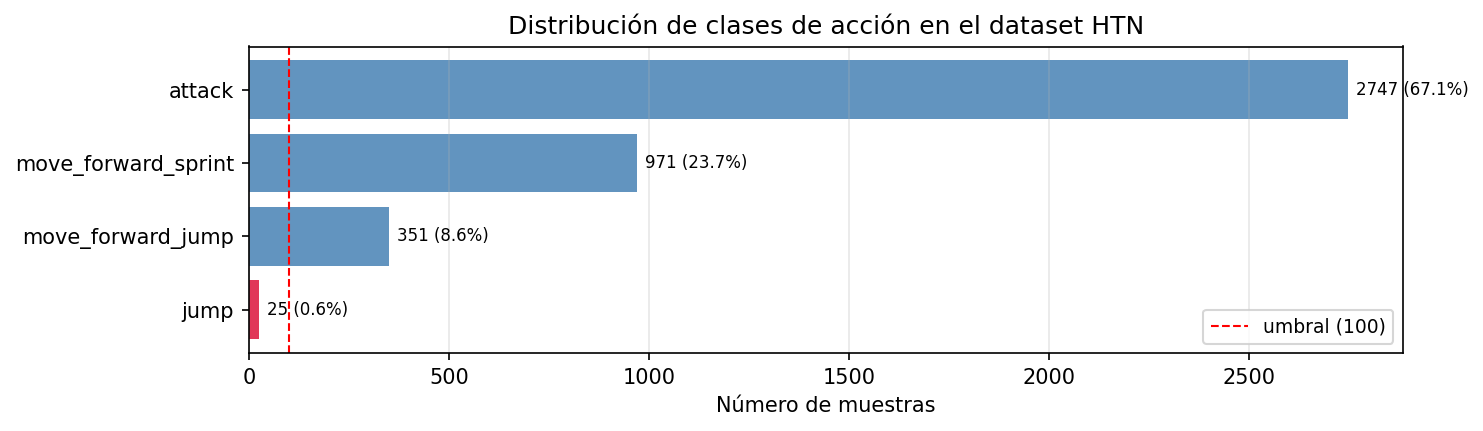
\includegraphics[width=1\textwidth]{imaxes/06_htn/dataset_clases.png}
  }
  \caption[Distribución de clases de acción en el dataset HTN]{Distribución de
  las clases de acción en el \textit{dataset} de demostraciones generado por el agente
  simbólico tras \num{118} ejecuciones.}
  \label{fig:dataset-clases}
\end{figure}

El registro de la acción discreta y la variación de la cámara es lo que
permite entrenar una arquitectura de doble cabeza (clasificación de la acción y 
regresión del movimiento de cámara correspondiente a la acción) en el Capítulo~\ref{chap:iter2}. Tras una
limpieza que descarta episodios con errores y acciones poco
representativas, el \textit{dataset} resultante consta de los episodios y \textit{steps}
detallados en la Tabla~\ref{tab:datasets} (página~\pageref{tab:datasets}).

\section{Resultados de la Iteración}
El agente simbólico se evalúa sobre la misma tarea de entrenamiento, \gls{woodcutting}, ejecutando un
conjunto de episodios con reinicio determinista (Capítulo~\ref{chap:arquitectura}).
Cada episodio registra: los troncos recogidos, los troncos rotos y la duración; la tasa de éxito se calcula con la
métrica común de todas las técnicas (recoger al menos $k$ troncos, con $k=5$), lo que garantiza una comparación justa en el
Capítulo~\ref{chap:discusion-resultados}.

Sobre un total de \num{50} episodios, el agente alcanza una tasa de éxito del \qty{100.0}{\percent}. La
distribución por episodio de troncos, tiempo y pasos se resume en la
Tabla~\ref{tab:htn-eval} (página~\pageref{tab:htn-eval}).

\begin{table}[htbp]
  \centering
  \rowcolors{3}{white}{udcgray!25}
  \resizebox{\linewidth}{!}{
      \begin{tabular}{ccc|ccc|ccc}
      \rowcolor{udcpink!25}
       & & & \multicolumn{3}{c|}{\textbf{Troncos}} & \multicolumn{3}{c}{\textbf{Tiempo (s)}} \\
      \rowcolor{udcpink!25}
      \textbf{Técnica} & \textbf{Eps.} & \textbf{Éxito (\%)} & \textbf{$\mu$} & \textbf{$\tilde{x}$} & \textbf{$\sigma$} & \textbf{$\mu$} & \textbf{$\tilde{x}$} & \textbf{$\sigma$} \\\hline
      HTN & \num{50} & \num{100.0} & \num{6.00} & \num{6.00} & \num{0.00} & \num{26.7} & \num{26.4} & \num{1.1} \\
      \end{tabular}
  }
  \caption[Evaluación de la técnica simbólica]{Evaluación de la técnica \gls{htn} bajo la métrica común recoger $k=5$ troncos. Troncos y tiempo por episodio: 
  media ($\mu$), mediana ($\tilde{x}$), y desviación típica ($\sigma$).}
  \label{tab:htn-eval}
\end{table}

Como \textit{baseline}, el agente simbólico ofrece un comportamiento robusto e
interpretable sin necesidad de entrenamiento. La limitación principal
es la dependencia del conocimiento del dominio definido
manualmente: el rendimiento está condicionado por la calidad de las primitivas y
de la navegación, y los fallos pueden provenir sobre todo de situaciones de atasco o de
escenarios en los que no hay madera visible al alcance. 
La tarea empleada para la evaluación es una de las más simples de \textit{Minecraft}, precedida solo
por la de \gls{navegacion}. Las siguientes tareas a realizar según el
árbol de progresión del juego (véase el Apéndice~\ref{apx:htn-iron-decomp})
presentan un incremento significativo de complejidad, al requerir un mayor número de subtareas
y dependencias entre recursos.

Para la realización de las tareas el agente \gls{htn} utiliza información que no es común para el 
jugador (posiciones exactas, visión y movimiento perfectos\dots); aunque sí obtenible, manteniendo la
restricción de omnisciencia. Esto plantea la necesidad de recurrir al \gls{aprendizaje-automatico}, 
utilizando la misma información que usaría un jugador real. 
Si bien la obtención de los datos para el enfoque automático puede ser una tarea ardua, 
su horizonte puede resultar menos limitado que el del enfoque simbólico.

\section{Escalabilidad a tareas de horizonte largo}
La \gls{htn} no se limita a la tala de madera. La misma arquitectura de tareas
compuestas, primitivas y recuperación escala a la progresión completa hasta el pico
de hierro (véase el Apéndice~\ref{apx:htn-iron-decomp}), que encadena
tres fases: madera, piedra y hierro. 

\subsection{Dependencias entre tareas: precondiciones}
En el \gls{woodcutting} la única dependencia real es conocer el tipo de madera del
\gls{bioma}. En cambio, la progresión hasta el hierro encadena requisitos estrictos:
no se puede minar piedra sin un pico de madera, ni hierro sin un pico de piedra,
ni fundir sin un horno.

El planificador gestiona esto mediante precondiciones recursivas: antes de ejecutar
una tarea comprueba si se cumple el estado que necesita y, si no, lo resuelve como
subtarea. Por ejemplo, minar piedra exige un pico de madera
(\textit{ensureEquipped}); si el agente no lo tiene, lo fabrica, lo que a su vez
requiere tablones y una mesa de trabajo (\textit{ensureWoodAndPlanks},
\textit{ensureCraftingTable}).

La Figura~\ref{fig:htn-precond} (página~\pageref{fig:htn-precond}) ilustra ese descenso recursivo.

\begin{figure}[htbp]
  \centering
  \resizebox{\textwidth}{!}{%
  \begin{tikzpicture}[
    font=\footnotesize, >=Latex,
    every node/.style={align=center},
    % Usamos text width para forzar saltos de línea y estrechar los nodos
    goal/.style ={draw, rounded corners, fill=blue!20,  text width=20mm, inner sep=4pt},
    proc/.style ={draw, rounded corners, fill=udcgray!8,  text width=28mm, inner sep=4pt},
    leaf/.style ={draw, rounded corners, fill=green!12,   text width=22mm, inner sep=4pt},
    recup/.style={draw, rounded corners, fill=udcpink!8,  text width=26mm, inner sep=4pt},
    edgelbl/.style={font=\scriptsize\itshape, align=center, inner sep=2pt},
  ]
    
    % Eje principal (Horizontal)
    \node[goal] (mine)  {Minar\\piedra};
    \node[proc] (equip) [right=10mm of mine]  {\textit{ensureEquipped}\\(pico madera)};
    \node[proc] (craft) [right=10mm of equip] {\textit{craftItem}\\(pico madera)};

    % Rama 1: Madera (Hacia arriba y a la derecha)
    \node[proc]  (wood)   [above right=10mm and 12mm of craft] {\textit{ensureWoodAndPlanks}};
    \node[recup] (chop)   [right=10mm of wood]  {\textit{chop}\\(si faltan troncos)};
    \node[leaf]  (planks) [right=8mm of chop]  {\textit{craftItem}\\(tablones)};

    % Rama 2: Mesa de trabajo (Hacia abajo y a la derecha)
    \node[proc] (table)  [below right=10mm and 12mm of craft] {\textit{ensureCraftingTable}};
    \node[leaf] (mktab)  [right=12mm of table] {\textit{craftItem}\\(mesa)};
    \node[leaf] (place)  [right=12mm of mktab] {\textit{placeBlock}\\(colocar)};

    % Conexiones eje principal
    \draw[->] (mine)  -- node[edgelbl,above]{requiere} (equip);
    \draw[->] (equip) -- node[edgelbl,above,text width=14mm]{si falta,\\fabrica} (craft);
    
    % Conexiones bifurcadas (salen de las esquinas para no cruzarse)
    \draw[->] (craft.north east) -- node[edgelbl,above left,pos=0.5]{requiere} (wood.south west);
    \draw[->] (craft.south east) -- node[edgelbl,below left,pos=0.5]{requiere} (table.north west);
    
    % Conexiones rama 1
    \draw[->] (wood)  -- node[edgelbl,above]{si falta} (chop);
    \draw[->] (chop)  -- (planks);
    
    % Conexiones rama 2
    \draw[->] (table) -- node[edgelbl,above]{si falta} (mktab);
    \draw[->] (mktab) -- (place);
    
  \end{tikzpicture}
  }
  \caption[Resolución recursiva de precondiciones]{Resolución recursiva de
  precondiciones para minar piedra. Cada tarea garantiza el estado que necesita
  antes de aplicarse: si una precondición no se cumple, se resuelve como subtarea
  (en \textbf{azul} la tarea objetivo, en \textbf{gris} las tareas compuestas,
  en \textbf{verde} las primitivas y en \textbf{rosa} la recuperación). El descenso
  encadena la obtención de madera, la fabricación de tablones y la colocación de la
  mesa de trabajo, hasta poder fabricar el pico de madera.}
  \label{fig:htn-precond}
\end{figure}

\subsection{Alcance del planificador}
El planificador ejecuta la jerarquía de forma determinista: descompone el objetivo en
las fases necesarias, resuelve las precondiciones y realiza las acciones sin
entrenamiento. Las fases de madera y piedra se ejecutan con fluidez porque los
recursos están en la superficie y dentro del \gls{fov}. La fase de hierro introduce
una dificultad adicional: el mineral se genera en torno a $Y=15$-$16$ sin una
posición $(X,Z)$ conocida de antemano, por lo que localizarlo requiere una
exploración subterránea a ciegas que alarga los episodios y los hace poco
reproducibles. Por ese motivo en este trabajo no se presenta una métrica de la
progresión completa, sino únicamente de la tarea de \gls{woodcutting}.
 \chapter{Iteración II - Agente de Imitación}
\label{chap:iter2}

\lettrine{E}{sta} iteración aborda el aprendizaje por imitación (\gls{il}), entrenando
una \gls{política} que reproduce el comportamiento del experto simbólico a partir del
conjunto de demostraciones generado en la iteración anterior (Sección~\ref{sec:dataset-htn}, página~\pageref{sec:dataset-htn}).

Para mostrar la evolución del agente, se realiza una explicación
de las iteraciones realizadas durante el desarrollo del modelo de imitación: desde una primera
versión que aprende solo del estado, pasando por la adición de la visión y la
limitación de tratar la cámara como acciones discretas, hasta la arquitectura final
de doble cabeza.

Como resultado se obtiene un agente de imitación que consigue realizar la tarea de
\gls{woodcutting}. Sin la información privilegiada de la \acrshort{api}, el agente aprende
a orientarse hacia el tronco y atacarlo. Si bien no presenta una fase de exploración
consistente (Sección~\ref{sec:il-sin-exploracion}, página~\pageref{sec:il-sin-exploracion}),
la política aprendida sí que consigue el objetivo de la tarea bajo condiciones favorables.

\section{Motivación}
A diferencia del agente \gls{htn} (Capítulo~\ref{chap:iter1}), que decide a partir de la información de la \acrshort{api}, el agente de imitación debe aprender a actuar
a partir de la información que le presenta el experto. En este caso: la imagen del
visor en primera persona y un pequeño vector de estado, con información que el jugador podría obtener
fácilmente, como su cambio de posición o si lo que está viendo es un tronco.

El \textit{dataset} utilizado para el entrenamiento consta de un total de 
\num{118} episodios y \num{4094} pares \textit{OBSERVACIÓN-ACCIÓN} (\num{4069} tras la limpieza), cada
uno con la estructura descrita en la Tabla~\ref{tab:dataset-frame}
(página~\pageref{tab:dataset-frame}). 
El problema principal encontrado a la hora de realizar el entrenamiento
es el propio experto: como ya se vio en la Figura~\ref{fig:dataset-clases}
(página~\pageref{fig:dataset-clases}), la distribución de acciones está
fuertemente desbalanceada, ya que el experto solo ejecuta unas pocas de las
acciones disponibles. Sus causas y su tratamiento se abordan en la
Sección~\ref{sec:desbalanceo} (página~\pageref{sec:desbalanceo}).

\section{Entrenamiento sobre el Dataset}
En esta sección se describen las decisiones de diseño al procesar el \textit{dataset} de 
demostraciones y los parámetros utilizados en el entrenamiento.

\subsection{Fuga de Datos}
Como los \textit{frames} de un mismo episodio son muy
similares entre sí, una partición aleatoria del \textit{dataset} filtraría información
del conjunto de \textit{test} al de entrenamiento, contaminando al modelo. La
división del conjunto se hace, entonces, por sesión: episodios completos van a
entrenamiento o a \textit{test}, nunca repartidos. Esto garantiza que la validación
mide la capacidad de generalizar en episodios no vistos.

\subsection{Tratamiento del Desbalanceo}
\label{sec:desbalanceo}
Para el tratamiento del desbalanceo de clase observado en el \textit{dataset} (Figura~\ref{fig:dataset-clases}, página~\pageref{fig:dataset-clases}),
se aplican las tres técnicas mostradas a continuación. Si bien estos tratamientos podrían eliminar información del experto,
lo que se intenta con ellos es que el modelo aprenda un comportamiento realista usando como referencia al experto:

\begin{itemize}
  \item \textbf{Pesos por clase balanceados}: las acciones
  minoritarias pesan más durante el entrenamiento. Dado que la acción dominante 
  \textit{attack} representa el \qty{70}{\percent} de los \textit{frames},
  su contribución al gradiente se reduce para que el modelo no aprenda a predecirla siempre.
  \item \textbf{Descarte de clases poco representadas}: el \gls{htn}
  navega de forma tan óptima con el \gls{pathfinder} que el \textit{dataset} apenas contiene
  cuatro de las nueve acciones discretas. El filtro descarta además las clases con
  menos muestras que un umbral (p.\ ej., \textit{jump}, con solo \num{25} apariciones de \num{4094} \textit{frames}),
  que no aportan ejemplos suficientes para un comportamiento real, de modo que el
  espacio discreto queda reducido a tres clases (\textit{attack},
  \textit{move\_forward\_sprint} y \textit{move\_forward\_jump}).
  \item \textbf{Aumento de datos (\textit{Data Augmentation})}: las imágenes del entorno son simétricas. Dadas las tres acciones consideradas,
  su imagen correspondiente es la misma que su versión volteada horizontalmente. Esto lo podemos aprovechar
  para duplicar el \textit{dataset}: se invierte la imagen del visor, se intercambian
  las etiquetas \textit{move\_left}$\leftrightarrow$\textit{move\_right} y se invierte
  el signo de $\Delta\text{\textit{yaw}}$.
\end{itemize}

\subsection{Hiperparámetros}
Como optimizador se utiliza \textit{AdamW}
(\textit{lr}=\num{e-4}, \textit{weight\_decay}=\num{e-2}), un planificador
\textit{ReduceLROnPlateau} que reduce el \textit{learning rate} al estancarse la
pérdida de validación, y \textit{early stopping} sobre la precisión de validación.

Además, en la normalización de la cámara, los
$\Delta\text{\textit{yaw}}$ y $\Delta\text{\textit{pitch}}$ se acotan a $\pm\num{1}$~rad antes de normalizar,
eliminando giros bruscos ($>\num{1}$~rad) que son generados por el \gls{pathfinder} y
que no buscamos que el modelo reproduzca. La Tabla~\ref{tab:il-hparams} (página~\pageref{tab:il-hparams}) resume la
configuración:

\begin{table}[htbp]
  \centering
  \resizebox{\textwidth}{!}{%
  \small
  \rowcolors{2}{white}{udcgray!25}
  \begin{tabular}{l|l}
  \rowcolor{udcpink!25}
  \textbf{Hiperparámetro} & \textbf{Valor} \\\hline
  Longitud de secuencia ($T$)   & \num{4} \textit{frames} \\
  Optimizador                   & \textit{AdamW} (\textit{lr}=\num{e-4}, \textit{weight\_decay}=\num{e-2}) \\
  Planificador de \textit{lr}   & \textit{ReduceLROnPlateau} (factor \num{0.5}, \textit{min\_lr}=\num{e-6}) \\
  Pérdida de acción             & \textit{CrossEntropyLoss} (pesos balanceados, \textit{label smoothing}) \\
  Pérdida de cámara             & \textit{MSELoss} \\
  Tamaño de \textit{batch}      & \num{32} \\
  Partición \textit{train}/\textit{val} & por sesión (evita fuga temporal) \\
  Regularización                & \textit{dropout} (\num{0.5} acción, \num{0.3} cámara), \textit{weight decay}, \textit{early stopping} \\
  Aumentado                     & Volteo horizontal con intercambio de etiquetas \\
  \end{tabular}
  }
  \caption[Configuración de entrenamiento del agente de imitación]{Configuración de entrenamiento del agente \gls{il}.}
  \label{tab:il-hparams}
\end{table}

\section{Implementación de Solo Estado}
\label{sec:solo-estado}
Las primeras versiones del agente intentan simular la percepción de la versión simbólica.
Si bien el agente de la primera iteración presenta una imitación de visión usando el \gls{fov},
no es una visión real como la que tendría un jugador, con la capacidad de ver literalmente los bloques, árboles, etc.
Por ello, la primera iteración utiliza únicamente el vector de estado que, eliminando el componente de visión,
es lo más cercano a la información que tendría el experto que podemos obtener.

Con ello se utiliza una \textbf{única cabeza de clasificación}, 
mostrada en la Figura~\ref{fig:il-arch-state} (página~\pageref{fig:il-arch-state}),
sobre un espacio de acciones discretas,
donde el modelo recibe como entrada únicamente el vector de estado. 
Esta versión \textit{limitada} permite generar
una cota inferior de referencia para próximas versiones.
Cualquier modelo visual posterior debe, como mínimo, igualar lo que se obtiene con
esta versión simple.

\begin{figure}[htbp]
  \centering
  \resizebox{\textwidth}{!}{%
  \begin{tikzpicture}[
    font=\footnotesize, >=Latex, node distance=6mm,
    box/.style ={draw, rounded corners, align=center, minimum height=8mm, minimum width=20mm},
    inp/.style ={draw, rounded corners, align=center, fill=udcgray!20, minimum height=8mm},
    tmp/.style ={box, fill=orange!12},
    headc/.style={box, fill=green!12},
    outn/.style ={box, fill=udcgray!20},
  ]
    \node[inp]  (st)   {Estado $T{\times}4$};
    \node[box, fill=udcgray!10] (proj) [right=10mm of st] {\textit{Linear}\\$6\!\to\! d$};
    \node[tmp]  (lstm) [right=10mm of proj] {\textit{lstm}\\$d\!\to\!256$};
    \node[headc] (ah)  [right=10mm of lstm] {\textit{action\_head}\\\scriptsize Dropout$\to$Linear};
    \node[outn] (ao)   [right=8mm of ah] {acción\\discreta};

    \draw[->] (st)   -- (proj);
    \draw[->] (proj) -- (lstm);
    \draw[->] (lstm) -- (ah);
    \draw[->] (ah)   -- (ao);
  \end{tikzpicture}
  }
  \caption[Arquitectura de la variante solo-estado]{Arquitectura de la variante
  solo estado: el vector de estado sirve de entrada a la red \gls{lstm} y una
  única cabeza de clasificación predice la acción discreta. La variable $d$ es la 
  dimensión del espacio de características.
  Sin entrada visual ni cabeza de cámara, es la base sobre la que las variantes siguientes añaden el
  extractor visual y la segunda cabeza (Figura~\ref{fig:il-arch-dual}, página~\pageref{fig:il-arch-dual}).}
  \label{fig:il-arch-state}
\end{figure}

El vector de estado consta de \num{6} componentes normalizadas a $[-\num{1},\num{1}]$ mediante
\emph{cotas fijas} conocidas del entorno\footnote{Rangos máximos de la cámara, máxima distancia posible entre posiciones
de un \textit{frame} a otro, distancia máxima hacia un árbol.}: orientación de cámara
(\textit{yaw}, \textit{pitch}), movimiento respecto al \textit{frame} anterior
($\Delta x, \Delta z$) y dos señales de percepción obtenidas a través del \gls{fov}
(\textit{tree\_visible}, \textit{tree\_distance}). Se excluye la posición absoluta
($x, y, z$) ya que con coordenadas absolutas la red puede tender a memorizar posiciones
del mundo en lugar de generalizar; el movimiento útil se encuentra en $\Delta x, \Delta z$.
La red presenta un componente temporal ($T=\num{4}$ \textit{frames}), ya que las acciones se benefician 
de la información contextual a lo largo del tiempo.
Si el agente se encuentra atacando, es probable que en el siguiente \textit{frame} siga atacando,
o si se encuentra moviéndose hacia el tronco,
es probable que siga moviéndose hacia él.

La salida del modelo es, entonces, la mejor acción a realizar dado un entorno.
Estas acciones recogen las acciones de movimiento, ataque y ocho acciones de cámara que aplican giros fijos de $\pm\ang{15}$ y
$\pm\ang{45}$ en \textit{yaw} y \textit{pitch}, hasta sumar \num{17} acciones en total.

Observando la Tabla~\ref{tab:il-eval} (página~\pageref{tab:il-eval}), la variante solo-estado
alcanza una tasa de éxito del \qty{4}{\percent} (recoger $k=\num{5}$ troncos), con una media ($\mu$) de \num{0.54} troncos por episodio y
una mediana ($\tilde{x}$) de \num{0.00}. Esto indica la incapacidad del agente para aprender a realizar la tarea de forma
ciega y muestra la necesidad de incorporar la entrada visual. 
Se refuerza con la Figura~\ref{fig:il-action-dist} (página~\pageref{fig:il-action-dist}),
donde se observa que el agente realiza la acción de ataque el \qty{99.3}{\percent} de las veces. Al estar en un entorno
rodeado de troncos, el agente aprende a atacar constantemente, pero es incapaz de orientarse o
saber si es capaz de romperlos.

\section{Incorporación de la Entrada Visual}
Como se menciona en la sección anterior, en la variante solo-estado el agente es incapaz de orientarse hacia un tronco,
ya que desconoce la posición real del mismo.
La segunda versión incorpora la \textbf{imagen del visor} (Apéndice~\ref{apx:frame}) sumada al vector de estado.
Esto proporciona al modelo gran parte de la información que un jugador humano tendría,
permitiendo al agente aprender a orientarse hacia el tronco y atacarlo, sin cruzar la línea
de la omnisciencia, como sería usar el \gls{pathfinder} de la versión simbólica (Capítulo~\ref{chap:iter1}).
Se ilustra la arquitectura de la variante visual de una cabeza en la Figura~\ref{fig:camara-discreta} (página~\pageref{fig:camara-discreta}).


\begin{figure}[htbp]
  \centering
  \resizebox{\textwidth}{!}{
  \begin{tikzpicture}[
    font=\footnotesize, >=Latex, node distance=6mm,
    box/.style ={draw, rounded corners, align=center, minimum height=8mm, minimum width=20mm},
    inp/.style ={draw, rounded corners, align=center, fill=udcgray!20, minimum height=8mm},
    ext/.style ={box, fill=blue!8},
    fus/.style ={draw, circle, inner sep=1pt, minimum size=5mm},
    tmp/.style ={box, fill=orange!12},
    headc/.style={box, fill=green!12},
    outn/.style ={align=center},
  ]
    \node[inp] (img)   {Imagen $T{\times}4$\\(visor 1ª pers.)};
    \node[inp] (st)    [below=10mm of img] {Estado $T{\times}4$\\\scriptsize(pos, cámara, percepción)};

    \node[ext] (extr)  [right=10mm of img]  {Extractor\\visual};
    \node[box, fill=udcgray!10] (proj) [right=10mm of st] {\textit{Linear}\\$\to d$};

    \node[fus] (sum)   at ($(extr)!0.5!(proj) + (16mm,0)$) {$+$};
    \node[tmp] (lstm)  [right=8mm of sum] {\gls{lstm}\\$d\!\to\!256$};

    \node[headc] (ah)  [right=10mm of lstm] {\textit{head}\\\scriptsize Dropout$\to$Linear};
    \node[outn] (ao)   [right=9mm of ah] {$17$ acciones\\\scriptsize $9$ mov./ataque\\$+\,8$ cámara discretas};

    \draw[->] (img)  -- (extr);
    \draw[->] (st)   -- (proj);
    \draw[->] (extr) -- (sum);
    \draw[->] (proj) -- (sum);
    \draw[->] (sum)  -- (lstm);
    \draw[->] (lstm) -- (ah);
    \draw[->] (ah)   -- (ao);
  \end{tikzpicture}
  }
  \caption[Arquitectura de cabeza única (cámara discreta)]{Arquitectura de cabeza
  única: la imagen y el estado se fusionan por suma, pasan por la \gls{lstm} y
  una \emph{única} cabeza de clasificación elige una de \num{17} acciones discretas, de
  las cuales \num{8} son giros de cámara fijos ($\pm\ang{15}$, $\pm\ang{45}$). Al ser
  mutuamente excluyentes, el agente no puede girar la cámara y desplazarse en el
  mismo paso; esta limitación motiva la doble cabeza (Figura~\ref{fig:il-arch-dual}, página~\pageref{fig:il-arch-dual}).}
  \label{fig:camara-discreta}
\end{figure}

La imagen de entrada se redimensiona a $\num{128}\times\num{128}$ y se normaliza usando
los valores de media y desviación típica del \textit{dataset} \textit{ImageNet}, ya que uno de los
extractores visuales utilizados es un modelo preentrenado con este conjunto de datos~\cite{DBLP:conf/cvpr/DengDSLL009}.
Un \textbf{extractor} produce un vector de características por \textit{frame} de la imagen del visor que se
fusiona con el estado mediante una suma, cuyo resultado alimenta a la red final
\gls{lstm} (Figura~\ref{fig:il-arch-dual}, página~\pageref{fig:il-arch-dual}).
La salida final es una acción que ejecutará el agente, ya sea moverse, atacar o girar la cámara.

El principal cambio entre las variantes visuales es el extractor, cuya selección final se aborda
en la Sección~\ref{sec:il-extractor} (página~\pageref{sec:il-extractor}). 
Cabe mencionar que una de las variantes, aparte de modificar el extractor,
cambia la red troncal por una \gls{convlstm} en lugar de una \gls{lstm}\footnote{A lo largo del
capítulo se referenciará la ConvLSTM como un extractor más por conveniencia.}.
Para el vector de estado se realiza una proyección lineal a un espacio de características de la misma dimensión que el 
extractor visual, para permitir la suma de los vectores.
A diferencia de la concatenación, la suma mantiene la entrada a la \gls{lstm} en un tamaño fijo $d$
independientemente de si hay imagen o no, de modo que las variantes solo-estado y
visual comparten exactamente la misma arquitectura. Además, al usar la suma, el tamaño del vector resultante 
es menor al de la concatenación; provocando una leve mejora en el coste de entrenamiento. 

Por último, la red troncal empleada es una \gls{lstm} con \num{256} unidades ocultas,
seleccionada por su capacidad de aprender dependencias temporales. Como ya se señaló en la
Sección~\ref{sec:solo-estado} (página~\pageref{sec:solo-estado}), las acciones no son independientes entre sí, por lo que se
mantiene el \textit{\gls{frame-stacking}} ($T=\num{4}$ \textit{frames}) para aportar contexto temporal.


\subsection{Cámara como Acciones Discretas y su Limitación}
\label{sec:il-camara-discreta}
El modelo simbólico era capaz de realizar múltiples acciones a la vez
(moverse/atacar y mover la cámara simultáneamente).
Pero con el diseño de una sola cabeza las acciones son mutuamente excluyentes (una por \textit{frame});
mover la cámara y avanzar o atacar no
pueden ocurrir a la vez. En la práctica el experto sí ajusta la cámara mientras se
acerca al tronco, de modo que la información de cámara se perdía en todos los
\textit{frames} con una acción de movimiento o ataque.

A esta limitación se añade que las ocho clases de cámara, con apenas \numrange{5}{39}
muestras cada una, caían constantemente bajo el umbral de \textit{min\_samples}
y se eliminaban del entrenamiento.
Si el agente mueve la cámara \ang{15} en \num{5} de cada \num{4094} \textit{frames} de entrenamiento,
no es un comportamiento a aprender, sino ruido para el modelo.

El modelo de cabeza única alcanzaba una precisión de acción superior
(\qty{92.5}{\percent}), como recoge la Tabla~\ref{tab:single-vs-dual} (página~\pageref{tab:single-vs-dual}), pero solo
porque la tarea quedaba reducida a un problema binario (\textit{attack} frente a \textit{move\_forward\_sprint}) 
en el que el agente no aprendía a orientar la cámara en absoluto.

Estas limitaciones motivan la arquitectura final, donde el agente predice la cámara con relación
a la acción que tiene que ejecutar, pudiendo dejar la cámara sin mover con un $\Delta\text{\textit{yaw}}=\num{0}$ y $\Delta\text{\textit{pitch}}=\num{0}$.

\begin{table}[htbp]
  \centering
  \resizebox{\textwidth}{!}{
  \rowcolors{2}{white}{udcgray!25}
  \begin{tabular}{l|c|c|l}    
  \rowcolor{udcpink!25}
  \rowcolor{udcpink!25}
  \textbf{Modelo} & \textbf{Acc. acción (\%)} & \textbf{Clases} & \textbf{Cámara} \\\hline
  Cabeza única & \num{92.5} & \num{2} & \num{8} clases discretas, eliminadas en limpieza \\
  Cabeza dual        & \num{77.3} & \num{3} & Continua (regresión $\Delta\text{\textit{yaw}}, \Delta\text{\textit{pitch}}$) \\
  \end{tabular}
  }
  \caption[Cabeza única frente a cabeza dual]{Comparación de la cabeza única
  (cámara discreta) frente a la doble cabeza. La mayor precisión de la cabeza única
  es engañosa: solo conserva dos clases de acción porque descarta toda la
  cámara; la doble cabeza conserva las acciones disponibles del experto y, además, modela el movimiento
  de cámara continuo.}
  \label{tab:single-vs-dual}
\end{table}

\subsection{Implementación de la Cabeza Dual}
\label{sec:il-arch-dual}

La solución al problema de la cámara consiste en separar el movimiento de cámara del resto de acciones, 
de modo que la cámara deje de competir con ellas y pase a registrarse
y predecirse en cada \textit{frame} como una variable separada.
El nuevo espacio de control pasa a ser: una acción discreta y un movimiento de cámara continuo
($\Delta\text{\textit{yaw}}, \Delta\text{\textit{pitch}}$, resultante del movimiento de un \textit{frame} a otro).
La arquitectura resultante se observa en la Figura~\ref{fig:il-arch-dual} (página~\pageref{fig:il-arch-dual}).
A continuación se describen las dos cabezas de la arquitectura final:

\begin{figure}[htbp]
  \centering
  \resizebox{\textwidth}{!}{
  \begin{tikzpicture}[
    font=\footnotesize, >=Latex, node distance=6mm,
    box/.style ={draw, rounded corners, align=center, minimum height=8mm, minimum width=18mm},
    inp/.style ={draw, rounded corners, align=center, fill=udcgray!20, minimum height=8mm},
    ext/.style ={box, fill=blue!8},
    fus/.style ={draw, circle, inner sep=1pt, minimum size=5mm},
    tmp/.style ={box, fill=orange!12},
    headc/.style={box, fill=green!12},
    headr/.style={box, fill=red!10},
    outn/.style ={align=center},
  ]
    \node[inp] (img)   {Imagen $T{\times}$6\\(visor 1ª pers.)};
    \node[inp] (st)    [below=8mm of img] {Estado $T{\times}6$\\\scriptsize(cámara, $\Delta$, percepción)};

    \node[ext] (extr)  [right=8mm of img]  {Extractor\\visual};
    \node[box, fill=udcgray!10] (proj) [right=8mm of st] {\textit{Linear}\\$6\!\to\! d$};

    \node[fus] (sum)   at ($(extr)!0.5!(proj) + (12mm,0)$) {$+$};
    \node[tmp] (lstm)  [right=6mm of sum] {\gls{lstm}\\$d\!\to\!256$};

    % Reorientación: ramas arriba y abajo
    \node[headc] (ah)  [above right=6mm and 8mm of lstm.east] {\textit{action\_head}\\\scriptsize Dropout$\to$Linear};
    \node[headr] (ch)  [below right=6mm and 8mm of lstm.east] {\textit{camera\_head}\\\scriptsize Dropout$\to$Linear$\to\tanh$};

    \node[outn] (ao)    [right=6mm of ah] {acción\\discreta};
    \node[outn] (co)    [right=6mm of ch] {$(\Delta\text{\textit{yaw}},\Delta\text{\textit{pitch}})$};

    \draw[->] (img)  -- (extr);
    \draw[->] (st)   -- (proj);
    \draw[->] (extr) -- (sum);
    \draw[->] (proj) -- (sum);
    \draw[->] (sum)  -- (lstm);
    \draw[->] (lstm.east) -- (ah.west);
    \draw[->] (lstm.east) -- (ch.west);
    \draw[->] (ah)   -- (ao);
    \draw[->] (ch)   -- (co);
  \end{tikzpicture}
  }
  \caption[Arquitectura de doble cabeza del agente de imitación]{Arquitectura final
  de doble cabeza. Las características visuales y el estado proyectado se
  suman, pasando a una red \gls{lstm} que aporta contexto temporal y dos cabezas de salida para la predicción de:  
  la acción discreta (clasificación) y el desplazamiento de cámara continuo
  (regresión con $\tanh$).}
  \label{fig:il-arch-dual}
\end{figure}

\begin{itemize}
  \item \textbf{Cabeza de clasificación} (\textit{action\_head}): dado el estado y
  las características visuales, predice la acción correspondiente.
  \item \textbf{Cabeza de regresión} (\textit{camera\_head}): predice
  $(\Delta\text{\textit{yaw}}, \Delta\text{\textit{pitch}})$ con una activación $\tanh$ que acota la
  salida a $[-\num{1},\num{1}]$, el mismo rango al que se normalizan en
  el entrenamiento. Luego se desnormaliza a radianes en inferencia para el control del agente
  y, además, se descartan los giros bruscos ($>\num{1}$~rad) que el \gls{pathfinder} del \gls{htn} introduce de
  forma puntual.
\end{itemize}

Cada cabeza tiene su propia función de pérdida; la cabeza de acción utiliza la función
\textit{CrossEntropyLoss} con pesos balanceados y \textit{label smoothing}, 
mientras que la cabeza de cámara usa \textit{MSELoss}. La función de pérdida total de la red
se calcula como la suma de ambas pérdidas:
\begin{equation}
  \mathcal{L} = \mathcal{L}_{\text{acción}} + \mathcal{L}_{\text{cámara}}
\end{equation}
    
\section{Selección del Extractor Visual}
\label{sec:il-extractor}
Una vez fijada la arquitectura de doble cabeza, es necesario seleccionar el mejor extractor visual 
para la red. Se evaluaron tres alternativas, recogidas en la Tabla~\ref{tab:progresion-il} (página~\pageref{tab:progresion-il}), 
todas bajo la misma configuración (misma partición de datos, mismos hiperparámetros):

\begin{itemize}
  \item \gls{gru}: trata cada fila de la imagen como
  una secuencia, procesando la imagen de arriba abajo. Se eligió usar una \gls{gru} frente a una \gls{rnn}
  clásica tras compararlas en igualdad de condiciones: la \gls{gru} alcanzó
  un \qty{77.3}{\percent} frente al \qty{66.9}{\percent} de la \gls{rnn} (\num{10.4} puntos de ventaja).
  \item \gls{convlstm}: combina una \gls{cnn} con una celda
  recurrente convolucional. Con esta arquitectura, se pretendía ver si la parte más significativa
  de la arquitectura era el extractor visual o la red troncal.
  \item \gls{vit}: preentrenado en \textit{ImageNet}. El modelo utilizado fue
  adaptado a entradas de $\num{128}\times\num{128}$ (\num{64} \textit{\glspl{token}} de $\num{16}\times\num{16}$).
\end{itemize}

\begin{table}[htbp]
  \centering
  \resizebox{\textwidth}{!}{
  \small
  \rowcolors{2}{white}{udcgray!25}
  \begin{tabular}{l|c|c|c}
  \rowcolor{udcpink!25}
  \textbf{Variante} & \textbf{Acc. validación (\%)} & \textbf{Loss acción} & \textbf{MSE cámara} \\\hline
  Solo estado & \num{69.4} & \num{0.749} & \num{0.1087} \\
  Visual (GRU) & \num{77.3} & \num{1.193} & \num{0.1251} \\
  Visual (ConvLSTM) & \num{74.7} & \num{0.839} & \num{0.1257} \\
  Visual (ViT) & \num{73.2} & \num{0.865} & \num{0.1322} \\
  \end{tabular}
  }
  \caption[Comparación de extractores visuales]{Comparación de los extractores visuales evaluados en la iteración.
  La variante solo-estado sirve de referencia para la mejora que aporta la entrada visual. Como resultado, 
  la \gls{gru} obtiene la mayor precisión de acción (\qty{77.3}{\percent}) y se selecciona como extractor final.}
  \label{tab:progresion-il}
\end{table}

Lo primero que se observa en la Tabla~\ref{tab:progresion-il} (página~\pageref{tab:progresion-il}) es que la entrada visual mejora la
precisión frente al solo-estado, aumentando la precisión de acción en \num{8} puntos (del \qty{69.4}{\percent} al \qty{77.3}{\percent})
respecto al mejor modelo, lo que confirma que la imagen aporta información que el vector de estado
no captura. Entre los extractores, la \gls{gru} obtiene el mejor resultado
(\qty{77.3}{\percent}), por delante de la \gls{convlstm} (\qty{74.7}{\percent}) y del \gls{vit} (\qty{73.2}{\percent}).

Sin embargo, como se puede observar en la Figura~\ref{fig:il-training} (página~\pageref{fig:il-training}), se aprecia
un claro ejemplo de \gls{overfitting}: el modelo alcanza una gran precisión de entrenamiento ($\sim\qty{97}{\percent}$)
pero no generaliza tan bien al conjunto de validación (\qty{77.3}{\percent}). Esta tendencia se repite en todos
los extractores, especialmente en el \gls{vit} que, a pesar de ser el más pesado y preentrenado, 
es el que más sufre este fenómeno. Las curvas de entrenamiento del resto de modelos se pueden
ver en el Apéndice~\ref{apx:il-curvas}.

\begin{figure}[htbp]
  \centering
  \resizebox{\textwidth}{!}{
  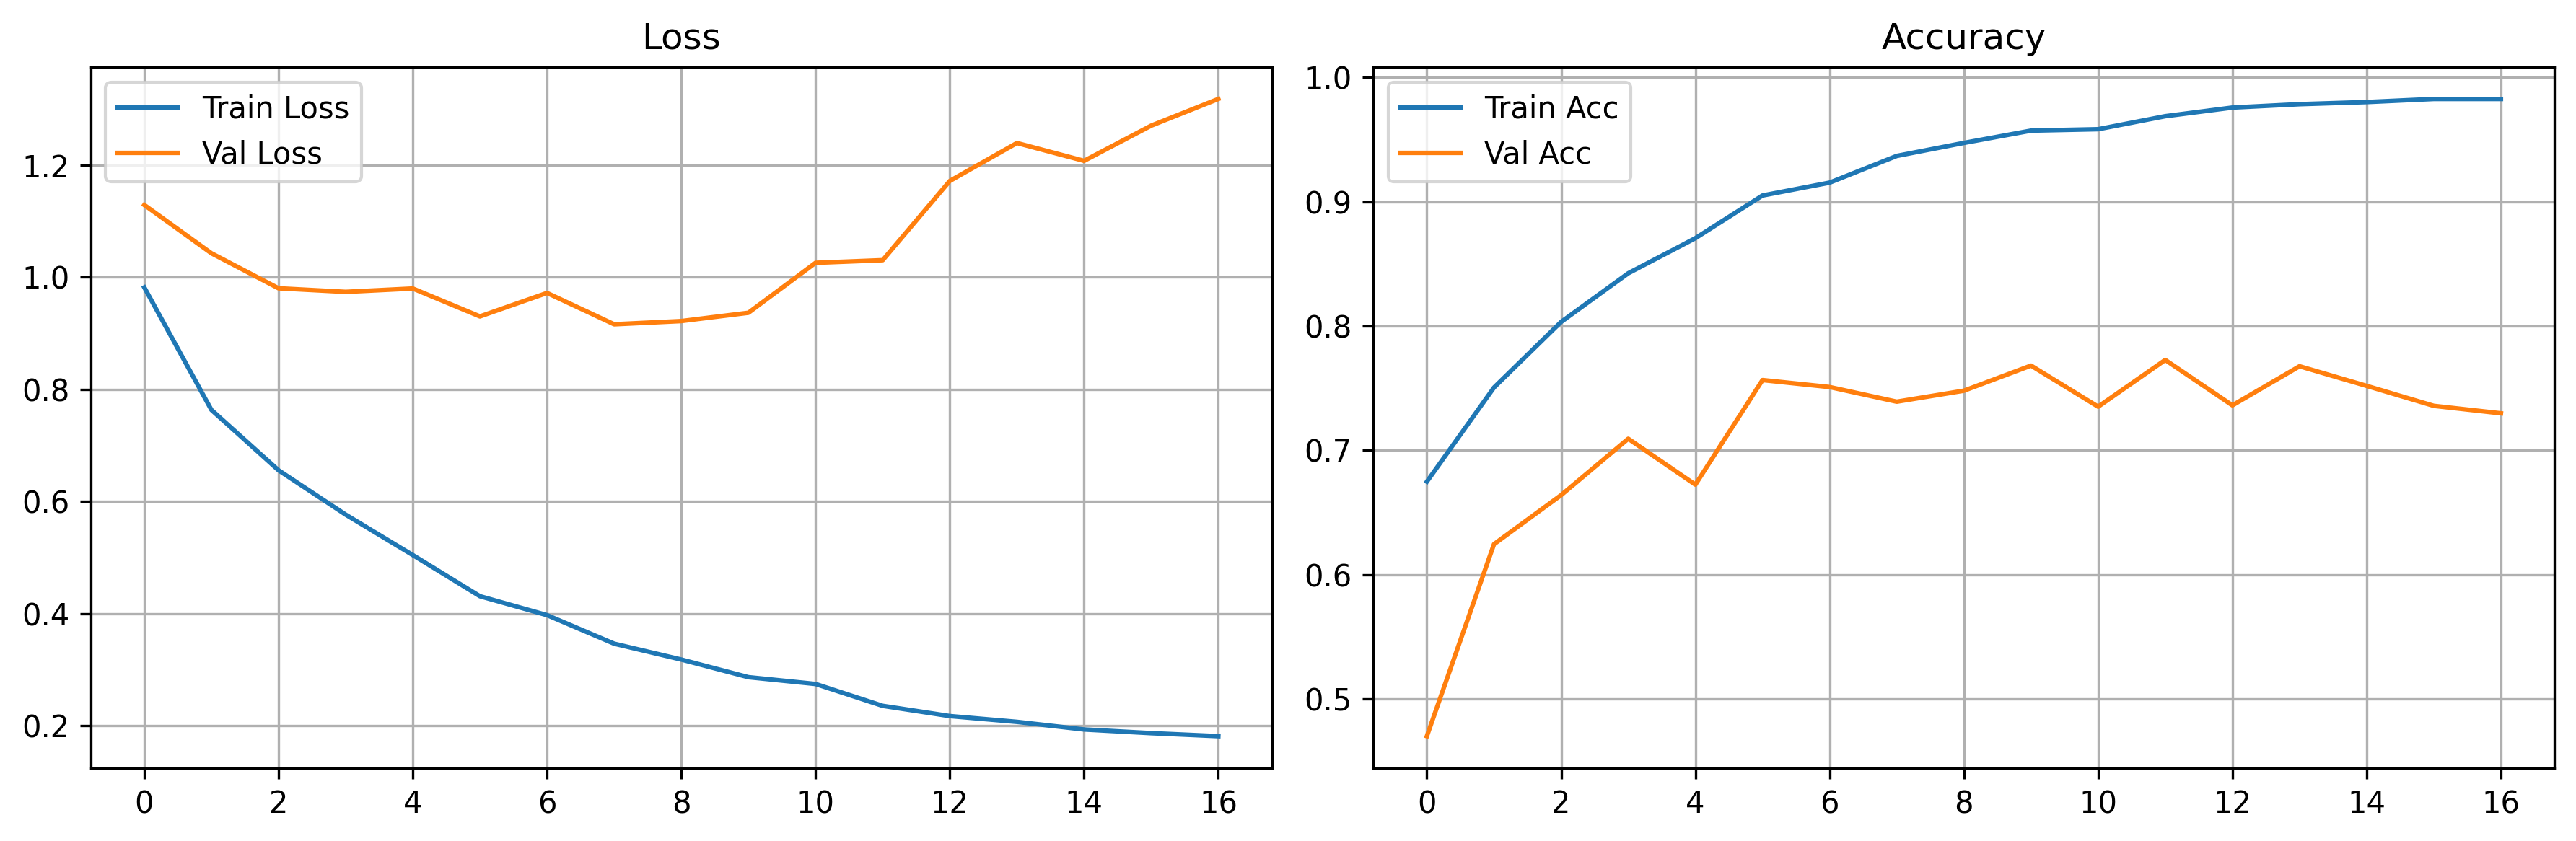
\includegraphics[width=1\textwidth]{imaxes/07_il/il_training_history.png}
  }
  \caption[Curvas de entrenamiento de los extractores visuales]{Evolución de la
  precisión y la pérdida (entrenamiento y validación) del modelo \gls{gru} de doble
  cabeza. La precisión de validación alcanza el \qty{77.3}{\percent}; el \textit{early stopping}
  detiene el entrenamiento al estancarse la mejora.}
  \label{fig:il-training}
\end{figure}


Además, las redes empleadas son considerablemente pequeñas,
como muestra la Tabla~\ref{tab:il-extractores-inferencia}
(página~\pageref{tab:il-extractores-inferencia}): la \gls{convlstm}
es la más ligera (\num{0.38}\,M de parámetros), pero queda \num{2.6} puntos por debajo de la
\gls{gru}. El \gls{vit} es el más pesado (\num{22.2}\,M, de los cuales solo quedan
\num{0.63}\,M entrenables) tras congelar las capas y, sin embargo, es el peor en
precisión. La \gls{gru} ofrece el mejor compromiso entre coste y precisión: con
\num{3.75}\,M de parámetros y sin preentrenamiento, alcanza la
mayor precisión. Esto la convierte en el modelo ganador de la iteración.

\begin{table}[htbp]
  \centering
  \resizebox{\textwidth}{!}{
  \small
  \rowcolors{2}{white}{udcgray!25}
  \begin{tabular}{l|c|c|c} 
  \rowcolor{udcpink!25}
  \textbf{Extractor} & \textbf{Parámetros} & \textbf{Preentrenamiento} & \textbf{Acc. val. (\%)} \\\hline
  \gls{gru} & \num{3.75}\,M            & No            & \textbf{\num{77.3}} \\
  \gls{convlstm}      & \num{0.38}\,M            & No            & \num{74.7} \\
  \gls{vit}    & \num{22.2}\,M \scriptsize(\num{0.63}\,M entrenables) & Sí (\textit{ImageNet}) & \num{73.2} \\
  \end{tabular}
  }
  \caption[Comparación de extractores visuales]{Comparación de tamaño de los tres
  extractores. El \gls{vit} mantiene su \gls{backbone} congelado y solo entrena la cabeza de clasificación, 
  mientras que la \gls{gru} y la \gls{convlstm} se entrenan desde cero.}
  \label{tab:il-extractores-inferencia}
\end{table}

Observando la matriz de confusión (Figura~\ref{fig:il-confusion}, página~\pageref{fig:il-confusion}) se puede apreciar de dónde provienen los errores del modelo. Las acciones \textit{attack} y \textit{move\_forward\_sprint} son las que más seguridad tienen, con un \qty{77.0}{\percent} y un \qty{91.0}{\percent} respectivamente. El principal problema
se encuentra en la acción de \textit{move\_forward\_jump}. Esto se debe a que, para un mismo \textit{frame} y estado, las acciones \textit{move\_forward\_jump} y \textit{move\_forward\_sprint} son muy similares.
Presentan diferencias sutiles, lo que provoca que el modelo no sea capaz de capturar su distinción.

\begin{figure}[htbp]
  \centering
  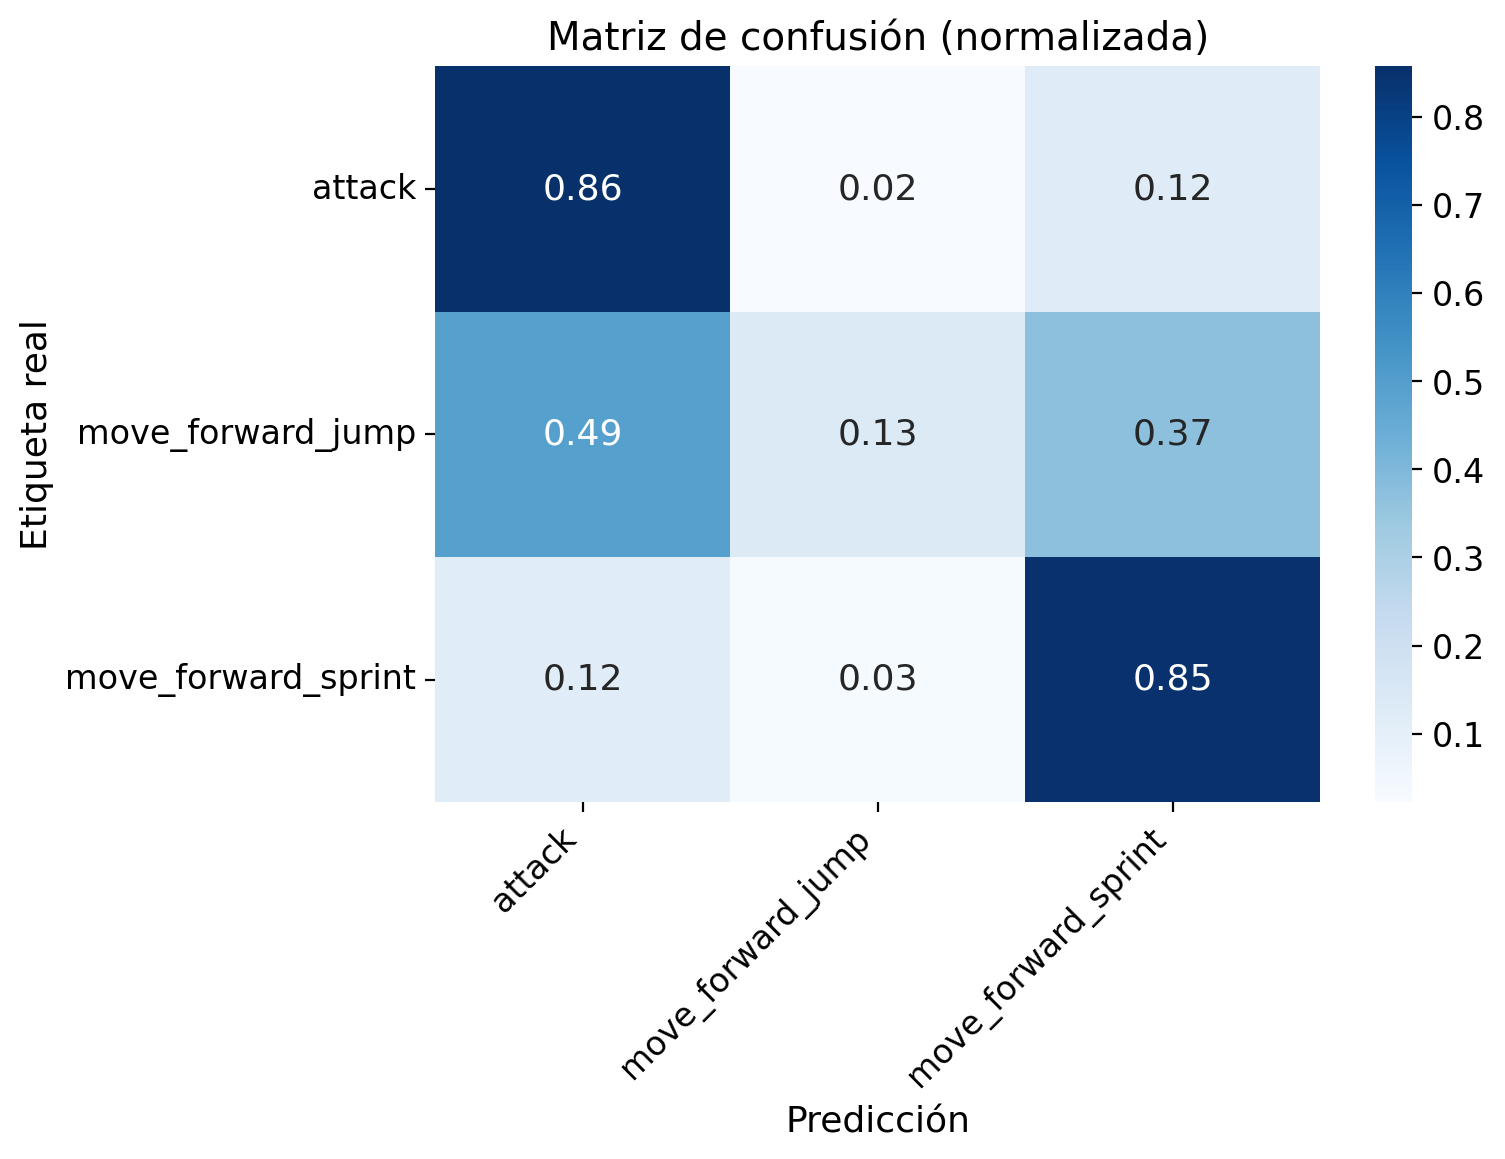
\includegraphics[width=0.7\textwidth]{imaxes/07_il/il_confusion_matrix.png}
  \caption[Matriz de confusión del agente de imitación]{Matriz de confusión sobre el
  conjunto de validación. Los errores se concentran entre las dos acciones de avance;
  la acción dominante \textit{attack} se clasifica con alta fiabilidad.}
  \label{fig:il-confusion}
\end{figure}

En las imágenes del visor (véase el Apéndice~\ref{apx:frame}), el agente simbólico podría realizar ambas acciones de movimiento:
tanto \textit{move\_forward\_sprint} como \textit{move\_forward\_jump} para llegar al mismo resultado. 
Cabe mencionar que la división de estas dos acciones es deliberada: si solo usásemos las acciones de \textit{jump} y
\textit{move\_forward\_sprint}, el agente sería incapaz de sobrepasar bloques, ya que la acción de \textit{jump}
no realiza movimiento horizontal, solo vertical.
Lo más importante es que, si reducimos las acciones a atacar y moverse, observamos que el agente sí que aprende los comportamientos de
acercarse al tronco y atacarlo (Figura~\ref{fig:il_matriz_binaria}, página~\pageref{fig:il_matriz_binaria}). La confusión que podría generarse en este escenario binario
viene dada por una razón similar: las acciones de movimiento y de ataque tienen imágenes bastante similares, diferenciándose
principalmente por la distancia al tronco y la posición de la cámara.

\begin{figure}[htbp]
  \centering
  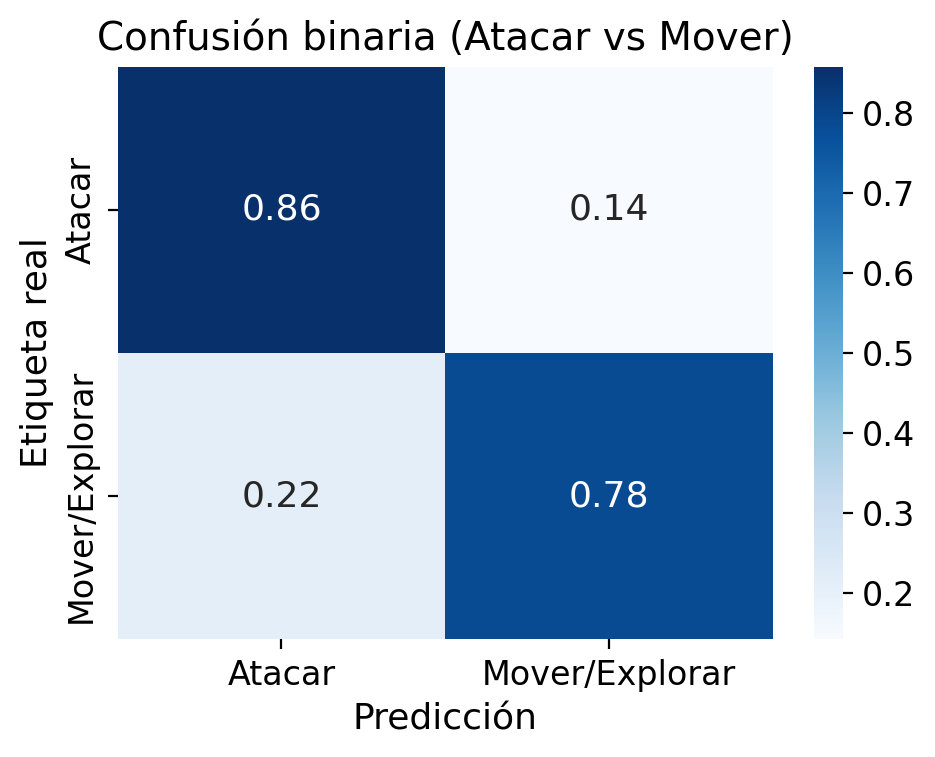
\includegraphics[width=0.5\textwidth]{imaxes/07_il/il_matriz_binaria.png}
  \caption[Matriz de confusión binaria (atacar vs movimiento)]{Matriz de confusión sobre
  el conjunto de validación colapsando las dos acciones de avance
  (\textit{move\_forward\_sprint} y \textit{move\_forward\_jump}) en una única clase
  \textbf{Mover/Explorar} frente a \textbf{Atacar}. Al eliminar la ambigüedad entre las
  dos acciones de avance, la precisión sube al \qty{83.0}{\percent} (frente al \qty{77.3}{\percent} de las
  tres clases): el agente distingue con fiabilidad cuándo acercarse al tronco
  (\qty{78}{\percent}) de cuándo talarlo (\qty{86}{\percent}).}
  \label{fig:il_matriz_binaria}
\end{figure}

\section{Servidor de inferencia}
Siguiendo la arquitectura de tres capas del Capítulo~\ref{chap:arquitectura}, el
modelo entrenado (\textit{Python}) y el control del agente (\textit{Node.js}) se comunican
por \acrshort{http}: un servidor de inferencia expone el \gls{endpoint} \textit{POST /predict},
que recibe la imagen del visor y el estado del agente y responde con la acción predicha, su
confianza y el desplazamiento de cámara desnormalizado (en radianes).

Sobre esta comunicación, el \textit{ILAgent} (capa de agentes) ejecuta un bucle
\textit{percepción} $\rightarrow$ \textit{decisión} $\rightarrow$ \textit{acción}
(Figura~\ref{fig:il-loop}, página~\pageref{fig:il-loop}): captura el
\textit{prismarine-viewer} con \textit{Puppeteer}, lo envía al servidor junto con el estado
actual y ejecuta en \textit{Mineflayer} la acción que recibe.


\begin{figure}[htbp]
  \centering
  \begin{tikzpicture}[
    font=\footnotesize, >=Latex, node distance=6mm,
    proc/.style ={draw, rounded corners, align=center, minimum width=32mm, minimum height=11mm},
    py/.style   ={proc, fill=udcpink!8},
    js/.style   ={proc, fill=udcgray!8},
    lbl/.style  ={font=\scriptsize, align=center, inner sep=2pt, fill=white},
    sw/.style   ={draw, rounded corners=1pt, minimum width=4mm, minimum height=3mm},
  ]
    % Columna 1 - izq
    \node[js] (cap)   {Captura del visor\\\scriptsize \textit{Puppeteer}};
    \node[js] (state) [below=6mm of cap] {Estado del agente};

    \path (cap.east) -- (state.east) coordinate[midway] (mid_east);

    % Columna 2 - der
    \node[py] (srv)   [right=16mm of mid_east] {Servidor de inferencia\\\scriptsize \textit{POST /predict}};
    \node[py] (model) [below=10mm of srv] {Modelo doble cabeza\\\scriptsize (acción $+\;\Delta$cámara)};
    \node[js] (post)  [below=10mm of model] {Post-proceso\\\scriptsize umbral $\cdot$ zona muerta\\\scriptsize \textit{pitch decay}};

    % Vuelta a Columna 1 
    \node[js] (exec)  at (cap |- post) {Ejecutar acción\\\scriptsize \textit{Mineflayer}};

    % Conexiones de ida
    \draw[->, rounded corners=2pt] (cap.east) -- ++(8mm,0) |- ($(srv.west)+(0,2mm)$);
    \draw[->, rounded corners=2pt] (state.east) -- ++(8mm,0) |- ($(srv.west)+(0,-2mm)$);
    \draw[->] (srv.south) -- (model.north);
    \draw[->] (model.south) -- node[lbl]{predicción} (post.north);
    \draw[->] (post.west) -- (exec.east);

    % Bucle 
    \coordinate (loop_turn) at ($(exec.west) + (-12mm, 0)$);
    \draw[->, thick, rounded corners=4pt] (exec.west) -- (loop_turn) |- (cap.west);
    \draw[->, thick] (loop_turn |- state.west) -- (state.west); % Ramificación al estado

    % Leyenda 
    \node[sw, fill=udcgray!8] (ljs) at ($(exec.south west)+(2mm,-12mm)$) {};
    \node[lbl, right=1mm of ljs, anchor=west, fill=none] {\textit{Node.js} (capa de agentes)};
    \node[sw, fill=udcpink!8] (lpy) [right=34mm of ljs] {};
    \node[lbl, right=1mm of lpy, anchor=west, fill=none] {\textit{Python} (capa de decisión)};
  \end{tikzpicture}
  \caption[Bucle de inferencia del agente de imitación]{Bucle
  \textit{percepción\,$\rightarrow$\,decisión\,$\rightarrow$\,acción} del
  \textit{ILAgent}. La captura del visor y el vector de estado (\textit{Node.js}) se envían
  al servidor de inferencia (\textit{Python}), que devuelve la acción discreta y el
  desplazamiento de cámara; la predicción se post-procesa (umbral de confianza, zona
  muerta de cámara y decaimiento de \textit{pitch}) y se ejecuta en \textit{Mineflayer},
  cerrando el bucle en tiempo real.}
  \label{fig:il-loop}
\end{figure}

Se aplican tres matices a la evaluación para adaptar la política a la ejecución en tiempo real:
\begin{itemize}
  \item \textbf{Umbral de confianza}: solo se cambia de acción si la confianza de la
  nueva supera un umbral (\num{0.7}); en caso contrario se mantiene la acción anterior.
  Esto reduce la ambigüedad entre estados similares, produciendo un comportamiento
  más estable.
  \item \textbf{Zona muerta de cámara}: los desplazamientos de cámara por debajo de
  $\sim\qty{0.01}{\radian}$ se ignoran por considerarse ruido.
  \item \textbf{Decaimiento del \textit{pitch}}: tras aplicar el delta, el \textit{pitch}
  se reduce para contrarrestar la acumulación de pequeños errores
  que, sin corrección, provocarían que el agente apuntara la cámara al suelo o al cielo.
\end{itemize}

Además, la acción discreta \textit{attack} se ejecuta como
la primitiva de minar del \gls{htn} (una vez comenzada se realiza hasta romper el bloque), 
garantizando que la acción de atacar complete la tala del bloque, igual que lo haría el experto.

\section{Resultados de la iteración}
El agente de imitación se evalúa en el mismo entorno y
bajo la misma métrica común que el resto de técnicas (recoger al menos $k$ troncos, con $k=\num{5}$).
Esto permite comparar al aprendiz con su tutor en igualdad de condiciones. En la Figura~\ref{fig:il-action-dist} 
(página~\pageref{fig:il-action-dist}) se observa la distribución de acciones del agente de imitación.

\begin{figure}[htbp]
  \centering
  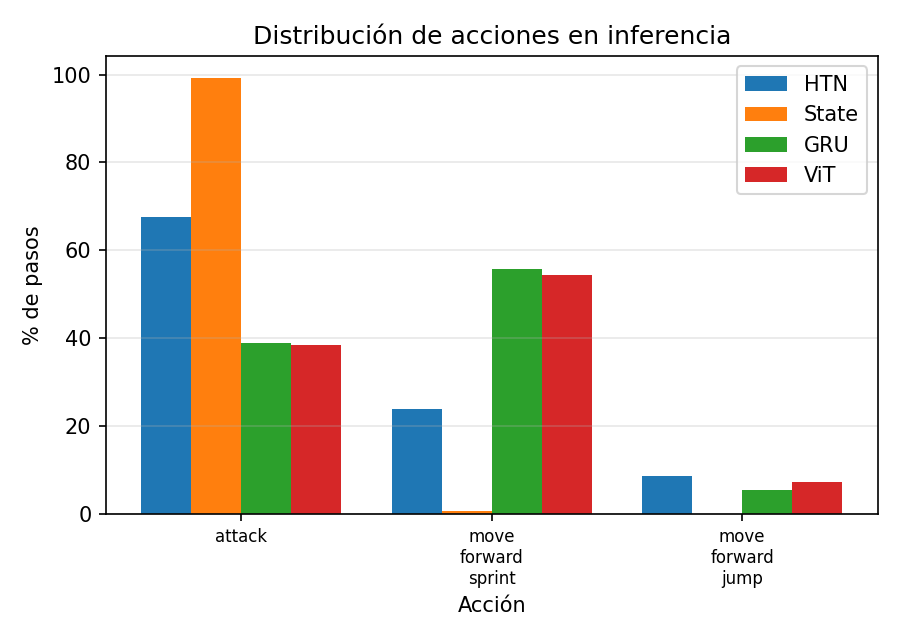
\includegraphics[width=0.8\textwidth]{imaxes/07_il/il_action_dist.png}
  \caption[Distribución de acciones del agente de imitación por técnica]{Distribución de acciones del
  agente de imitación por técnica. La \gls{gru} y la \gls{vit} presentan una distribución de acciones
  más similar a la del experto (\gls{htn}), mientras que la \gls{convlstm} y la variante solo-estado apenas se mueven 
  y atacan en casi todos los \textit{frames}.}
  \label{fig:il-action-dist}
\end{figure}

En ella podemos apreciar que las dos arquitecturas con una distribución de acciones más similar a la del
experto son la \gls{gru} y la \gls{vit}, con distribuciones similares entre sí. Las otras dos aproximaciones,
la \gls{convlstm} y la variante solo-estado, presentan una distribución de acciones muy característica:
ambas realizan la acción de atacar en casi todos los \textit{frames} y apenas se mueven. Esto indica, como
se menciona en la Sección~\ref{sec:solo-estado} (página~\pageref{sec:solo-estado}), que la información visual obtenida del extractor es
la que permite al agente aprender a moverse y atacar. Esto queda confirmado al ver el rendimiento
de la \gls{convlstm} en la Tabla~\ref{tab:il-eval} (página~\pageref{tab:il-eval}), ya que su extractor visual
es una \gls{cnn} simple, obteniendo un éxito inferior
incluso al de la variante solo-estado, que no tiene información visual. Esto indica que la \gls{cnn} no es
capaz de extraer correctamente la información de la imagen. E incluso puede llegar a reducir el funcionamiento del modelo.

\begin{table}[htbp]
  \centering
  \small
  \resizebox{\textwidth}{!}{
  \rowcolors{3}{white}{udcgray!25}
  \resizebox{\textwidth}{!}{
  \begin{tabular}{l|r|r|rrr|rrr}
  \rowcolor{udcpink!25}
   & & & \multicolumn{3}{c|}{\textbf{Troncos}} & \multicolumn{3}{c}{\textbf{Tiempo (s)}} \\
  \rowcolor{udcpink!25}
  \textbf{Técnica} & \textbf{Eps.} & \textbf{Éxito (\%)} & $\boldsymbol{\mu}$ & \textbf{$\tilde{x}$} & $\boldsymbol{\sigma}$ & $\boldsymbol{\mu}$ & \textbf{$\tilde{x}$} & $\boldsymbol{\sigma}$ \\\hline
  HTN & \num{50} & \num{100.0} & \num{6.00} & \num{6.00} & \num{0.00} & \num{26.7} & \num{26.4} & \num{1.1} \\
  IL-STATE & \num{50} & \num{4.0} & \num{0.54} & \num{0.00} & \num{1.25} & \num{195.8} & \num{202.1} & \num{34.1} \\
  IL-GRU & \num{50} & \num{52.0} & \num{3.84} & \num{5.00} & \num{1.82} & \num{156.2} & \num{203.4} & \num{67.3} \\
  IL-CONV & \num{50} & \num{0.0} & \num{0.08} & \num{0.00} & \num{0.27} & \num{203.0} & \num{202.1} & \num{3.3} \\
  IL-VIT & \num{32} & \num{37.5} & \num{3.00} & \num{3.50} & \num{1.90} & \num{169.4} & \num{208.6} & \num{67.9} \\
  \end{tabular}
  }
  }
  \caption[Evaluación de las técnicas de imitación]{Evaluación de las técnicas de imitación bajo la métrica común recoger $k=\num{5}$ troncos.
  Troncos y tiempo por episodio: media ($\mu$), mediana (\textbf{$\tilde{x}$}) y desviación típica ($\sigma$).}
  \label{tab:il-eval}
\end{table}


\subsection{Análisis de resultados}
\label{sec:il-sin-exploracion}
Durante el proceso de evaluación se encontró una limitación del modelo de imitación
que no se refleja en los resultados mencionados hasta ahora. El agente es capaz de
aprender la tarea de talar un árbol visible; es decir, cuando hay un tronco dentro del campo de
visión y al alcance, se orienta hacia él, se acerca y lo ataca correctamente.

Sin embargo, el agente \textbf{no presenta exploración}: es incapaz de buscar consistentemente
un árbol que esté lejos y acercarse a él. En escenarios donde el árbol no está en el campo de visión inicial,
el agente tiene un rendimiento considerablemente peor.

La causa de esta separación viene de las demostraciones generadas por el experto. Al 
localizar los troncos con la información de la \acrshort{api} y navegar de forma
óptima con el \gls{pathfinder}, nunca realiza la tarea de exploración ni realiza una búsqueda 
visual. En consecuencia, el \textit{dataset} no contiene
comportamiento exploratorio real: el aprendiz solo ha visto cómo talar
un árbol que tiene enfrente, pero no cómo encontrarlo mediante exploración. 
Teniendo esto en cuenta, todas las evaluaciones de las técnicas se realizan en un entorno
con árboles al alcance del campo de visión inicial.

\subsection{Alcance del agente de imitación}
La falta de exploración descrita es un síntoma de un problema más general de la imitación.
Cuando el agente aprendido se desvía de la trayectoria del experto, visita estados poco
representados en las demostraciones, donde la política no es tan precisa. Este problema se
denomina \textit{\gls{distribution-shift}}~\cite{DBLP:journals/jmlr/RossGB11}: los errores se
acumulan a lo largo del episodio porque el experto no enseñó cómo salir de las situaciones
que provoca el propio aprendiz.

Esta limitación es precisamente lo que motiva la Iteración~III, desarrollada en el Capítulo~\ref{chap:iter3}.
El aprendizaje por refuerzo permite que el agente \emph{explore} y corrija sus propios 
errores mediante la recompensa, en lugar de depender de un experto que cubra todas las posibilidades. 
Además, la política de imitación puede servir para inicializar el agente de refuerzo
mediante \gls{bc}, como se explora en el Capítulo~\ref{chap:conclusions}.
 \chapter{Iteración III - Agente de Refuerzo}
\label{chap:iter3}

\lettrine{L}{a} última iteración aborda el aprendizaje por refuerzo (\gls{rl}). A
diferencia del agente de imitación (Capítulo~\ref{chap:iter2}), que clona a un
experto heredando también sus defectos (Sección~\ref{sec:il-sin-exploracion}, página~\pageref{sec:il-sin-exploracion}),
el agente de refuerzo aprende su \gls{política}
interactuando con el entorno y corrigiendo sus propios errores a partir de una señal
de recompensa. Teóricamente esto le permite explorar y descubrir comportamientos
que el \textit{dataset} del experto no contiene.

Para abordar el aprendizaje por refuerzo se comparan tres algoritmos usados 
en la literatura: \gls{dqn}~\cite{DBLP:journals/nature/MnihKSRVBGRFOPB15},
\gls{ppo}~\cite{DBLP:journals/corr/SchulmanWDRK17} y \gls{sac}~\cite{DBLP:journals/corr/abs-1801-01290}.
Como en las iteraciones anteriores, la tarea es \textit{\gls{woodcutting}} y el entorno es el mismo, 
con la misma percepción y las mismas restricciones de acción. El objetivo es estudiar si el refuerzo,
aprendiendo su propia \gls{política}, es capaz de igualar o superar al resto de las técnicas.

\section{Motivación}
El agente \gls{htn} (Capítulo~\ref{chap:iter1}) decide a partir de la información
privilegiada de la \acrshort{api} y navega de forma óptima con el \gls{pathfinder}; el agente
de imitación (Capítulo~\ref{chap:iter2}) reproduce ese comportamiento, 
pero solo aprende a talar árboles visibles, no a encontrarlos,
debido a la navegación óptima del experto.

El aprendizaje por refuerzo pretende suplir estas limitaciones (conocimiento privilegiado
y ausencia de exploración), dejando además la posibilidad de descubrir estrategias que el \textit{dataset} del
experto no contiene, por ejemplo, evadir los obstáculos. 
Los fundamentos del refuerzo se describen en el Capítulo~\ref{chap:marco_teorico}. 
Sus mayores limitaciones son: definir una función de recompensa que codifique el 
objetivo de la tarea (Sección~\ref{sec:rl-reward}, página~\pageref{sec:rl-reward}) y el tiempo de 
exploración del entorno por parte del agente (Tabla~\ref{tab:rl-comparativa}, página~\pageref{tab:rl-comparativa}).

\section{Formulación del Problema de Refuerzo}
El bucle de aprendizaje que realiza el agente consiste en:
observar el estado del entorno, ejecutar una acción y recibir una recompensa, repitiendo
hasta una condición de \gls{terminacion} o \gls{truncamiento}. En las siguientes secciones
se describen los elementos que definen el problema de refuerzo.

\subsection{Espacio de Observación}
\label{sec:rl-obs}
La observación combina, como en el agente de imitación, una
\textbf{imagen} en primera persona y un \textbf{vector de estado}, de modo que
el agente percibe la misma información que tendría un jugador humano.

El vector de estado consta de \num{8} componentes normalizadas a $[-\num{1},\num{1}]$ mediante
cotas fijas conocidas del entorno: orientación de cámara (\textit{yaw}, \textit{pitch}),
movimiento respecto al \textit{frame} anterior ($\Delta x, \Delta z$), dos señales de percepción
obtenidas a través del \gls{fov} (\textit{tree\_visible}, \textit{tree\_distance}) y dos
señales de progreso de la tarea; \textit{log\_count}, número de troncos en el
inventario, e \textit{is\_looking\_at\_log}, si el cursor apunta a un tronco. Como en la
imitación, se excluye la posición absoluta ($x, y, z$) para no memorizar posiciones del
mundo, el movimiento útil viene de $\Delta x, \Delta z$.

En comparación con el agente de imitación, se añaden dos elementos al vector de estado:
\textit{log\_count} informa al agente del progreso en el episodio y
\textit{is\_looking\_at\_log} le ayuda a identificar cuándo está alineado con un tronco.
Ambos elementos son conocidos por un jugador, ya que puede acceder a la información de su inventario
para saber cuántos troncos lleva, y mediante la vista en primera persona puede saber si está
apuntando a un tronco o no. Estos no se utilizan en \gls{il} ya que van implícitos en la información que
otorga el experto, si realiza la acción de ataque es porque está apuntando a un tronco.

La imagen de entrada se redimensiona a $\num{128}\times\num{128}$. Dado que la red no es
recurrente (Sección~\ref{sec:rl-arch}, página~\pageref{sec:rl-arch}), la información temporal se aporta mediante
\textit{\gls{frame-stacking}}: se apilan los \num{4} últimos fotogramas en el eje de canales
($\num{4}\times\num{3} = \num{12}$ canales de entrada). Esto permite a la red inferir el movimiento,
que una sola imagen no captura. Es la técnica utilizada por las \gls{dqn}
de \textit{Atari}~\cite{DBLP:journals/nature/MnihKSRVBGRFOPB15}, el mismo mecanismo se aplica al
vector de estado.

\subsection{Espacio de Acción}
\label{sec:rl-action}
El agente dispone de siete acciones discretas: \textit{attack},
\textit{move\_forward\_sprint}, \textit{move\_forward\_jump} y cuatro acciones de cámara
(\textit{camera\_left}, \textit{camera\_right}, \textit{camera\_up},
\textit{camera\_down}). Las acciones de cámara aplican giros fijos de \qty{0.15}{\radian}
($\sim\ang{8.6}$) en \textit{yaw} y \qty{0.10}{\radian} en \textit{pitch}.

A este espacio de acciones no se añaden todas las opciones de movimiento,
ya que como se observa en la Figura~\ref{fig:dataset-clases} (página~\pageref{fig:dataset-clases}), 
el agente experto es capaz de talar un árbol sin necesidad de desplazarse 
lateralmente ni hacia atrás. Por lo que se considera que el espacio de acciones es suficiente para la tarea.

A diferencia del agente de imitación, en refuerzo la cámara se controla como una acción más.
En consecuencia, igual que ocurría en la primera versión
de cabeza única del agente de imitación (Sección~\ref{sec:il-camara-discreta}, página~\pageref{sec:il-camara-discreta}),
mover la cámara y desplazarse vuelven a ser mutuamente excluyentes.
Esta decisión de diseño se toma porque el agente de refuerzo no tiene que copiar a un experto que realice
múltiples acciones en un mismo paso, sino que aprende por sí mismo cuándo conviene mirar y cuándo desplazarse.

\subsection{Función de Recompensa}
\label{sec:rl-reward}
La \gls{funcion-recompensa} es la señal numérica que indica al agente cómo de bien o mal
lo está haciendo en cada momento; es el único canal por el que el refuerzo aprende, y su
diseño determina cómo de bueno será el rendimiento del agente. Esta señal se compone de tres términos:

\begin{itemize}
  \item \textbf{Recompensa terminal}: una bonificación grande al cumplir la condición de
  éxito del episodio. En este caso romper y recoger al menos un tronco.
  \item \textbf{Recompensas intermedias} (\textit{\gls{reward-shaping}}): señales extra que
  guían la exploración hacia el objetivo (golpear un tronco, acercarse a un árbol
  visible). Sin ellas, la recompensa sería demasiado escasa y el agente apenas 
  recibiría información de cómo realizar la tarea.
  \item \textbf{Penalización por paso}: un coste pequeño en cada paso que penaliza
  comportamientos en bucle y favorece iteraciones eficientes.
\end{itemize}

En este caso, la métrica de éxito de un episodio es romper y recoger al menos \textbf{un} tronco.
A diferencia del agente simbólico, que tiene como objetivo $k$ troncos.
La retropropagación de la recompensa para talar $k$ troncos en un solo episodio podría ser demasiado escasa,
por lo que se opta por una recompensa más corta. Con esto se busca que el agente aprenda a talar un tronco, 
y que en la evaluación final (Capítulo~\ref{chap:discusion-resultados}) se pueda expandir su rendimiento en la métrica de $k$ troncos.

Los valores empleados para el diseño de la función de recompensa se recogen en la Tabla~\ref{tab:reward}
(página~\pageref{tab:reward}). El valor de acercarse a un árbol se calcula
como la diferencia de distancia al árbol más cercano entre el paso actual y el anterior.
Esta información no se considera omnisciente ya que, aunque un jugador no pueda medir la distancia exacta a un árbol, 
sí puede percibir si se acerca o se aleja de él $X$ bloques.

\begin{table}[htbp]
  \centering
  \resizebox{\textwidth}{!}{%
  \small
  \rowcolors{2}{white}{udcgray!25}
  \begin{tabular}{c|c|c}
  \rowcolor{udcpink!25}
  \textbf{Evento} & \textbf{Valor} & \textbf{Propósito} \\\hline
  Romper un tronco          & $+\num{20.0}$ & Objetivo principal \\
  Recoger un tronco         & $+\num{5.0}$  & Señal principal de progreso \\
  Golpear un árbol          & $+\num{1.0}$  & Señal auxiliar de alineación \\
  Acercarse a un árbol      & $+\num{0.1}$  & Señal de acercamiento \\
  Éxito del episodio        & $+\num{30.0}$ & Bonificación terminal \\
  Coste por paso            & $-\num{0.05}$ & Favorecer trayectorias cortas \\
  Atacar un bloque erróneo  & $-\num{1.0}$  & Penalizar romper bloques incorrectos \\
  Terminación anticipada    & $-\num{5.0}$  & Penalización por muerte \\
  \end{tabular}
  }
  \caption[Términos de la función de recompensa]{Términos de la función de recompensa. Los valores
  positivos son mucho mayores que los negativos para favorecer el aprendizaje de la tarea principal.}
  \label{tab:reward}
\end{table}

Las recompensas positivas (romper un tronco, recogerlo y el éxito del episodio) son mucho más grandes que las intermedias y las negativas.
Esto se hace para que el agente aprenda a talar y recoger troncos, y no se quede en un comportamiento de acercarse a un árbol 
o golpearlo sin romperlo.
Además, dado el grado de libertad del agente, buscamos acotar el espacio de exploración y guiarlo hacia el objetivo de la tarea
lo máximo posible, que es talar y recoger troncos. 

\subsection{Condiciones de Terminación}
\label{sec:rl-terminacion}
Un episodio puede finalizar de cuatro formas:

\begin{itemize}
  \item \textbf{Éxito}: el agente recoge al menos un tronco y lo ha roto él
  mismo en el episodio. Esta segunda condición es una salvaguardia que evita que el agente
  recoja la madera caída de un episodio previo y la obtenga sin talar, inflando artificialmente la tasa de éxito.
  La evaluación final (Capítulo~\ref{chap:discusion-resultados}) equipara el umbral ($k$ troncos) al resto de las técnicas.
  \item \textbf{Muerte}: el agente muere durante el episodio.
  \item \textbf{Colapso de recompensa}: si la recompensa acumulada cae por debajo de un
  umbral ($-\num{10}$), el episodio se corta.
  \item \textbf{\Gls{truncamiento}}: al alcanzar el horizonte máximo de pasos
  (\textit{MAX\_STEPS}=\num{100} en entrenamiento).
\end{itemize}

\section{Arquitectura de la Red}
\label{sec:rl-arch}
Los tres algoritmos comparten el mismo \textbf{extractor de características} (visual y de
estado); lo único que cambia es la cabeza específica de cada algoritmo. Así se
garantiza que las diferencias de rendimiento se deban al algoritmo de aprendizaje y no a la
capacidad de extracción de la red. La arquitectura mostrada en la Figura~\ref{fig:rl-arch} (página~\pageref{fig:rl-arch})
procesa la imagen apilada con un extractor \gls{cnn}, la fusiona con el vector de estado igual que en la imitación, 
y sobre él cada algoritmo aplica su propia cabeza.

\begin{figure}[htbp]
  \centering
  \resizebox{\textwidth}{!}{
  \begin{tikzpicture}[
    font=\footnotesize, >=Latex, node distance=6mm,
    box/.style ={draw, rounded corners, align=center, minimum height=8mm, minimum width=18mm}, 
    inp/.style ={draw, rounded corners, align=center, fill=udcgray!20, minimum height=8mm},
    ext/.style ={box, fill=blue!8},
    fus/.style ={draw, circle, inner sep=1pt, minimum size=5mm},
    tmp/.style ={box, fill=orange!12},
    headc/.style={box, fill=green!12},
    outn/.style ={align=center},
  ]
    \node[inp] (img)   {Imagen $4{\times}$RGB\\\scriptsize(\textit{\gls{frame-stacking}}, $12$ can.)};
    \node[inp] (st)    [below=8mm of img] {Estado $4{\times}8$\\\scriptsize(cámara, $\Delta$, percepción, progreso)};

    \node[ext] (extr)  [right=6mm of img]  {\gls{cnn}\\\scriptsize 3 bloques conv};
    \node[box, fill=udcgray!10] (proj) [right=6mm of st] {\textit{Linear}\\$\to d$};

    \node[fus] (sum)   at ($(extr)!0.5!(proj) + (12mm,0)$) {$+$}; 
    \node[box, fill=udcgray!10] (mlp) [right=6mm of sum] {caract.\\$d{=}256$};

    \node[headc] (ah)  [right=6mm of mlp] {Cabeza del\\algoritmo};
    \node[outn] (ao)   [right=6mm of ah] {\scriptsize DQN: $Q$\\\scriptsize PPO: \gls{política}${+}$valor\\\scriptsize SAC: \gls{política}${+}2{\times}Q$};

    \draw[->] (img)  -- (extr);
    \draw[->] (st)   -- (proj);
    \draw[->] (extr) -- (sum);
    \draw[->] (proj) -- (sum);
    \draw[->] (sum)  -- (mlp);
    \draw[->] (mlp)  -- (ah);
    \draw[->] (ah)   -- (ao);
  \end{tikzpicture}
  }
  \caption[Arquitectura de red del agente de refuerzo]{Extractor de características común
  a los tres algoritmos y cabeza específica de cada uno. La imagen apilada ($4$ \textit{frames},
  $12$ canales) pasa por un extractor \gls{cnn}; las características visuales (dim.\ $d$) se
  suman al estado proyectado, formando un vector de características común. Sobre él,
  cada algoritmo aplica su cabeza: valores~$Q$ en \gls{dqn}; actor y crítico en \gls{ppo};
  actor y dos críticos (\textit{twin~Q}) en \gls{sac}. La temporalidad se aporta por apilado
  de fotogramas, no por recurrencia.}
  \label{fig:rl-arch}
\end{figure}

Si bien la arquitectura es similar a la del agente de imitación (Sección~\ref{sec:il-arch-dual}, página~\pageref{sec:il-arch-dual}),
existen matices que impiden su transferencia directa: 

\begin{itemize}
  \item \textbf{Criterio de selección distinto}: la \gls{gru} se seleccionó por ser la que mejor
  rendimiento obtuvo en un \textit{dataset} supervisado, estático,
  pequeño y desbalanceado de demostraciones del experto. El refuerzo optimiza otro
  objetivo (valores~$Q$ o \gls{política}) sobre datos no estacionarios que el propio
  agente genera; ser el mejor en imitación no implica serlo en refuerzo.
  \item \textbf{Temporalidad}: en la imitación la dependencia
  temporal la aportaba la \gls{lstm} sobre $T=\num{4}$ frames,
  no el extractor. Aquí esa información la da el \textit{\gls{frame-stacking}} de la entrada
  (Sección~\ref{sec:rl-obs}, página~\pageref{sec:rl-obs}), usado en la \gls{dqn} de
  \textit{Atari}~\cite{DBLP:journals/nature/MnihKSRVBGRFOPB15}. La \gls{cnn} sobre frames apilados
  ya permite capturar el movimiento.
\end{itemize}

El extractor visual es una \gls{cnn} ligera de tres bloques
convolucionales (canales $\num{12}\!\to\!\num{32}\!\to\!\num{64}\!\to\!\num{128}$), cada uno con normalización y
\gls{max-pooling}, que reduce la imagen de $\num{128}\times\num{128}$ a $\num{16}\times\num{16}$; el resultado se
aplana y se proyecta a un vector de características de dimensión \num{256}.
El vector de estado se proyecta linealmente a esa misma dimensión y se fusiona por
suma con las características visuales, igual que en la imitación. Hasta
aquí, la red es idéntica en los tres algoritmos.

Sobre ese vector de características final, cada algoritmo añade su propia \textbf{cabeza} que produce su salida característica:
\begin{itemize}
  \item \gls{dqn}: una cabeza que estima los valores~$Q$ de las siete acciones.
  \item \gls{ppo}: dos cabezas, un \emph{actor} (distribución sobre las acciones) y un
  \emph{crítico} (valor del estado).
  \item \gls{sac}: una cabeza de \emph{actor} (\gls{política}) y dos críticos~$Q$ (\textit{twin Q}).
\end{itemize}

En el diseño además se incluyó el uso de 
\gls{group-norm} en lugar de \gls{batch-norm}. Los algoritmos basados en valor mantienen
dos copias de la red (red en línea y red objetivo); \gls{batch-norm} mantiene estadísticas
globales que son distintas entre las redes y pueden desincronizar sus salidas para la misma entrada. 
\gls{group-norm} no mantiene estadísticas globales y evita esa alteración~\cite{DBLP:journals/ijcv/WuH20}.


\section{Algoritmos de refuerzo}
Se comparan tres algoritmos, cada uno representativo de una familia distinta del refuerzo:
\gls{dqn}~\cite{DBLP:journals/nature/MnihKSRVBGRFOPB15} (basado en valor),
\gls{ppo}~\cite{DBLP:journals/corr/SchulmanWDRK17} (gradiente de \gls{política} \gls{on-policy})
y \gls{sac}~\cite{DBLP:journals/corr/abs-1801-01290} (actor-crítico \gls{off-policy}).

\subsection{Deep Q-Network (DQN)}
\label{sec:rl-dqn}
El \gls{dqn}~\cite{DBLP:journals/nature/MnihKSRVBGRFOPB15} aprende una función de
valor-acción $Q(s,a)$ que estima la recompensa esperada de tomar la acción $a$
en el estado $s$; la \gls{política} elige la acción de mayor valor. Es un método
\textit{\gls{off-policy}}; las transiciones se almacenan en un \gls{replay-buffer}, 
lo que permite reutilizar la experiencia varias veces. 

Se emplea la variante \textbf{\textit{Double-DQN}}~\cite{DBLP:conf/aaai/HasseltGS16}, que separa la
selección de la acción (con la red en línea) de la evaluación de su valor (con la red
objetivo) para mitigar la sobreestimación de los valores~$Q$. La exploración
sigue una estrategia $\varepsilon$-\textit{greedy} con \emph{decaimiento a lo largo del
entrenamiento}: al principio el agente actúa casi al azar y, conforme avanza, confía cada
vez más en su \gls{política}. 

\subsection{Proximal Policy Optimization (PPO)}
\label{sec:rl-ppo}
El \gls{ppo}~\cite{DBLP:journals/corr/SchulmanWDRK17} optimiza directamente la
\gls{política} mediante ascenso de gradiente, sin usar una función de valor-acción. Es un
método \textit{\gls{on-policy}}: aprende de la misma \gls{política} que genera los datos, por lo
que recolecta un conjunto de su experiencia, realiza épocas de actualización
sobre él y lo descarta. No reutiliza experiencia antigua.

Presenta un objetivo recortado (\textit{clipped objective}), que
limita cuánto puede cambiar la \gls{política} en cada actualización y evita pasos exagerados.
Sigue un esquema \textit{actor-crítico}: el \textit{actor} produce la distribución sobre
acciones y el \textit{crítico} estima el valor del estado.

\subsection{Soft Actor-Critic (SAC)}
\label{sec:rl-sac}
El \gls{sac}~\cite{DBLP:journals/corr/abs-1801-01290} es \textit{actor-crítico} como \gls{ppo} 
pero \textit{\gls{off-policy}} como \gls{dqn}, de modo que aprende una \gls{política} 
reutilizando un \gls{replay-buffer}.
Se caracteriza por utilizar \textbf{máxima entropía}: además de maximizar la
recompensa, favorece que la \gls{política} mantenga la mayor entropía posible, lo que fomenta
una mejor exploración.

Se emplea la variante discreta del algoritmo, adaptada al espacio de siete
acciones de la tarea. Mantiene dos críticos~$Q$ para reducir la
sobreestimación al igual que la \gls{dqn}, el peso de la entropía se ajusta automáticamente
durante el entrenamiento, evitando tener que fijarlo a mano.

\section{Configuración de Entrenamiento}
\label{sec:rl-config}

\subsection{Integración con el Entorno}
Como el agente de imitación, el refuerzo sigue la arquitectura de tres capas
(Capítulo~\ref{chap:arquitectura}) y captura de la imagen con \textit{Puppeteer}. La diferencia
está en el mecanismo de control: en la imitación el agente consulta a un servidor
de inferencia; en refuerzo es el
entorno \textit{\gls{gymnasium}} el que dirige el bucle y envía las acciones al \textit{bridge}
mediante \textit{/step} y \textit{/reset}, recibiendo el estado, los eventos del agente
(bloques rotos, troncos recogidos\dots) y la recompensa (Figura~\ref{fig:rl-loop}, página~\pageref{fig:rl-loop}).

Además, \textit{/world\_reset} regenera el mundo con la misma \gls{semilla} entre
episodios, algo que no ocurría en la imitación al no tener un entrenamiento directo sobre el entorno.

\begin{figure}[htbp]
  \centering
  \resizebox{0.75\textwidth}{!}{
  \begin{tikzpicture}[
    font=\footnotesize, >=Latex, node distance=6mm,
    proc/.style ={draw, rounded corners, align=center, minimum width=32mm, minimum height=11mm},
    py/.style   ={proc, fill=udcpink!8},
    js/.style   ={proc, fill=udcgray!8},
    lbl/.style  ={font=\scriptsize, align=center, inner sep=2pt, fill=white},
    sw/.style   ={draw, rounded corners=1pt, minimum width=4mm, minimum height=3mm},
  ]
    % Columna 1 (Izquierda) - Python (Decisión y Entorno)
    \node[py] (algo)   {Algoritmo RL\\\scriptsize DQN / PPO / SAC};
    \node[py] (env)    [below=12mm of algo] {Entorno \textit{Gymnasium}\\\scriptsize \textit{MinecraftRLEnv}};

    % Columna 2 (Derecha) - Node.js (Puente y Simulación)
    \node[js] (bridge) [right=16mm of env]  {\emph{Bridge} HTTP\\\scriptsize \textit{rl\_agent.js}:8766};
    \node[js] (mc)     [below=12mm of bridge] {\textit{Minecraft}\\\scriptsize \textit{Mineflayer} + visor};

    % Conexiones de ida (Descendente y hacia la derecha)
    \draw[->, rounded corners=2pt] (algo.south) -- node[lbl, right]{acción} (env.north);
    \draw[->, rounded corners=2pt] (env.east) -- node[lbl, above]{\textit{/step}} (bridge.west);
    \draw[->, rounded corners=2pt] (bridge.south) -- (mc.north);

    % Retornos (Hacia la izquierda y hacia arriba, formando el bucle característico)
    % 1. De Minecraft al Entorno (va por debajo de la col 1 y sube por el centro)
    \draw[->, thick, rounded corners=4pt] (mc.west) -| node[lbl, near start, below]{estado, eventos, captura} (env.south);
    
    % 2. Del Entorno al Algoritmo (bucle ancho por la izquierda, idéntico al de il-loop)
    \draw[->, thick, rounded corners=4pt] (env.west) -- ++(-14mm,0) |- node[lbl, pos=0.25]{obs, recompensa} (algo.west);

    % Leyenda en la parte inferior (Alineada a la izquierda y debajo de todo)
    \node[sw, fill=udcpink!8] (lpy) at ($(env.south west |- mc.south) + (0,-10mm)$) {};
    \node[lbl, right=1mm of lpy, anchor=west, fill=none] {\textit{Python} (decisión/entorno)};
    \node[sw, fill=udcgray!8] (ljs) [right=34mm of lpy] {};
    \node[lbl, right=1mm of ljs, anchor=west, fill=none] {\textit{Node.js} (agentes/simulación)};
  \end{tikzpicture}
  }
  \caption[Bucle de entrenamiento del agente de refuerzo]{Bucle de entrenamiento. El
  entorno \textit{\gls{gymnasium}} envía una acción al \textit{bridge} (\textit{/step}); 
  el agente la ejecuta en \textit{Minecraft} y devuelve: el estado, los
  eventos y la captura del visor, a partir de los cuales el entorno calcula la observación
  y la recompensa.}
  \label{fig:rl-loop}
\end{figure}

\subsection{Mundo de Entrenamiento}
El entrenamiento se realiza en un \gls{bioma} de bosque generado con una \gls{semilla}
fija, de modo que el escenario sea consistente entre episodios. Para evitar que el agente
sobreaprenda un único estado del mundo (árboles ya talados, madera en el suelo),
el mundo se regenera periódicamente cada \num{10} episodios. En la comparación de los algoritmos
de refuerzo se emplea un punto de aparición fijo distinto del de
entrenamiento, para medir la \gls{política} en condiciones no vistas.

\subsection{Hiperparámetros}
La Tabla~\ref{tab:rl-hparams} (página~\pageref{tab:rl-hparams}) resume la configuración común y la específica de cada
algoritmo. Todos comparten la misma arquitectura de red, factor de descuento
($\gamma=\num{0.99}$), tamaño de imagen ($\num{128}\times\num{128}$), \textit{\gls{frame-stacking}} ($k=\num{4}$) y
horizonte de episodio (\num{100} pasos). El valor alto de $\gamma$ se utiliza ya que la mayor
recompensa llega al final del episodio (romper y recoger el tronco), y nos interesa que esa señal
se propague hacia atrás para considerar la secuencia de acciones que la hizo posible.

\begin{table}[htbp]
  \centering
  \resizebox{\textwidth}{!}{%
  \small
  \rowcolors{2}{white}{udcgray!25}
  \begin{tabular}{c|c|c}
  \rowcolor{udcpink!25}
  \textbf{Algoritmo} & \textbf{Hiperparámetro} & \textbf{Valor} \\\hline
  \textit{Común}   & Descuento $\gamma$          & $\num{0.99}$ \\
  \textit{Común}   & Dim.\ características / oculta & \num{256} / \num{256} \\
  \textit{Común}   & Imagen / \textit{\gls{frame-stacking}} & $\num{128}\times\num{128}$ / $k=\num{4}$ \\
  \textit{Común}   & Horizonte (pasos)           & \num{100} \\
  \textit{Común}   & Tamaño de \textit{batch}    & \num{64} \\
  \gls{dqn}        & Optimizador / \textit{lr}   & \textit{Adam} / \num{e-4} \\
  \gls{dqn}        & \Gls{replay-buffer} / \emph{warmup} & \num{1e5} / \num{3000} \\
  \gls{dqn}        & Decaimiento $\varepsilon$   & \num{10000} pasos \\
  \gls{dqn}        & Actualización red objetivo  & cada \num{2500} pasos \\
  \gls{dqn}        & \emph{Reward clip} / \emph{grad clip} & \num{1.0} / \num{10.0} \\
  \gls{ppo}        & Optimizador / \textit{lr}   & \textit{Adam} / \num{3e-4} \\
  \gls{ppo}        & \emph{Rollout} / épocas / minibatch & \num{1024} / \num{4} / \num{64} \\
  \gls{ppo}        & Recorte / \gls{gae} $\lambda$ & \num{0.2} / \num{0.95} \\
  \gls{ppo}        & Coef.\ entropía / valor     & \num{0.01} / \num{0.5} \\
  \gls{sac}        & \textit{lr} (actor/crítico/$\alpha$) & \num{3e-4} \\
  \gls{sac}        & \Gls{replay-buffer} / \emph{warmup} & \num{1e5} / \num{1000} \\
  \gls{sac}        & Soft update $\tau$          & \num{0.005} \\
  \gls{sac}        & Entropía objetivo           & \qty{98}{\percent} (auto $\alpha$) \\
  \end{tabular}
  }
  \caption[Configuración de entrenamiento del agente de refuerzo]{Configuración de entrenamiento de los algoritmos de refuerzo.}
  \label{tab:rl-hparams}
\end{table}

\subsection{Selección del \textit{Checkpoint}}
\label{sec:rl-ckpt}
Durante el entrenamiento se guarda un \textit{\gls{checkpoint}} cada \num{10} episodios. Como el
aprendizaje por refuerzo puede sufrir una reducción de rendimiento por estados no beneficiosos (puntos de aparición
donde el agente no pueda encontrar árboles, exploraciones irrelevantes), el \textit{checkpoint} final no es necesariamente el mejor.
Para cada algoritmo se selecciona el \textit{checkpoint} correspondiente al \textbf{pico de la media
móvil de la tasa de éxito} (ventana de \num{20} episodios) calculada sobre las métricas de
entrenamiento, a diferencia de la \textbf{media global} que contaría estos episodios ruidosos;
la media móvil evalúa el rendimiento del modelo en un momento seleccionado. 
El mismo criterio se aplica a los tres algoritmos.

El mejor \textit{checkpoint} de cada algoritmo según este criterio es: \textit{Double-DQN} en el
episodio~\num{130}, PPO en el episodio~\num{160} y SAC en el episodio~\num{50}. El agente aleatorio,
al no entrenar, no tiene \textit{checkpoint} y se evalúa tal cual. Estas son las versiones que se
comparan a continuación y, en el Capítulo~\ref{chap:discusion-resultados}, frente al resto de
las técnicas.

\section{Resultados de la Iteración}
\label{sec:rl-resultados}
Esta sección compara los tres algoritmos y una implementación aleatoria,
que sirve de \gls{baseline}: los algoritmos que no lo superen no están aprendiendo nada
útil o precisan de más tiempo de entrenamiento. 
Las métricas utilizadas en esta sección son: las
curvas de entrenamiento con la media móvil
(Sección~\ref{sec:rl-ckpt}, página~\pageref{sec:rl-ckpt}), los resultados de evaluación en un mundo
con punto de aparición fijo y la métrica común de $k$ troncos.

\subsection{Curvas de aprendizaje y comparativa global}
Las Figuras~\ref{fig:rl-comparativa-exito} (página~\pageref{fig:rl-comparativa-exito})
y \ref{fig:rl-comparativa-recompensa} (página~\pageref{fig:rl-comparativa-recompensa}) muestran
la tasa de éxito y la recompensa por episodio (media móvil, ventana de \num{20}) de los cuatro
agentes. La línea continua marca el progreso hasta el mejor \textit{checkpoint} y la discontinua el resto del
entrenamiento. La Tabla~\ref{tab:rl-comparativa} (página~\pageref{tab:rl-comparativa}) muestra sus valores en el pico
y la Tabla~\ref{tab:eval-comparativa-rl} (página~\pageref{tab:eval-comparativa-rl}) su rendimiento en validación.

\begin{table}[htbp]
  \centering
  \small
  \resizebox{\textwidth}{!}{%
  \rowcolors{2}{white}{udcgray!25}
  \begin{tabular}{c|c|c|c|c}
  \rowcolor{udcpink!25}
  \textbf{Algoritmo} & \textbf{Episodios} & \textbf{Éxito (\%)} & \textbf{Recompensa} & \textbf{Tiempo (h)} \\\hline
  \textit{RANDOM} & \num{200} & \num{35.0} & \num{18.04} & \num{2.0} \\
  DQN & \num{200} & \num{40.0} & \num{27.48} & \num{3.7} \\
  PPO & \num{200} & \num{65.0} & \num{32.75} & \num{2.2} \\
  SAC & \num{200} & \num{40.0} & \num{23.14} & \num{3.4} \\
  \end{tabular}
  }
  \caption[Comparativa de algoritmos de refuerzo en entrenamiento]{Comparativa de algoritmos de refuerzo durante el entrenamiento. 
  El éxito y la recompensa se miden en el pico de la media móvil (ventana de \num{20} episodios), 
  es decir, en el \textit{checkpoint} seleccionado para cada algoritmo.}
  \label{tab:rl-comparativa}
\end{table}

\begin{table}[htbp]
  \centering
  \small
  \resizebox{\textwidth}{!}{%
  \rowcolors{3}{white}{udcgray!25}
  \begin{tabular}{c|c|c|ccc|ccc}
  \rowcolor{udcpink!25}
  & & & \multicolumn{3}{c|}{\textbf{Troncos}} & \multicolumn{3}{c}{\textbf{Tiempo (s)}} \\
  \rowcolor{udcpink!25}
  \textbf{Técnica} & \textbf{Eps.} & \textbf{Éxito (\%)} & $\boldsymbol{\mu}$ & \textbf{$\tilde{x}$} & $\boldsymbol{\sigma}$ & $\boldsymbol{\mu}$ & \textbf{$\tilde{x}$} & $\boldsymbol{\sigma}$ \\\hline
  HTN & \num{50} & \num{100.0} & \num{6.00} & \num{6.00} & \num{0.00} & \num{26.7} & \num{26.4} & \num{1.1} \\
  \textit{RANDOM} & \num{50} & \num{6.0} & \num{1.50} & \num{1.00} & \num{1.52} & \num{97.6} & \num{111.1} & \num{40.3} \\
  DQN & \num{50} & \num{2.0} & \num{1.10} & \num{0.00} & \num{1.40} & \num{117.6} & \num{121.5} & \num{28.8} \\
  PPO & \num{50} & \num{12.0} & \num{2.14} & \num{2.00} & \num{1.64} & \num{114.6} & \num{124.5} & \num{43.3} \\
  SAC & \num{50} & \num{4.0} & \num{1.62} & \num{1.00} & \num{1.41} & \num{110.6} & \num{114.3} & \num{31.3} \\
  \end{tabular}%
  }
  \caption[Evaluación de las técnicas de refuerzo]{Evaluación de las técnicas de refuerzo bajo la métrica común recoger $k=\num{5}$ troncos. Troncos y tiempo por episodio: media ($\mu$), mediana (\textbf{$\tilde{x}$}), y desviación típica ($\sigma$).}
  \label{tab:eval-comparativa-rl}
\end{table}


\begin{figure}[htbp]
  \centering
  \resizebox{\textwidth}{!}{%
  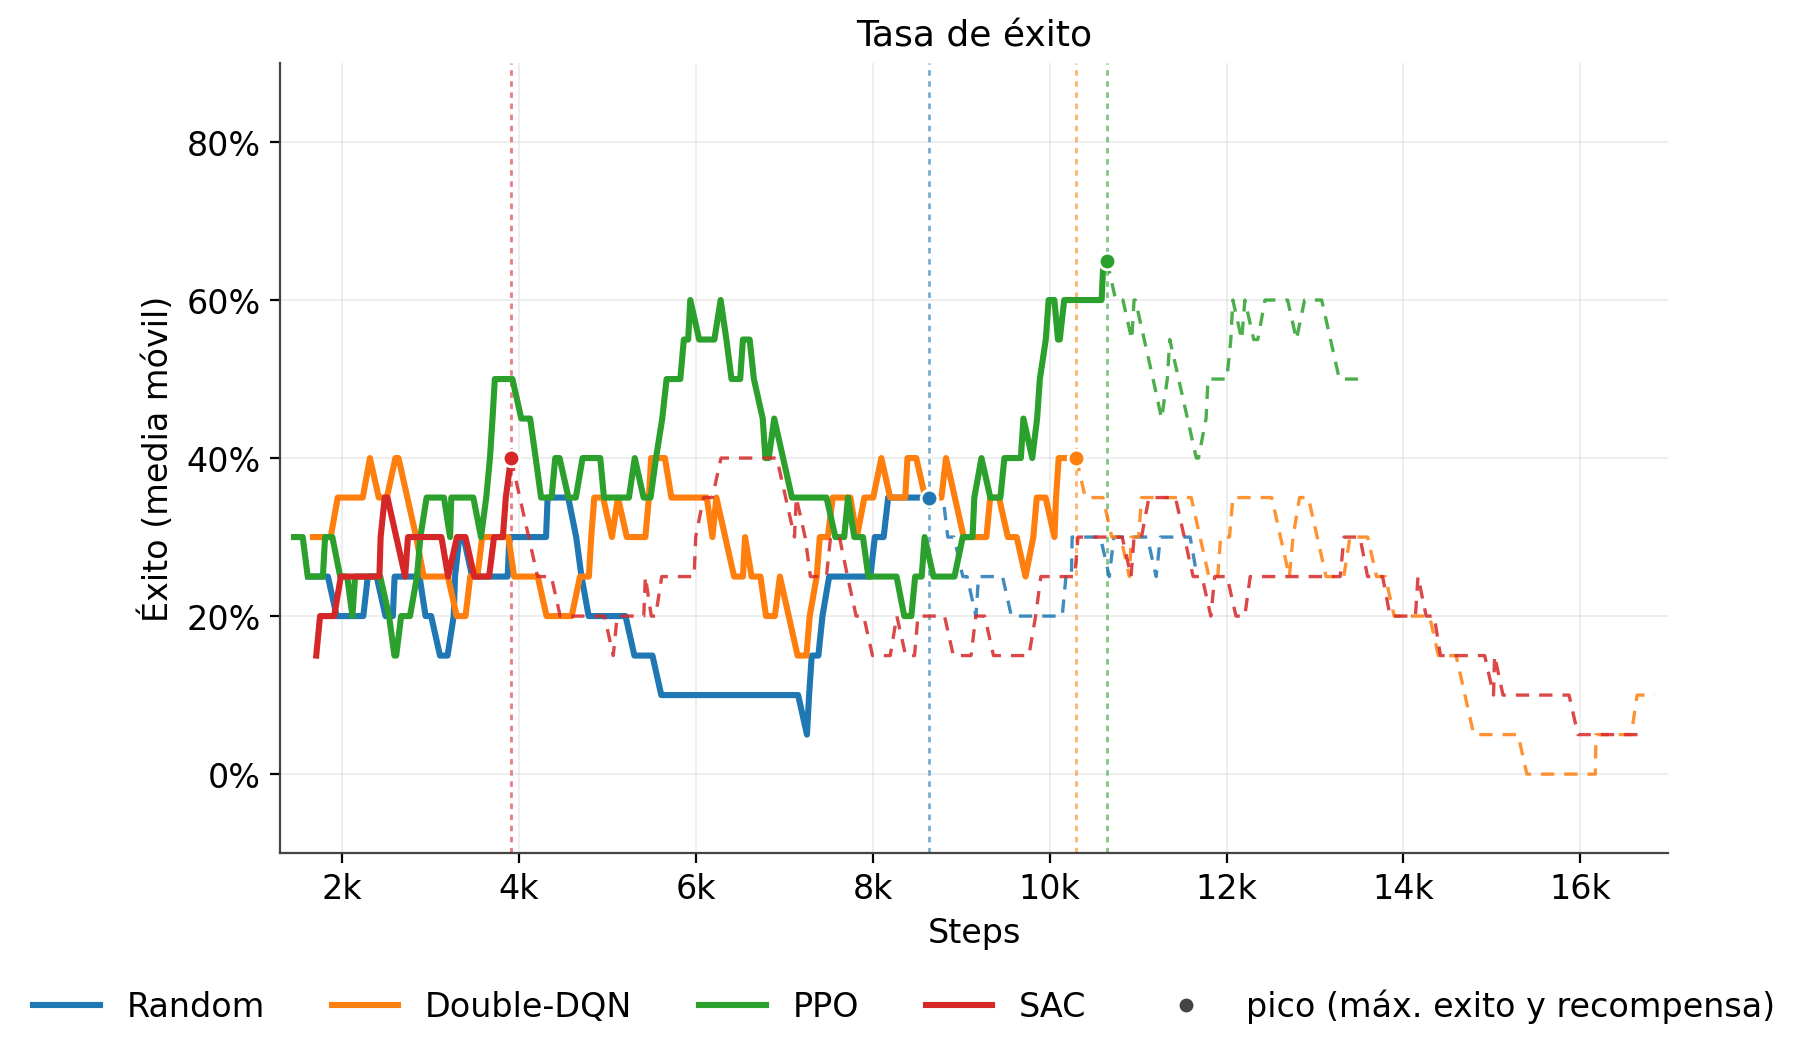
\includegraphics[width=1\textwidth]{imaxes/08_rl/comparativa_rl_exito.png}
  }
  \caption[Tasa de éxito (media móvil, ventana 20)]{Tasa de éxito durante el
  entrenamiento (media móvil, ventana de \num{20} episodios). PPO obtiene el mejor rendimiento,
  seguido de DQN y SAC; los tres superan al agente aleatorio. La línea continua llega hasta
  el mejor \textit{checkpoint} y la discontinua hasta el final del entrenamiento.}
  \label{fig:rl-comparativa-exito}
\end{figure}

\begin{figure}[htbp]
  \centering
  \resizebox{\textwidth}{!}{%
  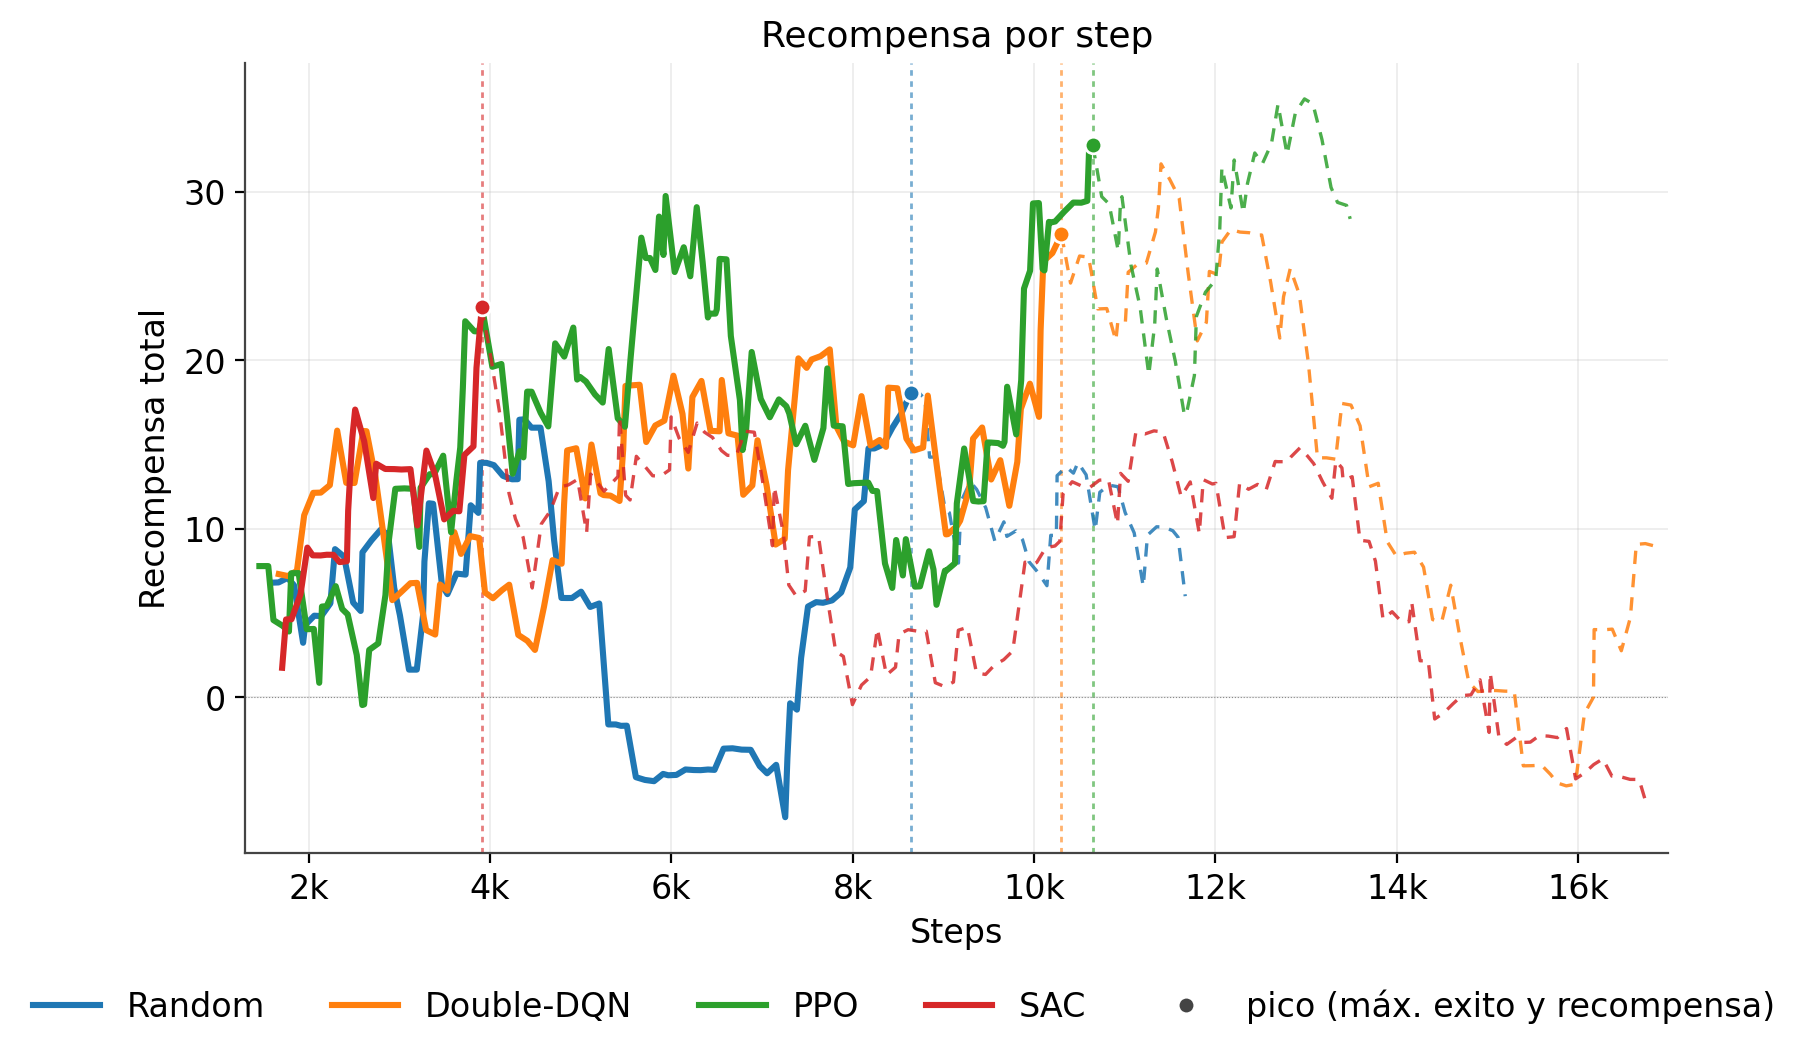
\includegraphics[width=1\textwidth]{imaxes/08_rl/comparativa_rl_recompensa.png}
  }
  \caption[Recompensa por episodio (media móvil, ventana 20)]{Recompensa total por
  episodio durante el entrenamiento (media móvil, ventana de \num{20} episodios). El orden
  coincide con el de la tasa de éxito. La caída final de SAC por debajo de cero es
  coherente con su inestabilidad (Figura~\ref{fig:rl-estabilidad}, página~\pageref{fig:rl-estabilidad}).}
  \label{fig:rl-comparativa-recompensa}
\end{figure}

El algoritmo con mejor rendimiento es \gls{ppo}, alcanza la mayor tasa de éxito en el
pico (\qty{65}{\percent}) y la mayor recompensa (\num{32.75}), y su curva mantiene una tendencia
ascendente, lo que sugiere que con más episodios
podría seguir mejorando. \gls{dqn} y \gls{sac} quedan por detrás, ambos rondando el \qty{40}{\percent}
de éxito en el pico; su tendencia indica un deterioro, aunque para confirmarlo sería necesario
un mayor número de episodios para observar realmente si se estabilizan o siguen cayendo.
Aun así, los tres algoritmos superan a la \gls{baseline} aleatoria (\qty{35}{\percent}, \num{18.04} de
recompensa), lo que confirma que sí hay aprendizaje.

Conviene matizar que las caídas observadas no son principalmente un
problema de exploración, sino la dificultad de la tarea combinada con el
diseño del mundo ya que el punto de aparición se mantiene fijo durante \num{10} episodios
(Sección~\ref{sec:rl-config}, página~\pageref{sec:rl-config}). Si en ese punto no hay árboles cercanos, el agente cae en
un agujero o queda atrapado, encadena varios episodios sin éxito que hunden la media móvil,
independientemente de si el agente aprendió a evitar esas situaciones o no. 
Esto explica por qué la curva final (línea discontinua) no se estabiliza o continúa descendiendo, y refuerza 
la elección del pico de la media móvil frente al \textit{\gls{checkpoint}} final.


\subsection{Estabilidad del entrenamiento}
\label{sec:rl-estabilidad}
La diferencia entre PPO y los otros dos algoritmos no solo está en la tasa de éxito, sino
en la estabilidad del proceso. La Figura~\ref{fig:rl-estabilidad} (página~\pageref{fig:rl-estabilidad}) muestra dos
señales propias de los algoritmos que pueden ayudar a explicar el deterioro de \gls{dqn} y \gls{sac}.

\begin{figure}[htbp]
  \centering
  \resizebox{\textwidth}{!}{%
  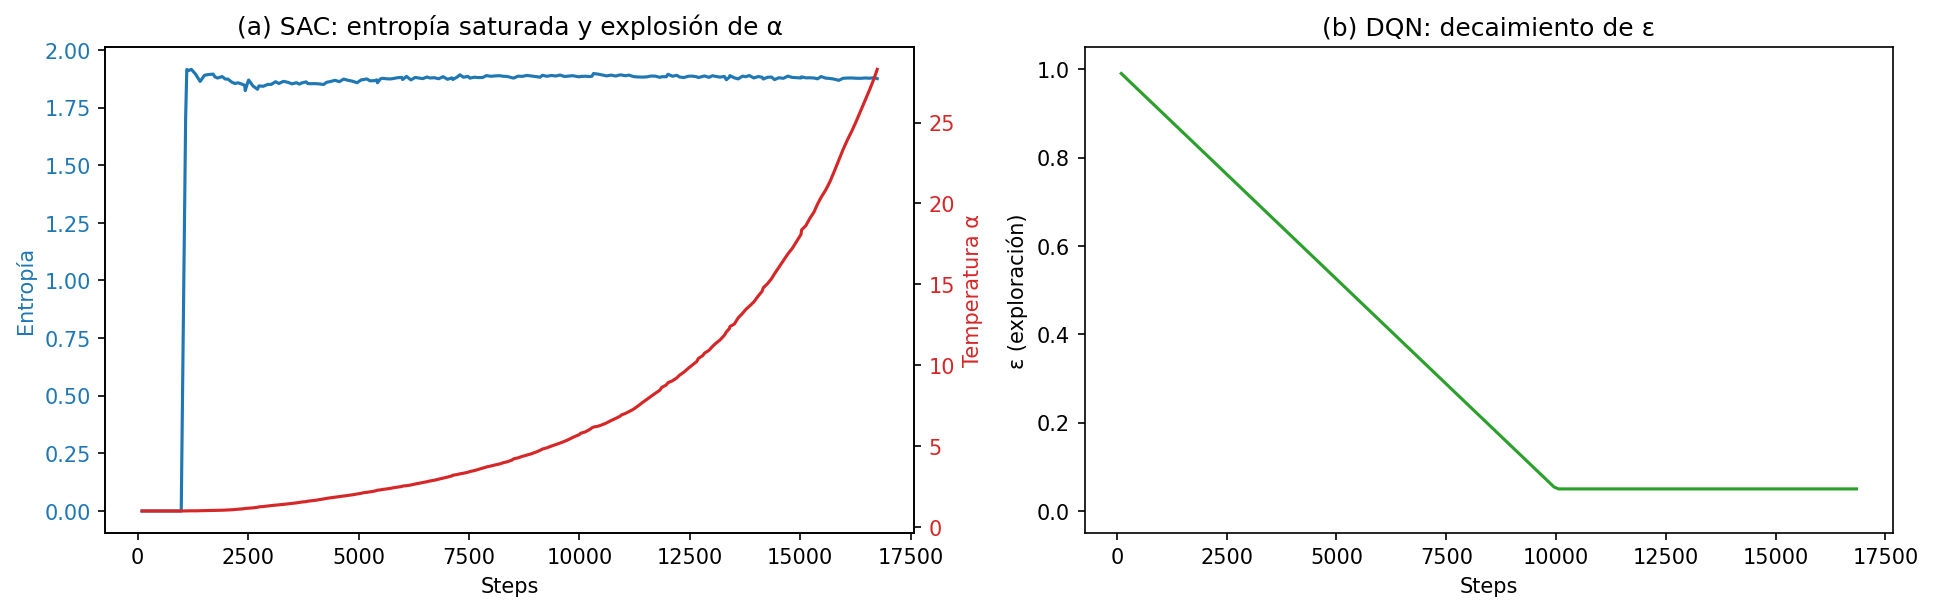
\includegraphics[width=1\textwidth]{imaxes/08_rl/estabilidad_rl.png}
  }
  \caption[Señales de estabilidad de SAC y DQN]{Señales internas del entrenamiento.
  \textbf{(a)}: en SAC, la temperatura $\alpha$ (rojo) se dispara mientras la entropía
  de la \gls{política} (azul) permanece cerca de su máximo, indicando que el término de
  entropía domina y la \gls{política} nunca se vuelve decisiva. \textbf{(b)}: en DQN, el
  decaimiento programado de $\varepsilon$ funciona correctamente. Pero la red
  podría aprovecharse de un mayor periodo de exploración.}
  \label{fig:rl-estabilidad}
\end{figure}

En \gls{sac} (a), la temperatura de entrenamiento ($\alpha$) se ajusta de forma
automática (Sección~\ref{sec:rl-sac}, página~\pageref{sec:rl-sac}). 
En la práctica $\alpha$ no se estabiliza, sino que
crece sin control (de $\sim\num{1}$ a $\sim\num{28}$ al final del entrenamiento), de forma que
la entropía termina dominando a la recompensa, y el agente no llega a fijar
una \gls{política} concreta. Su entropía acaba llegando a $\approx\num{2}$ rápidamente,
indicando que la \gls{política} es casi uniforme y el agente actúa de forma aleatoria.
Esto corresponde con la caída de su recompensa por debajo de cero
(Figura~\ref{fig:rl-comparativa-recompensa}, página~\pageref{fig:rl-comparativa-recompensa}) y
su distribución de acciones (Figura~\ref{fig:rl-acciones}, página~\pageref{fig:rl-acciones}).
Se probaron distintos valores de entropía objetivo (\num{-1}, \num{-2} y \num{-3}), pero en todos 
los casos $\alpha$ continúa creciendo sin control y la \gls{política} no se vuelve decisiva.
No se descarta el rendimiento de SAC, pero su aplicabilidad requiere 
un ajuste más fino de hiperparámetros y un mayor número de episodios de entrenamiento.


En \gls{dqn} (b) la exploración la controla $\varepsilon$, que decae de forma
uniforme de \num{1.0} a \num{0.05} a lo largo de los primeros $\sim\num{10000}$ pasos. 
El mejor rendimiento obtenido por la \gls{dqn} se obtiene alrededor de los $\sim\num{10000}$ pasos.
El punto donde la red comienza su explotación es visible en la Figura~\ref{fig:rl-comparativa-exito} (página~\pageref{fig:rl-comparativa-exito}).
Con un mayor periodo de exploración, la \gls{dqn} podría haber alcanzado un mejor rendimiento 
al poder aprender mejor las variaciones del entorno.


\subsection{Distribución de acciones}
\label{sec:rl-acciones}
La Figura~\ref{fig:rl-acciones} (página~\pageref{fig:rl-acciones}) muestra la distribución de cada una de las siete
acciones durante la evaluación de los cuatro agentes.

El agente \textbf{aleatorio} reparte las acciones de forma uniforme. 
\gls{sac} es muy similar a la versión aleatoria, lo que confirma
el análisis de la sección anterior: la explosión de $\alpha$ lo deja en una \gls{política}
casi aleatoria. \gls{dqn} sí muestra una distribución de aprendizaje; gran parte de las acciones
realizadas son \textit{camera\_down}, seguido de \textit{camera\_up}. Esto corresponde con el proceso de tala
que podría realizar un jugador humano; al talar el tronco que tiene a la altura de los ojos, la red aprende a talar
los troncos adyacentes en el eje vertical. 
\gls{ppo}, en cambio, es el único que reparte el peso entre
las acciones más relevantes de la tarea: \textit{attack}, \textit{move\_forward\_sprint}
y \textit{move\_forward\_jump}, que es justo la combinación de
avanzar hacia un árbol y golpearlo que sigue el experto.

\begin{figure}[htbp]
  \centering
  \resizebox{0.9\textwidth}{!}{%
  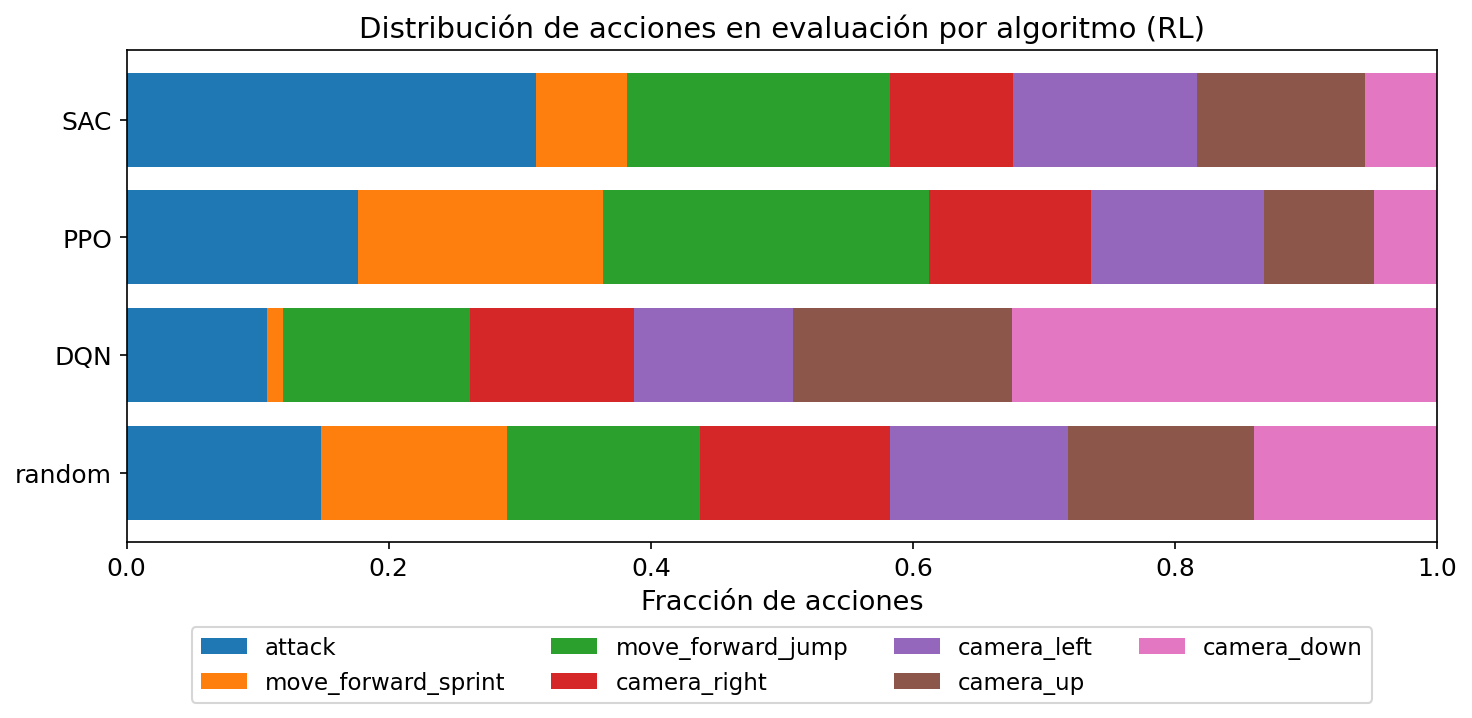
\includegraphics[width=0.8\textwidth]{imaxes/08_rl/accion_dist_rl.png}
   }
  \caption[Distribución de acciones por algoritmo de refuerzo]{Fracción de cada acción durante la
  evaluación. SAC y el agente aleatorio reparten las acciones de forma casi uniforme; DQN
  se concentra en \textit{camera\_down}; PPO favorece las acciones
  productivas de la tarea (\textit{attack} y movimiento).}
  \label{fig:rl-acciones}
\end{figure}

\begin{figure}[htbp]
  \centering
  \resizebox{0.8\textwidth}{!}{%
  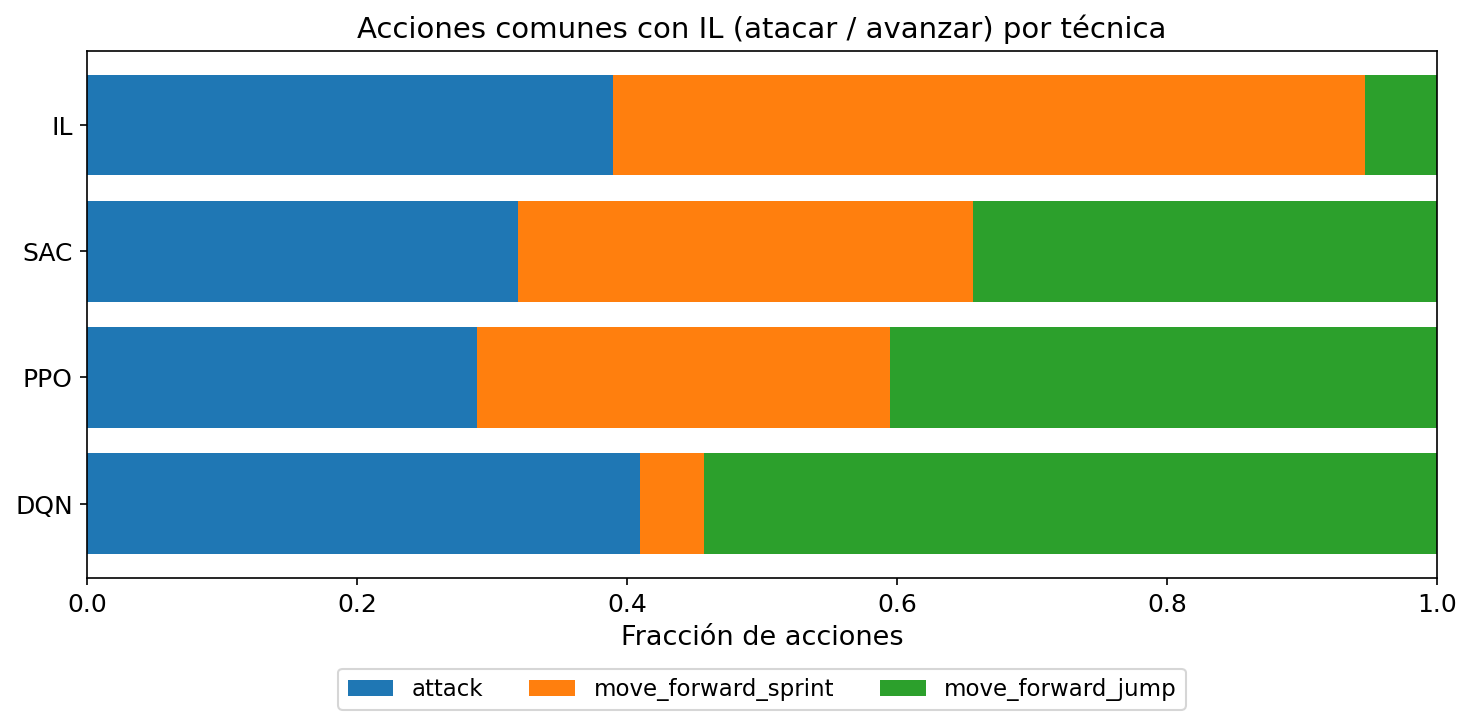
\includegraphics[width=0.8\textwidth]{imaxes/08_rl/accion_dist_comun.png}
  }
  \caption[Distribución de acciones por algoritmo de refuerzo con el mismo espacio de acciones que el agente de imitación.]{
  Fracción de cada acción durante la
  evaluación, eliminando las acciones que no están en el espacio de acciones del agente de imitación.}
  \label{fig:rl-acciones-comun}
\end{figure}

Además, la Figura~\ref{fig:rl-acciones-comun} (página~\pageref{fig:rl-acciones-comun}) 
muestra la distribución de acciones de los tres algoritmos de refuerzo, eliminando las acciones que no están en el espacio
de acciones de imitación (Sección~\ref{sec:il-arch-dual}, página~\pageref{sec:il-arch-dual}). Es decir, eliminando el componente
de la cámara, para ver si los algoritmos de refuerzo aprenden el mismo tipo de distribución que
la imitación del experto. El más cercano a la distribución es curiosamente el \textbf{DQN}, 
que aunque presenta un éxito menor al de PPO, sí aprende a moverse hacia el árbol y golpearlo.
Aunque con las acciones de movimiento intercambiadas en relación al \gls{il}, el 
\textit{move\_forward\_sprint} en \gls{dqn} tiene la misma distribución que
\textit{move\_forward\_jump} en \gls{il}, y viceversa.  

\subsection{Discusión}
El refuerzo parece ser la técnica con un mayor horizonte de desarrollo, pero en consecuencia
presenta el mayor coste computacional y temporal. La literatura (Capítulo~\ref{chap:sota}) 
muestra que el refuerzo puede aprender tareas de \textit{Minecraft} como la tala de árboles,
o la obtención de diamante~\cite{guss2019minerl}. Pero a coste de un inmenso conjunto de datos y tiempo de entrenamiento.
El número de episodios de entrenamiento utilizados en este trabajo es muy bajo en comparación con
otros trabajos. Por ejemplo, los agentes de \textit{MineRL}~\cite{guss2019minerl} emplean para la misma tarea 
de tala unos \num{1500} episodios (del orden de \num{12} millones de pasos), lo que en nuestro entorno equivaldría a unas
\num{1800} horas de cómputo (unos \num{75} días continuos) por algoritmo.

Los resultados de esta iteración muestran que el refuerzo es capaz de aprender la tarea, aunque
sin llegar a un rendimiento comparable al de la aproximación simbólica o de imitación. Pero también muestran 
que el refuerzo puede no requerir de un conjunto de datos y
tiempo de cómputo tan grande como el de \textit{MineRL}~\cite{guss2019minerl}. Con un conjunto de datos de 
\num{200} episodios (unas \num{2} horas de cómputo) es posible obtener un rendimiento aceptable
que muestre tendencias hacia un rendimiento óptimo.
 \chapter{Discusión de Resultados}
\label{chap:discusion-resultados}

\lettrine{E}{ste} capítulo realiza una comparación de todas las
técnicas implementadas a lo largo del trabajo:
\gls{htn} (Capítulo~\ref{chap:iter1}), \gls{il}
(Capítulo~\ref{chap:iter2}) y \gls{rl} (Capítulo~\ref{chap:iter3}).
Todas ellas entrenadas y evaluadas sobre la misma tarea y bajo una métrica común 
de tasa de éxito: talar $k=\num{5}$ troncos. 

Si bien en cada capítulo se analizan en profundidad los resultados de cada implementación, 
este capítulo pretende generar un análisis más general comparando todas las familias. 

\section{Metodología de Evaluación}
\label{sec:eval-metodologia}
Todas las técnicas se evalúan bajo las mismas condiciones para que la comparación sea justa.
Cada agente ejecuta \textbf{\num{50} episodios} en el mismo mundo, con un \textbf{punto de
aparición fijo} y distinto del usado en el entrenamiento, de modo que ninguna
técnica evalúe sobre un entorno que haya visto. Entre episodios el mundo se reinicia al mismo
estado con la misma \gls{semilla}, de modo que todas las técnicas se enfrentan al mismo entorno.
Cada episodio se trunca a un máximo de \num{200} pasos para contabilizar la eficiencia.
La semilla concreta no es relevante, cualquier mundo con un árbol en el campo de visión inicial es válido, ya que el objetivo es evaluar la habilidad de talar y recoger, no la búsqueda mediante exploración ciega.

La métrica de éxito es común a todos los algoritmos; un episodio se considera exitoso
si el agente \emph{rompe y obtiene al menos $k=\num{5}$ troncos}. Esta métrica se utiliza para mostrar las limitaciones 
de los algoritmos; el \gls{htn} siempre va a recoger el tronco que tala, pero el \gls{il}, al igual que en la
exploración, es posible que no recoja los troncos. Lo mismo ocurre en \gls{rl}, aunque en menor medida. Se exige recoger y no solo romper porque el fin de talar es obtener el recurso, que un agente rompa un tronco sin recogerlo no es el objetivo de la tarea.

\section{Resultados por Familia}
\label{sec:eval-familias}
Junto a la tasa de éxito se reportan métricas auxiliares por episodio: troncos recogidos 
(media ($\mu$), mediana ($\tilde{x}$) y desviación típica ($\sigma$)) y tiempo empleado.
La Tabla~\ref{tab:eval-comparativa} (página~\pageref{tab:eval-comparativa}) reúne la tasa de éxito, los troncos recogidos y el tiempo
por episodio de cada técnica. La Figura~\ref{fig:eval-exito} (página~\pageref{fig:eval-exito})
ofrece la comparación visual de la tasa de éxito por técnica.

\begin{table}[htbp]
  \centering
  \small
  \rowcolors{3}{white}{udcgray!25}
  \resizebox{\textwidth}{!}{
  \begin{tabular}{c|c|c|ccc|ccc}
  \rowcolor{udcpink!25}
   & & & \multicolumn{3}{c|}{\textbf{Troncos}} & \multicolumn{3}{c}{\textbf{Tiempo (s)}} \\
  \rowcolor{udcpink!25}
  \textbf{Técnica} & \textbf{Eps.} & \textbf{Éxito (\%)} & $\boldsymbol{\mu}$ & \textbf{$\tilde{x}$} & $\boldsymbol{\sigma}$ & $\boldsymbol{\mu}$ & \textbf{$\tilde{x}$} & $\boldsymbol{\sigma}$ \\\hline
  HTN & \num{50} & \num{100.0} & \num{6.00} & \num{6.00} & \num{0.00} & \num{26.7} & \num{26.4} & \num{1.1} \\
  RL-\textit{RANDOM} & \num{50} & \num{6.0} & \num{1.50} & \num{1.00} & \num{1.52} & \num{97.6} & \num{111.1} & \num{40.3} \\
  RL-DQN & \num{50} & \num{2.0} & \num{1.10} & \num{0.00} & \num{1.40} & \num{117.6} & \num{121.5} & \num{28.8} \\
  RL-PPO & \num{50} & \num{12.0} & \num{2.14} & \num{2.00} & \num{1.64} & \num{114.6} & \num{124.5} & \num{43.3} \\
  RL-SAC & \num{50} & \num{4.0} & \num{1.62} & \num{1.00} & \num{1.41} & \num{110.6} & \num{114.3} & \num{31.3} \\
  IL-\textit{STATE} & \num{50} & \num{4.0} & \num{0.54} & \num{0.00} & \num{1.25} & \num{195.8} & \num{202.1} & \num{34.1} \\
  IL-CONV & \num{50} & \num{0.0} & \num{0.08} & \num{0.00} & \num{0.27} & \num{203.0} & \num{202.1} & \num{3.3} \\
  IL-GRU & \num{50} & \num{52.0} & \num{3.84} & \num{5.00} & \num{1.82} & \num{156.2} & \num{203.4} & \num{67.3} \\
  IL-VIT & \num{50} & \num{46.0} & \num{3.48} & \num{4.00} & \num{2.03} & \num{156.7} & \num{206.1} & \num{70.9} \\
  \end{tabular}
  }
  \caption[Evaluación de las técnicas]{Evaluación de las técnicas bajo la métrica común recoger $k=\num{5}$ troncos.
  Troncos y tiempo por episodio: media ($\mu$), mediana (\textbf{$\tilde{x}$}), y desviación típica ($\sigma$).}
  \label{tab:eval-comparativa}
\end{table}

\begin{figure}[htbp]
  \centering
  \resizebox{\textwidth}{!}{
  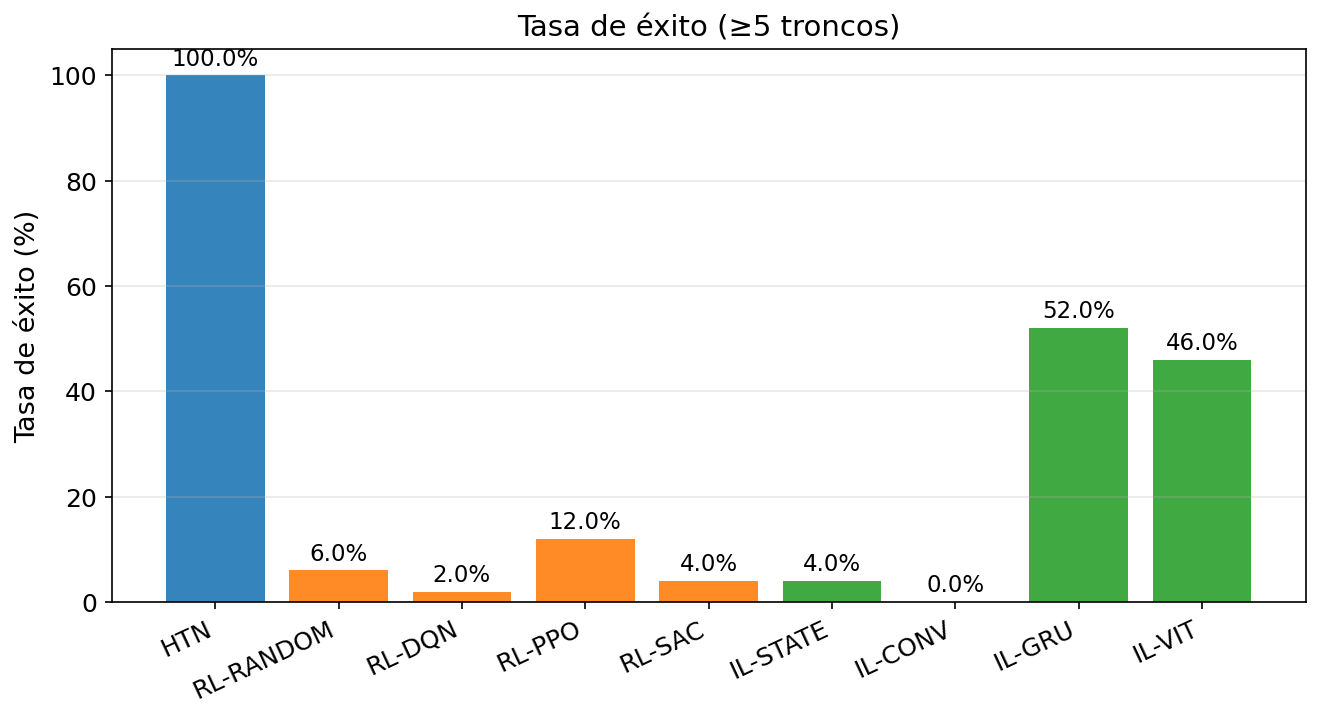
\includegraphics[width=1\textwidth]{imaxes/09_resultados/eval_exito.png}
  }
  \caption[Tasa de éxito por técnica]{Tasa de éxito en entorno bajo la métrica común
  ($\geq \num{5}$ troncos, \num{50} episodios). El \gls{htn} alcanza el objetivo el \qty{100}{\percent} de las veces; 
  entre los agentes entrenados, IL-GRU (\qty{52}{\percent}) e IL-VIT (\qty{46}{\percent}) destacan claramente
  sobre el refuerzo y el agente aleatorio.}
  \label{fig:eval-exito}
\end{figure}

\subsection{Agente Experto}
El \gls{htn} obtiene un \textbf{\qty{100}{\percent} de éxito}, recogiendo exactamente \num{6} troncos por
episodio en \qty{26.7}{\second} de media. El tronco de más sobre el objetivo ($k=\num{5}$) se debe a
que el agente tala el árbol completo antes de reevaluar la condición de parada: la primitiva
de tala rompe todo el tronco de una vez y, en el mundo de evaluación (\gls{semilla} fija), ese árbol
tiene \num{6} bloques. De ahí también su desviación típica nula.
Este resultado era esperable: el planificador opera sobre la información
de la \acrshort{api} y navega de forma óptima con el \gls{pathfinder}
(Capítulo~\ref{chap:iter1}). Su tasa de éxito y eficacia lo convierten en la cota superior 
de la tarea y el límite a alcanzar por el resto de técnicas.

\subsection{Aprendizaje por Imitación}
La \textbf{IL-GRU} es la mejor técnica de todos los agentes
entrenados, con un \textbf{\qty{52}{\percent} de éxito} y una mediana de \num{5} troncos. A diferencia del \gls{htn}, el objetivo se
comprueba una vez por paso de inferencia, de modo que entre comprobaciones el agente puede
recoger varios troncos a la vez; por eso sus episodios exitosos terminan con \num{5}, \num{6} o \num{7}
troncos (Figura~\ref{fig:eval-exito}, página~\pageref{fig:eval-exito}).
La variante \gls{vit} llega a un \qty{46}{\percent}, mientras que las
variantes más simples no consiguen un rendimiento apreciable: solo-estado se queda en el \qty{4}{\percent}
y \gls{convlstm} en el \qty{0}{\percent}. Esto confirma la importancia de la extracción de información de la
imagen en la tarea de imitación. 

Como se menciona en la Sección~\ref{sec:il-sin-exploracion} (página~\pageref{sec:il-sin-exploracion}), el agente aprende
a talar un árbol visible, pero no a encontrarlo. De ahí que falle cerca de la
mitad de los episodios, o bien porque no tiene un árbol delante o porque se pasa de largo y no lo detecta.

\subsection{Aprendizaje por Refuerzo}
El refuerzo desde cero queda muy por debajo respecto a las técnicas de imitación.
El mejor algoritmo es \textbf{PPO} con un
\textbf{\qty{12}{\percent} de éxito}, seguido del agente aleatorio (\qty{6}{\percent}), \gls{sac} (\qty{4}{\percent}) y
\gls{dqn} (\qty{2}{\percent}). El dato más importante es que \gls{dqn} y \gls{sac} no superan al
\textit{\gls{baseline}} aleatorio, indicando que no llegan a consolidar una política útil. 
Solo PPO se separa del \textit{\gls{baseline}}. Sin embargo, cabe mencionar que sí se observan
comportamientos de un funcionamiento correcto, lo que indica que con más episodios (tomando como
referencia \textit{MineRL}~\cite{guss2019minerl}) probablemente se obtendría un rendimiento mucho mejor.

\section{Comparativa Global}
\label{sec:eval-global}
Ordenando las técnicas bajo la métrica común se obtiene la siguiente jerarquía:
\begin{center}
  \resizebox{\textwidth}{!}{$ \displaystyle
    \text{HTN}~(\qty{100}{\percent}) \;\gg\; \text{IL-GRU}~(\qty{52}{\percent}) \approx \text{IL-VIT}~(\qty{46}{\percent}) \;\gg\; \text{PPO}~(\qty{12}{\percent}) \;>\; \text{aleatorio}~(\qty{6}{\percent}) \;>\; \text{SAC},\,\text{DQN}
  $}
\end{center}

Usando esta jerarquía y los resultados mencionados anteriormente, podemos concluir la importancia que
presenta la información del experto a la hora de completar la tarea y la capacidad de extraer información de las imágenes. 
Esta premisa se ve claramente con el rendimiento de las técnicas de imitación, frente a las de refuerzo, cuadruplicando la tasa de éxito de 
su contrapartida, gracias a la información que le proporciona el experto.

Sin embargo, esto no inhabilita la capacidad de aprendizaje del refuerzo, que sí consigue aprender relativamente
la tarea. Durante las ejecuciones de entrenamiento y evaluación sí se observa un comportamiento de
identificación del árbol, navegación hacia él y tala del mismo.
En el Capítulo~\ref{chap:conclusions} se proponen unas líneas de trabajo que combinan 
la información del experto con el refuerzo, para mejorar su rendimiento y eficiencia.

Por último, destacar que, aunque el escenario de evaluación es favorable, los parámetros de
evaluación son exigentes. Con un máximo de \num{200} pasos por episodio,
el agente tiene que ser eficiente en su comportamiento y conseguir talar múltiples troncos. 
Reduciendo el número de troncos objetivo, 
como se observa en la Figura~\ref{fig:eval-exito-umbrales} (página~\pageref{fig:eval-exito-umbrales}), los resultados mejoran considerablemente, aunque
manteniendo la jerarquía de rendimiento mencionada anteriormente.

\begin{figure}[htbp]
  \centering
  \resizebox{\textwidth}{!}{
  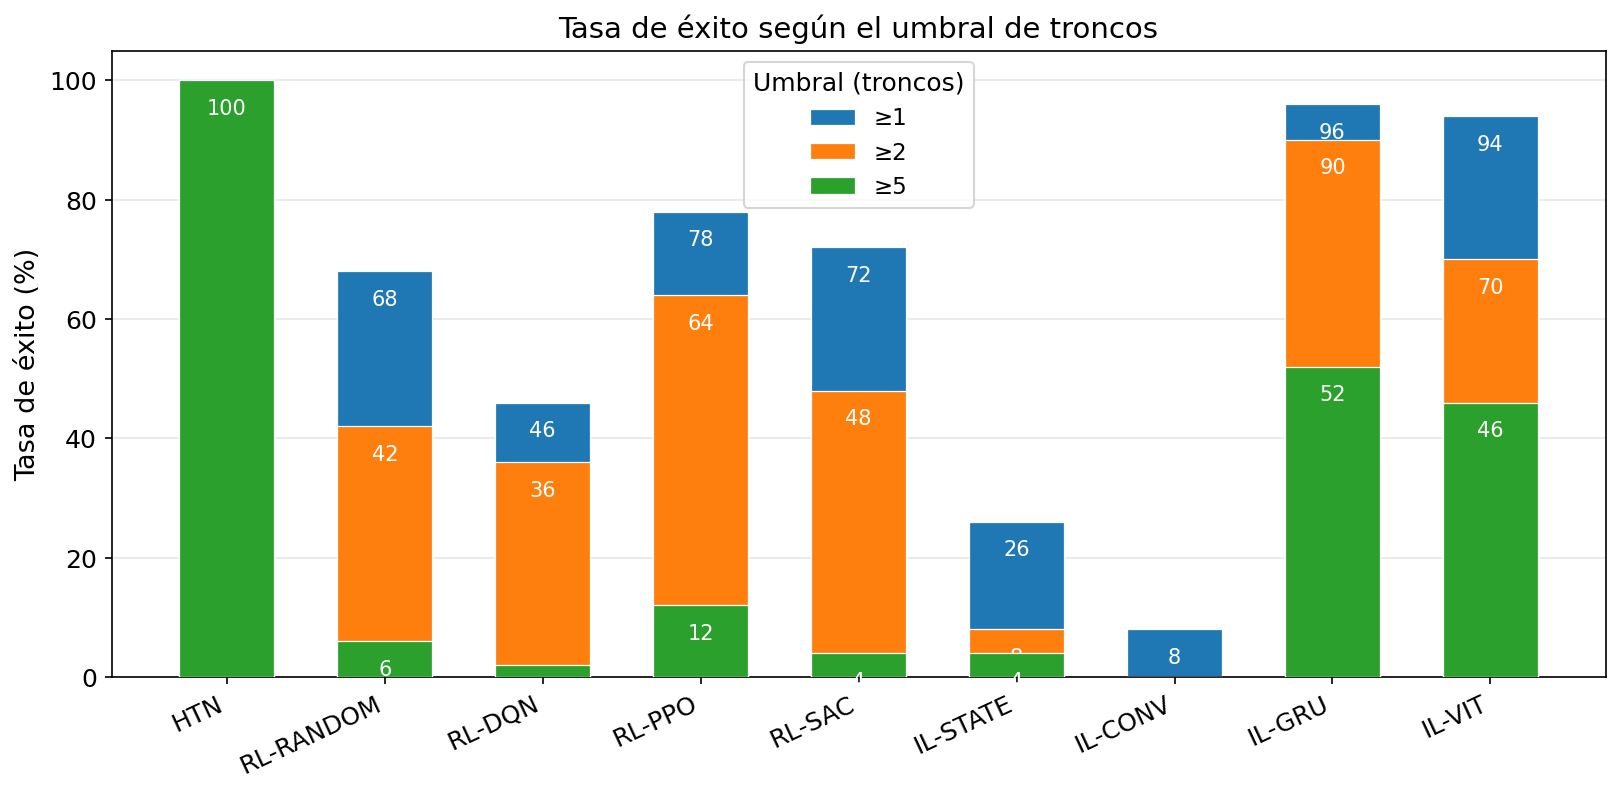
\includegraphics[width=1\textwidth]{imaxes/09_resultados/eval_exito_umbrales_apilado.png}
  }
  \caption[Tasa de éxito según el umbral de troncos]{Tasa de éxito de cada técnica al exigir
  $\geq \num{1}$, $\geq \num{2}$ y $\geq \num{5}$ troncos, superpuestas sobre la misma barra (\num{50} episodios).
  El \gls{htn} mantiene el \qty{100}{\percent} en los tres umbrales; en el resto el éxito decae al subir
  la exigencia, de forma acusada en el refuerzo (PPO: $\num{78}\!\to\!\num{64}\!\to\!\qty{12}{\percent}$) y más contenida
  en IL-GRU ($\num{96}\!\to\!\num{90}\!\to\!\qty{52}{\percent}$).}
  \label{fig:eval-exito-umbrales}
\end{figure}
 \chapter{Conclusiones}
\label{chap:conclusions}

\lettrine{L}{os} objetivos planteados al comienzo del trabajo se han cumplido satisfactoriamente.
El punto de partida fue diseñar una arquitectura común que permitiese a los agentes
compartir entorno, observaciones y protocolo de evaluación, combinando
\textit{Node.js} para el control de bots con \textit{Mineflayer}
y \textit{Python} para los modelos de \gls{ia}.
Además, fue necesario tratar la integración entre el servidor \textit{Java} de \textit{Minecraft},
\textit{Node.js} y \textit{Python}, que fue una fuente constante de problemas de sincronización, aunque la arquitectura final es estable y funcional.
Otra de las dificultades fue la captura de imágenes en tiempo real y tener que almacenarlas junto al
vector de estado al que pertenecían, ya que la obtención de las imágenes y el vector de estado no estaban
sincronizados de base.

Sobre este \gls{framework} se implementaron los tres
agentes: el planificador \gls{htn} (Capítulo~\ref{chap:iter1}), los agentes de imitación
(Capítulo~\ref{chap:iter2}) y los agentes de refuerzo con tres algoritmos distintos
(\gls{dqn}, \gls{ppo} y \gls{sac}) (Capítulo~\ref{chap:iter3}).

Para que el aprendizaje por imitación fuese posible fue necesario crear un conjunto de datos
propio, recogiendo las ejecuciones del planificador \gls{htn} en vivo. 
La comparación entre técnicas exigió definir una evaluación rigurosa y
reproducible (Sección~\ref{sec:eval-metodologia}, página~\pageref{sec:eval-metodologia}):
misma semilla, punto de aparición fijo, número de episodios y una métrica de éxito común
($\geq \num{5}$ troncos talados y recogidos), 
preservando la restricción de no omnisciencia: imagen en primera persona y estado restringido
al \gls{fov}, sin acceso a posiciones exactas ni visión a través de obstáculos.

Los resultados, recogidos en el Capítulo~\ref{chap:discusion-resultados}, permiten extraer
varias conclusiones. La principal es la importancia del conocimiento experto; 
las dos mejores técnicas (\gls{htn} e \gls{il}) son precisamente las que lo utilizan. 
Conviene mencionar que la superioridad del \gls{htn} es intrínseca a este tipo de tareas; al operar sobre conocimiento codificado a mano, siempre va a realizar la tarea de la mejor forma posible. Sin embargo, esa misma dependencia es su límite, ya que su extensión a jerarquías mucho más complejas no es sencilla y exige un esfuerzo de modelado que crece con la complejidad del dominio.
El \gls{il} reduce el coste de entrenamiento respecto al
refuerzo y obtiene un mejor rendimiento, ya que aprende de un experto y puede enfocarse en la
explotación de la tarea en lugar de explorar desde cero. El \gls{rl}, sin embargo, es capaz
de descubrir comportamientos que el experto no enseñó: en la \gls{dqn}, el agente aprende a
talar bloques adyacentes (superior e inferior respecto al bloque talado) 
que el \gls{il} no presenta, y consigue una
navegación más adaptada a su percepción y espacio de acciones. Esta capacidad de
generalización tiene el coste de requerir un presupuesto de cómputo mayor: el espacio
de acciones con temporalidad fija y la recompensa escasa y diferida limitaron el
número de interacciones posibles, evidenciando que la cantidad de recursos es un factor
determinante para esta familia de técnicas. Como se menciona en el
Capítulo~\ref{chap:sota}, la mayoría de trabajos relacionados utilizan presupuestos de
cómputo y datos de magnitudes mucho mayores; bajo un escenario ideal, los agentes
dispondrían de un horizonte de rendimiento significativamente más amplio.

El trabajo utiliza muchas de las competencias enseñadas en la titulación: ingeniería de software,
desde el desarrollo con \textit{Scrum} hasta el uso de \acrshort{http} para la comunicación entre modelos; 
análisis y manejo de datos, con la creación del \textit{dataset} y la
evaluación de los agentes; e inteligencia artificial, desde algoritmos con enfoques clásicos como
\gls{htn} hasta aproximaciones profundas como \gls{rl} e \gls{il}. 
Además, incorpora herramientas fuera del plan de estudios, como
\textit{Node.js}, servidores \textit{Java} o entornos de simulación \textit{3D},
necesarias para llevar el trabajo a cabo, lo que refleja la capacidad de investigar
y adoptar nuevas tecnologías para la realización de proyectos.

\section{Trabajo Futuro}
\label{sec:conclu-futuro}
Las líneas de trabajo más prometedoras aprovechan la complementariedad entre los tres
paradigmas. Por ejemplo, combinar el \gls{htn} como tutor de exploración en un bucle \gls{rl} tipo
\gls{dagger}~\cite{DBLP:journals/jmlr/RossGB11} permitiría guiar al agente de refuerzo con conocimiento
experto y acelerar significativamente su convergencia. En paralelo, ampliar el \textit{dataset} de
demostración y explorar otras arquitecturas para el \gls{il} podría extender sus capacidades.
A más largo plazo, el \gls{framework} desarrollado
ofrece una base para escalar la comparación a tareas de mayor complejidad jerárquica dentro de
\textit{Minecraft}, como la obtención de diamante o la construcción de estructuras.
 %\chapter{Trabajo Futuro}
\label{chap:trabajo_futuro}

\lettrine{L}{a} hipótesis central del trabajo intenta demostrar que las tres familias de técnicas son
complementarias (Capítulo~\ref{chap:conclusions}). Cada familia presenta ventajas frente a las otras; 
la vía más prometedora no es perfeccionar ninguna por separado, sino combinarlas.
Este capítulo recoge aproximaciones futuras que se podrían implementar tras los descubrimientos
de este trabajo.

\paragraph{Inicialización del refuerzo por imitación}
\label{sec:tf-il-rl}
En lugar de entrenar las técnicas de refuerzo desde cero, se puede utilizar la política de imitación
ya entrenada (Capítulo~\ref{chap:iter2}). La red del agente de refuerzo se inicializa 
con los pesos del agente de \gls{il} y el refuerzo 
se encarga únicamente de refinar ese comportamiento y de cubrir lo que la
imitación no aprendió, realizando así un proceso de \gls{fine-tuning}. 

Esta inicialización como arranque del \gls{rl} ataca de frente el problema observado en el
Capítulo~\ref{chap:resultados}: el refuerzo desde cero invierte la mayor parte del cómputo
en aprender lo que la imitación ya tiene aprendido. En el proceso de investigación no se 
encontró literatura que aplicara esta hibridación específica de \gls{rl} con \gls{il} 
en Minecraft.

\paragraph{El planificador como guía de la exploración}
\label{sec:tf-htn-rl}
La segunda hibridación usa el \gls{htn} (Capítulo~\ref{chap:iter1}) como 
\textbf{tutor de exploración} en el entrenamiento. La idea es similar a la de \gls{dagger}, 
pero aplicada al refuerzo: el agente itera sobre el entorno y, 
cuando se desvíe o no sepa qué hacer, el planificador le indica la acción
que él habría tomado, alimentando así su aprendizaje con trayectorias útiles.
Combinada con un algoritmo \emph{off-policy} como \gls{sac}, 
esta guía puede integrarse directamente en el
\gls{replay-buffer}, mezclando transiciones del tutor con las del propio agente.

\paragraph{Ampliación de la cobertura del experto y subredes}
\label{sec:tf-cobertura}
El mayor problema presente en la imitación es la limitación del \gls{dataset}. Al no tener ejemplos de
exploración, el agente no puede aprender a buscar. Como solución se plantea el uso de \textit{subdatasets};
con ellos se podría dividir la tarea en subobjetivos y entrenar subredes especializadas en cada uno de ellos,
las cuales se irían intercambiando entre sí según la situación. Por ejemplo, una subred especializada en \emph{explorar}
se mantendría activa hasta que el agente encontrara un árbol, 
momento en el que se activaría la subred de \emph{aproximación} al árbol, dando paso a la subred de \emph{talado} y, por
último, a la subred de \emph{recogida}.

De esta forma, la recolección del \gls{dataset} se podría paralelizar al poder lanzar varios agentes con tareas más cortas,
abarcando así todas las situaciones posibles que el agente de imitación 
podría encontrarse en la tarea de \gls{woodcutting}.

\paragraph{Escalado de la tarea}
\label{sec:tf-escalado}
Todas las técnicas se evaluaron sobre la tarea de \gls{woodcutting}, una de las tareas
más simples de la jerarquía de progresión de Minecraft (Capítulo~\ref{chap:introduccion}). El siguiente
paso es ascender por esa jerarquía (fabricar una mesa de trabajo, un pico de
madera, recolectar piedra) hasta tareas de horizonte mucho más largo,
como la obtención del pico de hierro o de diamantes. 

\paragraph{Introducción de otras técnicas de aprendizaje}
\label{sec:tf-otras-tecnicas}
Si bien las familias de técnicas estudiadas abarcan un amplio espectro de enfoques, 
existen otras técnicas que también presentan un fuerte potencial. Como se menciona en el Capítulo~\ref{chap:sota}, el proyecto
MindCraft~\cite{mindcraft2025} intenta completar todo el juego (una tarea con un horizonte extremadamente
largo) utilizando únicamente modelos de lenguaje \gls{llm}, sin ningún tipo de intervención humana más
allá de la inicialización. Además, incluye varias aproximaciones como \gls{mas}, en la que múltiples agentes
trabajan en conjunto para resolver la tarea.

Dada la capacidad de los \gls{llm} para generar código y sus altas ventanas de contexto, la posibilidad
de completar buena parte de la jerarquía de progresión de Minecraft con estas técnicas es 
un área de investigación muy prometedora.

 %%%%%%%%%%%%%%%%%%%%%%%%%%%%%%%%%%%%%%%%
 % Apéndices, glosarios e bibliografía  %
 %%%%%%%%%%%%%%%%%%%%%%%%%%%%%%%%%%%%%%%%

\appendix
\appendixpage
\chapter{Jerarquía de un Pico de Hierro}
\label{apx:iron-pickaxe}

\begin{figure}[htbp]
    \centering
    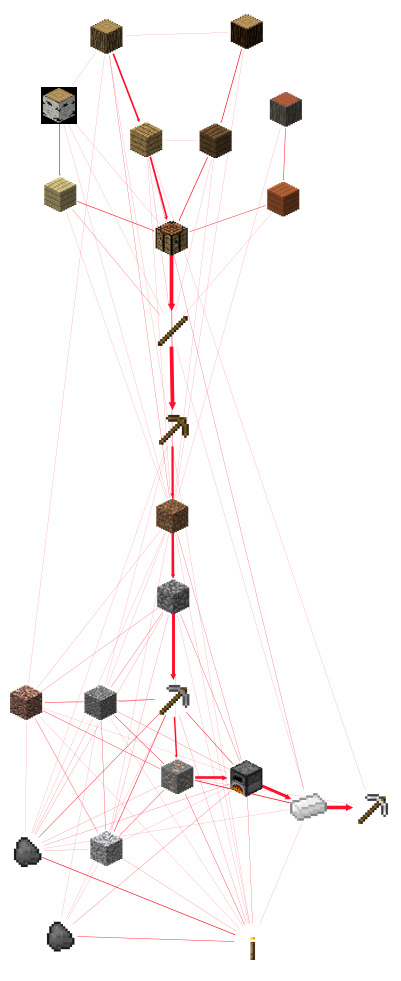
\includegraphics[width=0.3\linewidth]{imaxes/anexos/iron_graph.png}
    \caption[Jerarquía de dependencias para obtener un pico de hierro en \textit{Minecraft}.]
    {Jerarquía de dependencias para obtener un pico de hierro en \textit{Minecraft}. Se pueden observar las dependencias necesarias:
    \textit{Pico de Madera} $\rightarrow$ \textit{Pico de Piedra} $\rightarrow$ \textit{Pico de Hierro}. Adaptada de 
    \textit{MineRL}~\cite{guss2019minerl}.}
    \label{fig:iron-pickaxe}
\end{figure}
\chapter{Frame del dataset de demostraciones}
\label{apx:frame}

\lettrine{E}{n} este apéndice se muestra un ejemplo real de un \emph{frame} del
conjunto de demostraciones generado por el agente simbólico
(Capítulo~\ref{chap:iter1}). Cada \emph{frame} es un par \textit{OBSERVACIÓN-ACCIÓN}: la
imagen del visor en primera persona (Figura~\ref{fig:apx-frame}, página~\pageref{apx:frame}) junto con el
registro JSON de su estado, su acción y los metadatos de percepción
(Listado~\ref{lst:frame}, página~\pageref{lst:frame}).

\begin{figure}[hp!]
  \centering
  \resizebox{\textwidth}{!}{
  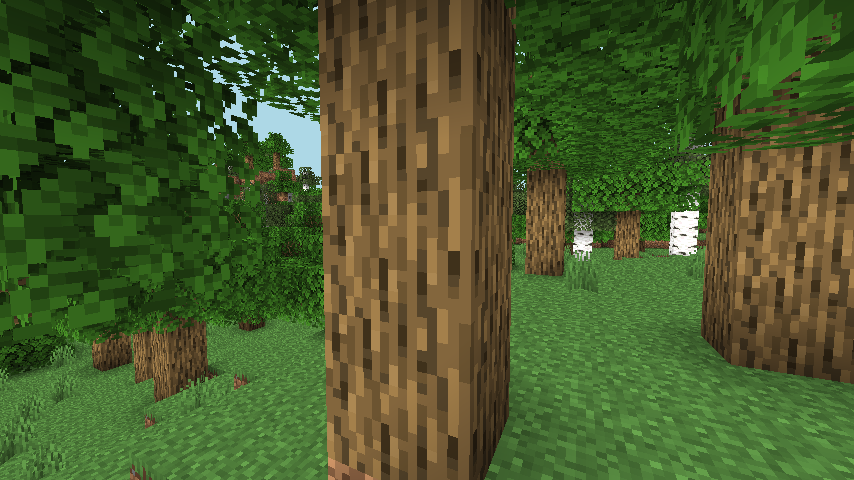
\includegraphics[width=0.8\textwidth]{imaxes/anexos/imagen_visor.png}
  }
  \caption[Imagen del visor en primera persona]{Imagen del visor en primera persona asociada al \emph{frame} del
  Listado~\ref{lst:frame} (página~\pageref{lst:frame}): el agente apunta a un tronco situado a $2{,}7$ bloques y
  ejecuta la acción \texttt{attack}.}
  \label{fig:apx-frame}
\end{figure}

\clearpage
\begin{lstlisting}[caption={Registro JSON de un \emph{frame} (par \textit{OBSERVACIÓN-ACCIÓN}) del dataset de demostraciones.},label={lst:frame}]
{
  "image": "data/recordings/Rec_100_ablgs0_screenshots/frame_00003.png",
  "state": {
    "x": 11.499,
    "y": 123,
    "z": 6.581,
    "yaw": -3.1416,
    "pitch": -0.343
  },
  "action": "attack",
  "camera_delta": {
    "dyaw": 0,
    "dpitch": 0
  },
  "session_id": "Rec_100_ablgs0",
  "tree_visible": true,
  "tree_distance": 2.7
}
\end{lstlisting}

En este \emph{frame}, el agente tiene un tronco visible a $2{,}7$ bloques
(\texttt{tree\_visible}~=~true) y ejecuta la acción \texttt{attack} sin
desplazamiento de cámara (\texttt{camera\_delta} nulo), correspondiente al instante
en que tala el árbol que tiene enfrente. 
\chapter{Árbol de Tareas para la Obtención de un Pico de Hierro}
\label{apx:htn-iron-decomp}
\lettrine{E}{n} este apéndice se muestra la descomposición completa de tareas \gls{htn} 
para la obtención de un pico de hierro en \textit{Minecraft}, mostrando la jerarquía de tareas
y subtareas que componen cada fase de la progresión (madera, piedra e hierro). Así como las
tareas de recuperación. 

\begin{figure}[hp!]
  \centering
  \begin{forest}
    for tree={
      font=\footnotesize, grow'=0, folder, rounded corners, draw,
      edge={-, semithick}, l sep=4mm, s sep=1.2mm, anchor=west,
      inner sep=2.5pt,
    },
    compuesta/.style={fill=blue!8},
    [{Obtener pico de hierro}, compuesta
      [{Fase madera (Ver Figura \ref{fig:htn-wood})}, compuesta]
      [{Fase piedra (Ver Figura \ref{fig:htn-stone})}, compuesta]
      [{Fase hierro (Ver Figura \ref{fig:htn-iron})}, compuesta]
    ]
  \end{forest}
  \caption[Árbol de descomposición general del agente simbólico]{Árbol de descomposición general de la progresión
  hasta el pico de hierro. Las subtareas detalladas de cada fase se desglosan en figuras posteriores.}
  \label{fig:htn-general}
\end{figure}

\begin{figure}[hp!]
  \centering
  \begin{forest}
    for tree={
      font=\footnotesize, grow'=0, folder, rounded corners, draw,
      edge={-, semithick}, l sep=4mm, s sep=1.2mm, anchor=west,
      inner sep=2.5pt,
    },
    compuesta/.style={fill=blue!8},
    primitiva/.style={fill=green!12},
    recup/.style={fill=red!10},
    [{Fase madera}, compuesta
      [{Recolectar madera \textit{(chop $\times$5)}}, primitiva]
      [{Fabricar tablones \textit{(craftItem)}}, primitiva]
      [{Colocar mesa de trabajo \textit{(ensureCraftingTable)}}, compuesta
        [{Recolectar madera (si no está en el inventario) \textit{(chop $\times$5)}}, recup]
        [{Fabricar tablones \textit{(craftItem)}}, primitiva]
        [{Colocar mesa de trabajo \textit{(placeBlock)}}, primitiva]
      ]
      [{Fabricar pico de madera \textit{(craftItem)}}, primitiva]
    ]
  \end{forest}
  \caption[Tarea HTN: Fase Madera]{Detalle del árbol de descomposición para la Fase madera. 
  Esta fase inicia la progresión y reutiliza primitivas y tareas de recuperación como el \gls{woodcutting}.}
  \label{fig:htn-wood}
\end{figure}

\begin{figure}[hp!]
  \centering
  \begin{forest}
    for tree={
      font=\footnotesize, grow'=0, folder, rounded corners, draw,
      edge={-, semithick}, l sep=4mm, s sep=1.2mm, anchor=west,
      inner sep=2.5pt,
    },
    compuesta/.style={fill=blue!8},
    primitiva/.style={fill=green!12},
    [{Fase piedra}, compuesta
      [{Minar piedra \textit{(ensureEquipped + mineBlock)}}, compuesta
        [{Comprobar la herramienta equipada}, primitiva]
        [{Si no hay pico de madera, fabricar uno}, compuesta
          [{Fase madera \textit{(Ver Figura \ref{fig:htn-wood})}}, compuesta]
        ]
        [{Minar piedra $\times$14}, primitiva]
      ]
      [{Fabricar 2 picos de piedra \textit{(craftItem)}}, primitiva]
    ]
  \end{forest}
  \caption[Tarea HTN: Fase Piedra]{Detalle del árbol de descomposición para la Fase piedra. 
  Si no se dispone de la herramienta adecuada, se invoca la Fase madera para su creación.}
  \label{fig:htn-stone}
\end{figure}

\begin{figure}[hp!]
  \centering
  \begin{forest}
    for tree={
      font=\footnotesize, grow'=0, folder, rounded corners, draw,
      edge={-, semithick}, l sep=4mm, s sep=1.2mm, anchor=west,
      inner sep=2.5pt,
    },
    compuesta/.style={fill=blue!8},
    primitiva/.style={fill=green!12},
    [{Fase hierro}, compuesta
      [{Buscar mineral de hierro \textit{(heurística)}}, compuesta
        [{Comprobar si hay hierro visible}, primitiva]
        [{Si no hay, explorar hasta encontrarlo}, compuesta]
      ]
      [{Minar mineral de hierro \textit{(ensureEquipped + mineBlock)}}, compuesta
        [{Comprobar la herramienta equipada}, primitiva]
        [{Si no hay pico de piedra, fabricar uno}, compuesta
          [{Fase piedra \textit{(Ver Figura \ref{fig:htn-stone})}}, compuesta]
        ]
        [{Minar hierro $\times$3}, primitiva]
      ]
      [{Buscar carbón \textit{(heurística)}}, compuesta
        [{Comprobar si hay carbón visible}, primitiva]
        [{Si no hay, explorar hasta encontrarlo}, compuesta]
      ]
      [{Minar carbón \textit{(ensureEquipped + mineBlock)}}, compuesta
        [{Comprobar la herramienta equipada}, primitiva]
          [{Si no hay pico de piedra, fabricar uno}, compuesta
            [{Fase piedra \textit{(Ver Figura \ref{fig:htn-stone})}}, compuesta]
          ]
          [{Minar carbón $\times$3}, primitiva]
      ]
      [{Fundir hierro \textit{(horno + smeltItem)}}, compuesta
        [{Fabricar horno \textit{(craftItem)}}, primitiva]
        [{Colocar horno \textit{(placeBlock)}}, primitiva]
        [{Fundir hierro \textit{(smeltItem)}}, primitiva]
      ]
      [{Fabricar pico de hierro \textit{(craftItem)}}, primitiva]
    ]
  \end{forest}
  \caption[Tarea HTN: Fase Hierro]{Detalle del árbol de descomposición para la Fase hierro, 
  incluyendo la búsqueda heurística de minerales y el proceso de fundición.}
  \label{fig:htn-iron}
\end{figure}
\chapter{Variantes de imitación}
\label{apx:il-curvas}

\lettrine{E}{ste} apéndice recoge las curvas de entrenamiento de las cuatro
variantes comparadas en la Iteración~II
(Capítulo~\ref{chap:iter2}) en la Tabla~\ref{tab:progresion-il} (página~\pageref{tab:progresion-il}),
todas bajo la misma configuración (igual partición e hiperparámetros, variando solo el
extractor). Se muestran juntas para ilustrar el sobreajuste que exhiben los modelos
dado el tamaño limitado del dataset de demostraciones y la similitud entre sus clases,
siendo la variante \gls{vit} el caso más pronunciado.

\begin{figure}[htbp]
  \vfill
  \centering
  \begin{minipage}{0.45\textwidth}
    \centering
    \textbf{\small Solo estado}\\[2mm]
    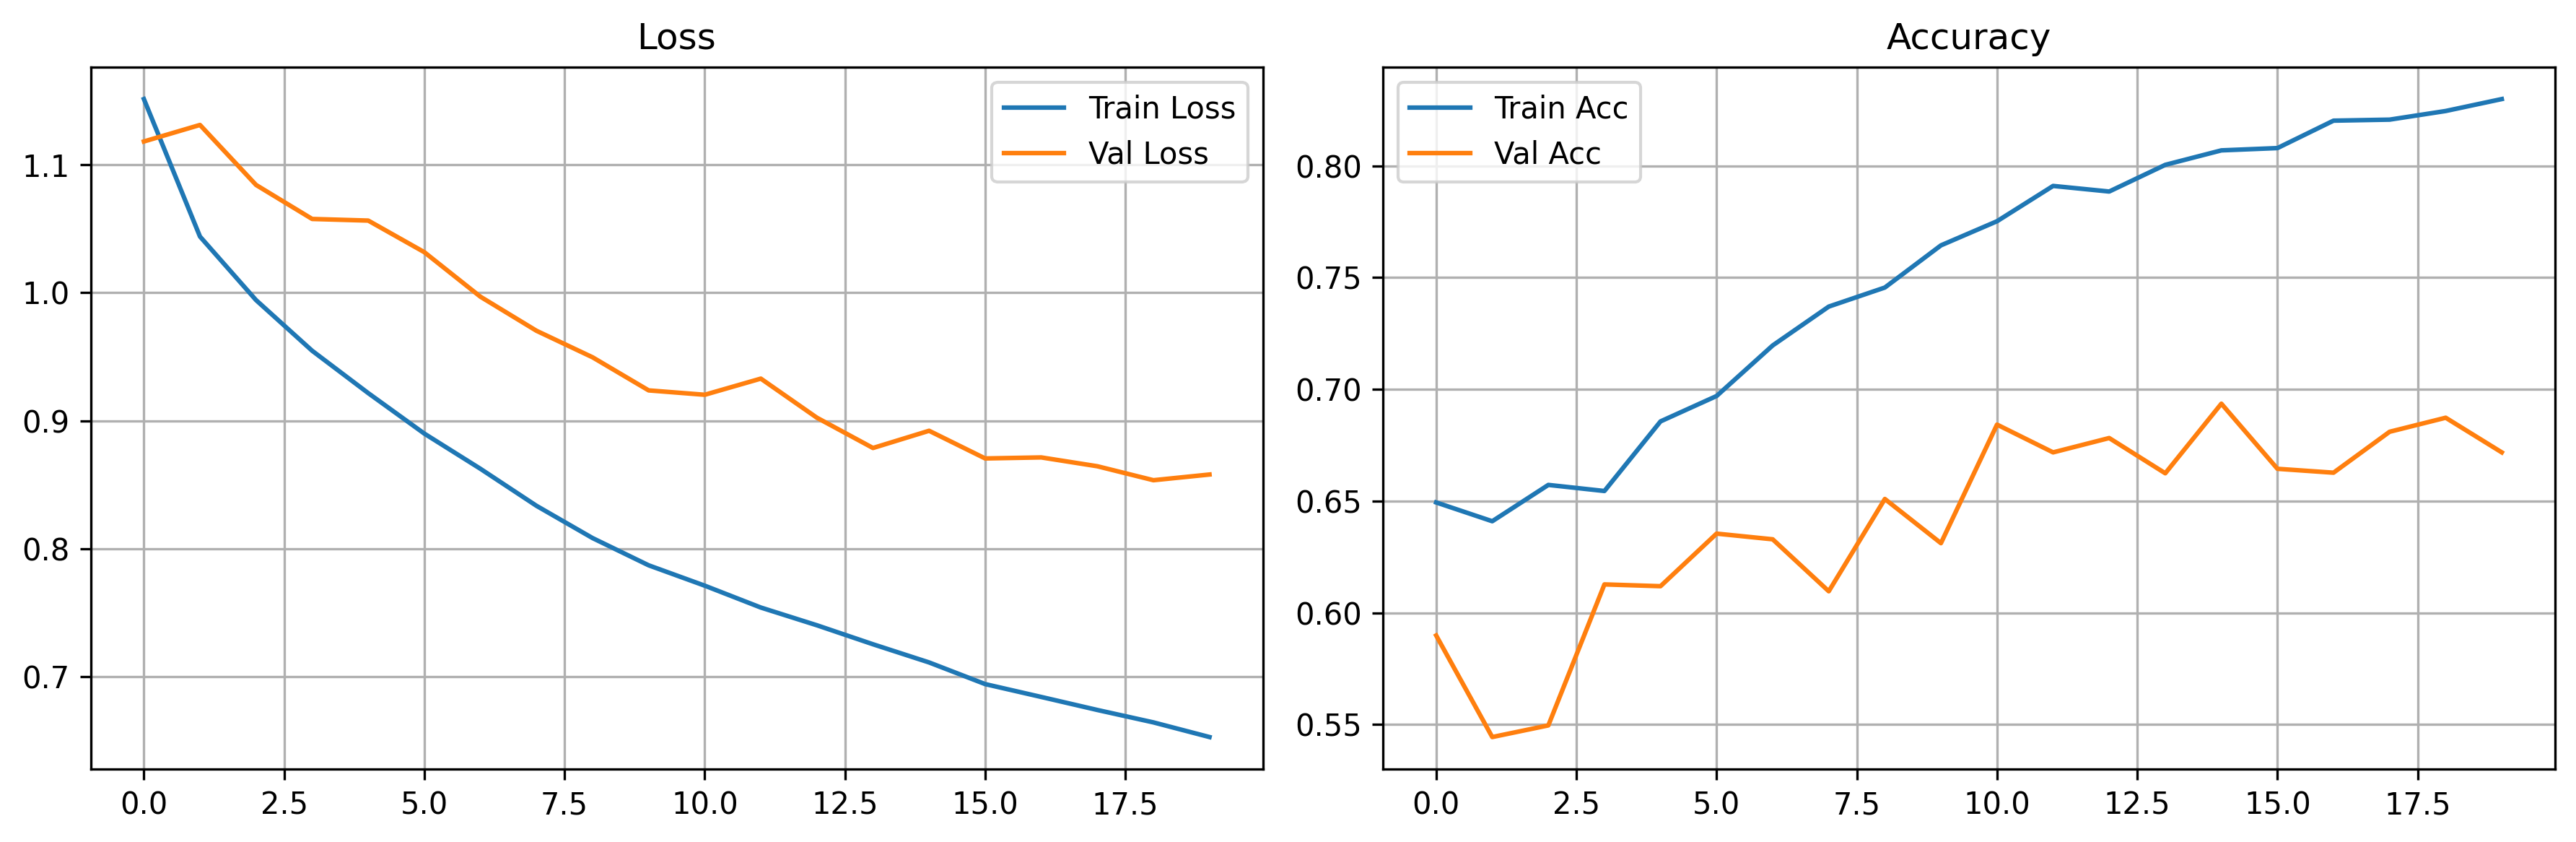
\includegraphics[width=\linewidth]{imaxes/anexos/il_curve_state.png}
  \end{minipage}\hfill
  \begin{minipage}{0.45\textwidth}
    \centering
    \textbf{\small Visual (\gls{gru})}\\[2mm]
    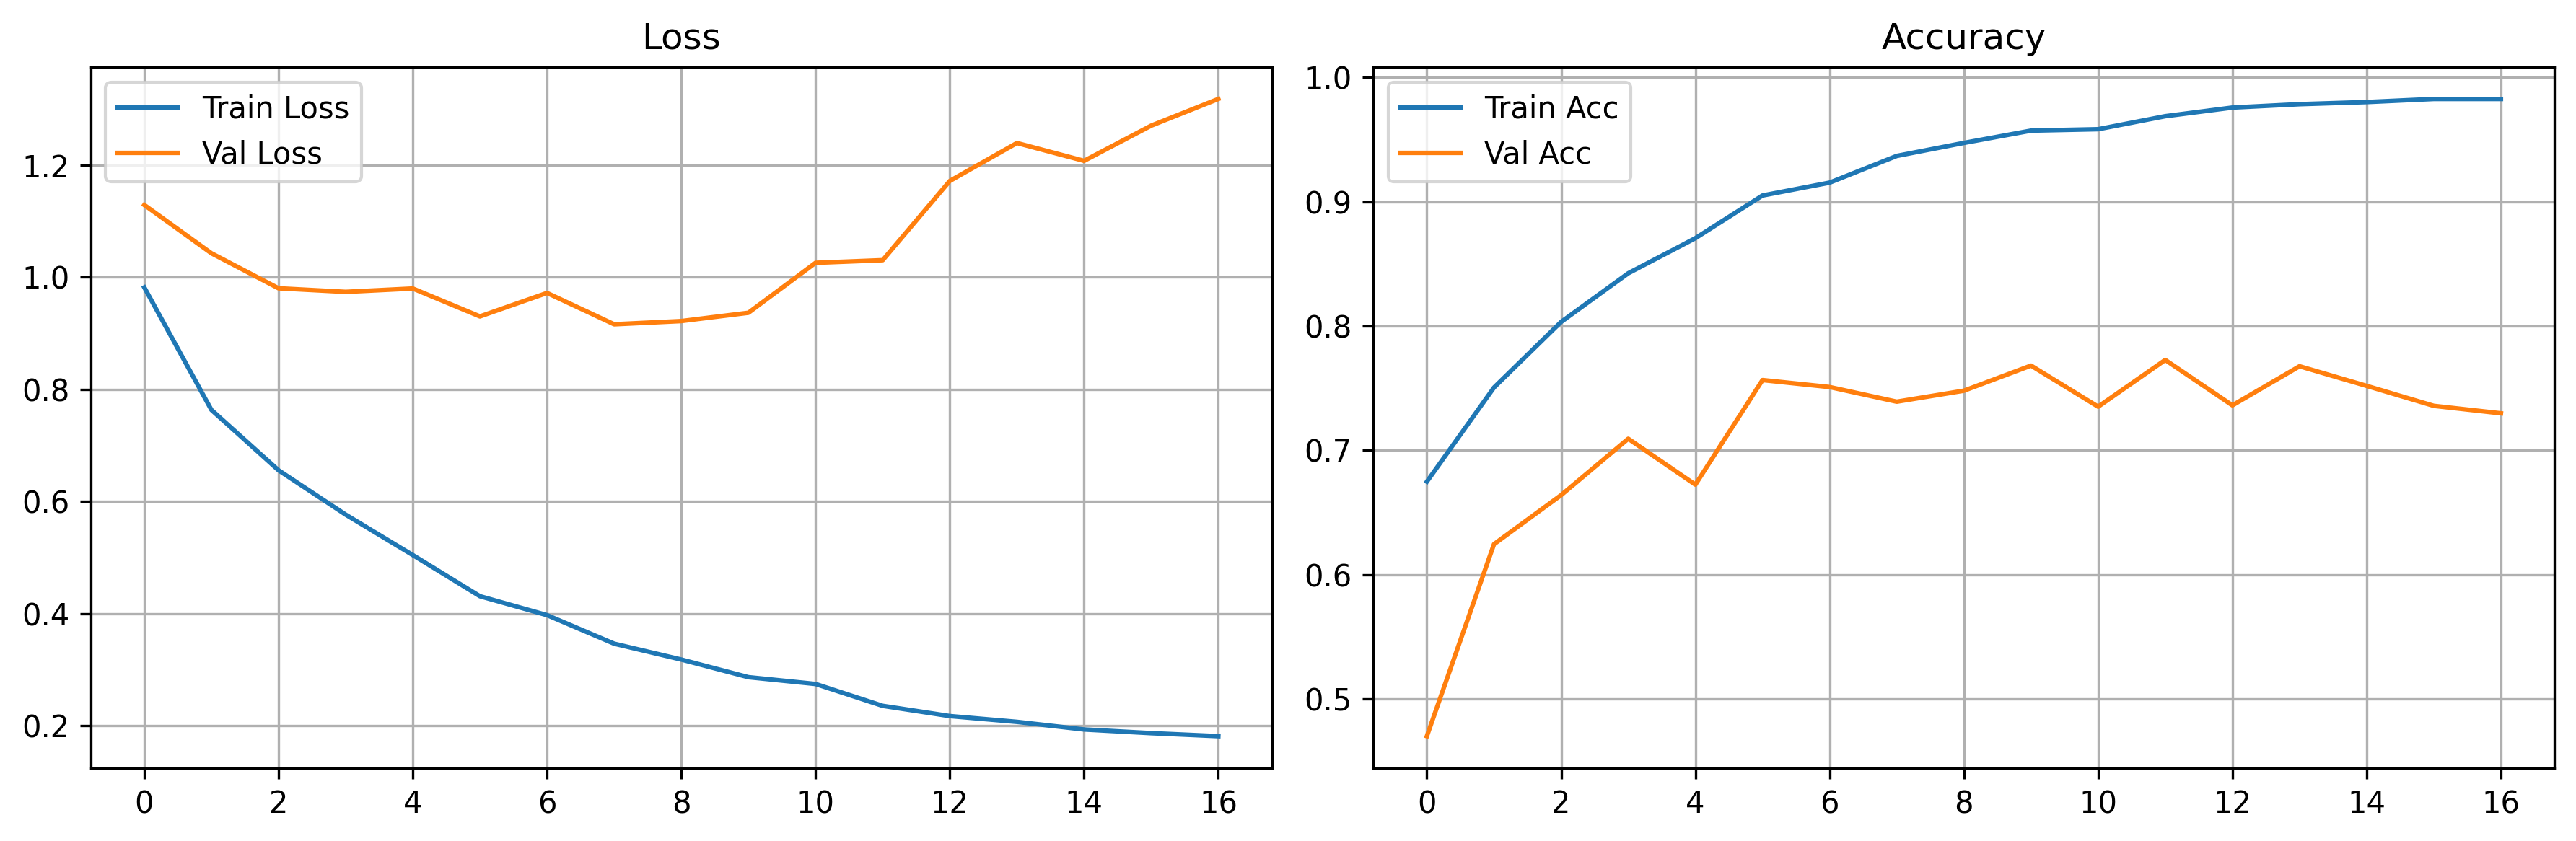
\includegraphics[width=\linewidth]{imaxes/anexos/il_curve_gru.png}
  \end{minipage}

  \vfill

  \begin{minipage}{0.45\textwidth}
    \centering
    \textbf{\small Visual (\gls{convlstm})}\\[2mm]
    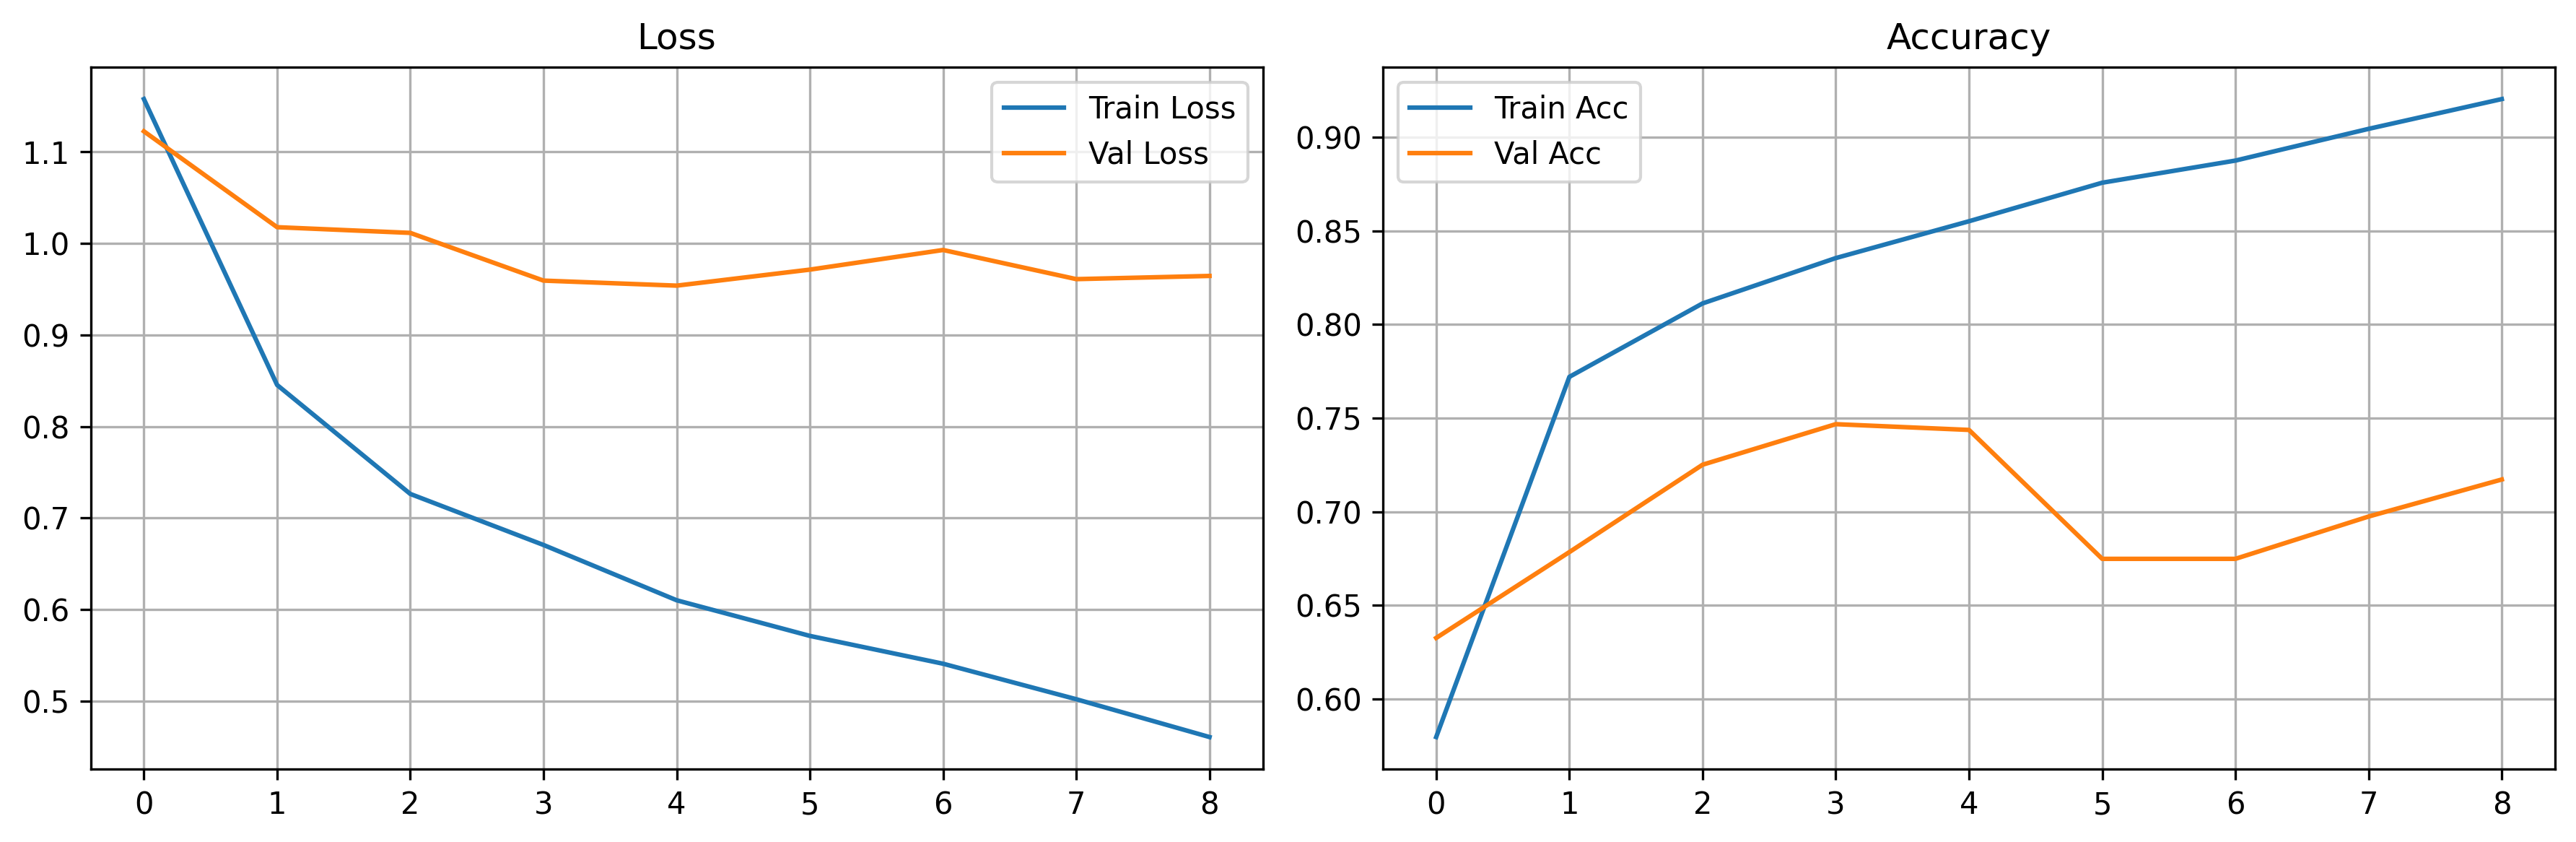
\includegraphics[width=\linewidth]{imaxes/anexos/il_curve_convlstm.png}
  \end{minipage}\hfill
  \begin{minipage}{0.45\textwidth}
    \centering
    \textbf{\small Visual (\gls{vit})}\\[2mm]
    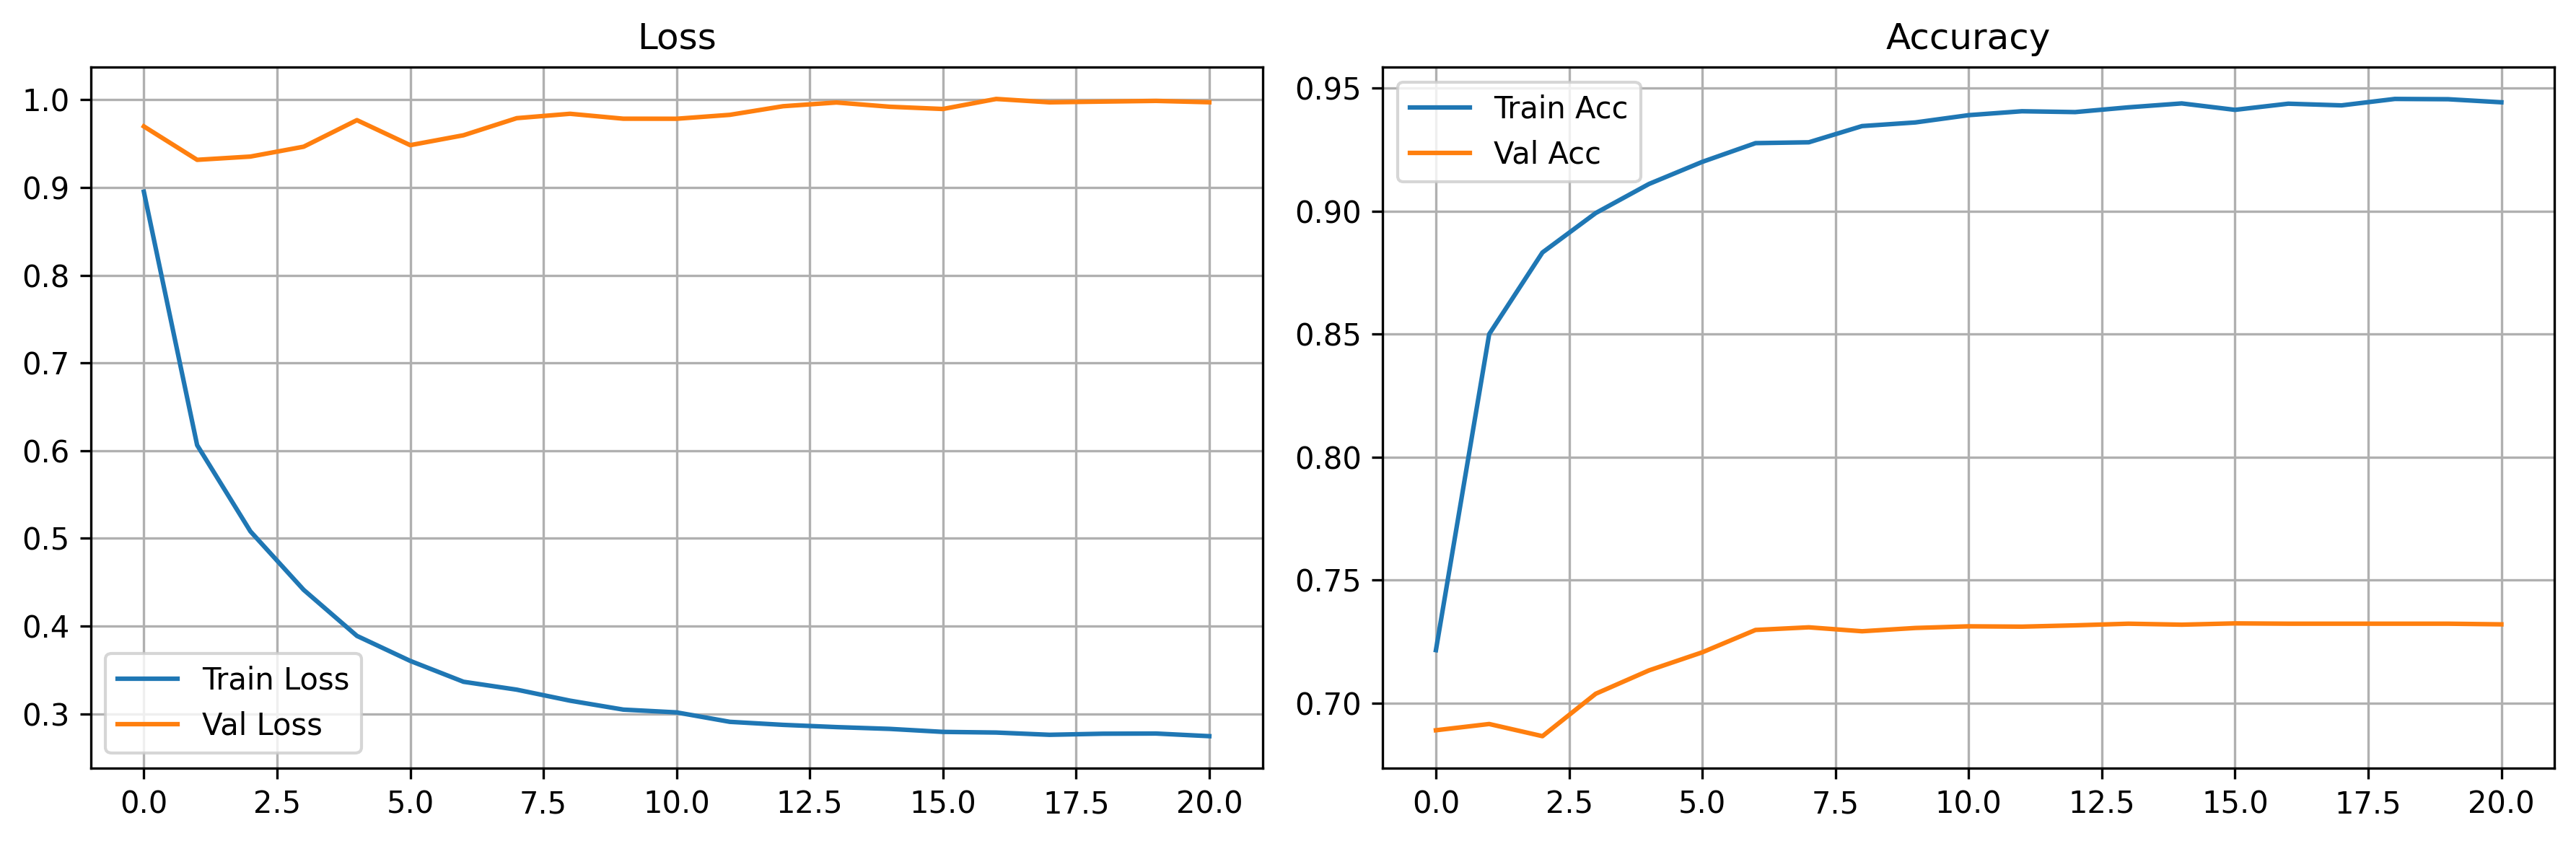
\includegraphics[width=\linewidth]{imaxes/anexos/il_curve_vit.png}
  \end{minipage}
  \vfill

  \caption[Curvas de entrenamiento de las variantes de imitación]{Curvas de
  entrenamiento (precisión y pérdida en entrenamiento y validación) de las cuatro
  variantes bajo configuración idéntica. El modelo de solo estado no alcanza
  una precisión de validación satisfactoria (cota inferior). Las variantes \gls{gru}
  y \gls{convlstm} generalizan de forma razonable, con una brecha
  entre entrenamiento y validación contenida. La variante \gls{vit} presenta el sobreajuste
  más pronunciado: su precisión de entrenamiento alcanza el ${\sim}$\num{95}\% mientras la
  de validación se estanca en torno al \num{72}--\num{73}\%, una brecha de más de \num{20}\%
  que evidencia que su mayor capacidad no se traduce en mejor generalización con un
  dataset de este tamaño.}
  \label{fig:apx-il-curvas}
\end{figure}

\glsaddall

\printglossary[type=\acronymtype,title=\nomeglosarioacronimos]
\printglossary[title=\nomeglosariotermos]

\bibliographystyle{IEEEtranN}
\bibliography{\bibconfig,bibliografia/bibliografia}
\clearpage
 
\end{document}

%%%%%%%%%%%%%%%%%%%%%%%%%%%%%%%%%%%%%%%%%%%%%%%%%%%%%%%%%%%%%%%%%%%%%%%%%%%%%%%%